% Organizing document for the ssu-align User's Guide
%
% SVN $Id: main.tex 2375 2008-03-31 22:24:06Z nawrockie $

\documentclass[10pt]{article}
\usepackage[pdftex]{graphicx}  
\usepackage{html}		% From the LaTeX2html translator
\usepackage{apalike}
\usepackage{rotating}
\usepackage{fullpage}
\usepackage{times}
\usepackage{fancyvrb}
\usepackage{verbatim}
\usepackage{rotating}

\setcounter{secnumdepth}{1}

\renewcommand{\familydefault}{\sfdefault}
% customizations used in the User's Guide


% Description-like environment for documenting functions/APIs.
% puts the description label in a minipage with a large hanging
% indent.
% Good christ this took a long time to develop.
% hanging indent trick stolen from Peter Wilson's hanging.sty @CTAN
% minipage allows multi-line label, and puts item on next line.
% customized list inspired by Kopka/Daly _Guide to LaTeX_ p.213
% SRE, Wed Dec 27 11:37:18 2000
%
\newenvironment{sreapi}{%
     \begin{list}{}{%
       \renewcommand{\makelabel}[1]{%
         \begin{minipage}{\textwidth}%
           \hangindent10em\hangafter1\noindent%
           {\bfseries\texttt{##1}\vspace{0.8em}}%
         \end{minipage}%
     }}}%
     {\end{list}}

% Description-like environment for producing lists like:
%
%     label  stuff, stuff, stuff
%
%    label2  more stuff, more stuff,
%            more stuff.
% \begin{sreitems}{Longest label} \item[label] stuff, ... \end{sreitems}
% SRE, Wed Dec 27 11:59:43 2000
%
\newenvironment{sreitems}[1]{%
     \begin{list}{}{%
       \settowidth{\labelwidth}{#1}%
       \setlength{\leftmargin}{\labelwidth}%
       \addtolength{\leftmargin}{\labelsep}%
       }}
     {\end{list}}
       
\DefineVerbatimEnvironment{sreoutput}{Verbatim}{fontsize=\scriptsize,xleftmargin=2.0\parindent}%
\DefineVerbatimEnvironment{sreoutputtiny}{Verbatim}{fontsize=\tiny,xleftmargin=2.0\parindent}%
\DefineVerbatimEnvironment{sreoutputtinywide}{Verbatim}{fontsize=\tiny,xleftmargin=0.0\parindent}%

\makeatletter
\newcommand{\listoffaqs}{\@starttoc{faq}}
\newenvironment{srefaq}[1]
{\addcontentsline{faq}{faq}{#1}\begin{sloppypar}\noindent\slshape\small\begin{quote}\textbf{$\triangleright$ #1}}
{\end{quote}\end{sloppypar}}
\newcommand{\l@faq}[2]{\@dottedtocline{0}{0pt}{0pt}{#1}{#2}}
\makeatother


% Consistent font styles
%   \software{} for the name of a software package
%   \database{} for the name of a database
%   \prog{}     for a program or file name
%   \emprog{}   for an emphasized program or file name
%   \user{}     for a typed user command

\newcommand{\sft}[1]{\textsc{#1}}
\newcommand{\db}[1]{\textsc{#1}}
\newcommand{\software}[1]{\textsc{#1}}
\newcommand{\database}[1]{\textsc{#1}}
\newcommand{\prog}[1]{{\small\bfseries\texttt{#1}}}
\newcommand{\emprog}[1]{{\small\bfseries\texttt{#1}}}
\newcommand{\user}[1]{\indent\indent{\small\bfseries\texttt{> #1}}}
\newcommand{\scriptuser}[1]{\indent\indent{\scriptsize\bfseries\texttt{> #1}}}

% The ``wideitem'' environment is mostly obsolete, but
% it gets used in converted manpages.
\newenvironment{wideitem}{\begin{list} 
     {}
     { \setlength{\labelwidth}{2in}\setlength{\leftmargin}{1.5in}}}
     {\end{list}}


% The following are used as temp vars in how man pages are 
% converted into LaTeX w/ rman; see ``make manpages'' in Makefile.
\newlength{\sresavei}
\newlength{\sresaves}



\begin{document}

\bibliographystyle{apalike}

\begin{titlepage}
{\Large

\vspace*{\fill}

%\begin{latexonly}
%\noindent
%%{\Huge \texttt{ssu-align} \textsf{ User's Guide}} \\ 
%{\Huge SSUalign User's Guide} \\ 
%\rule[2pt]{\textwidth}{1pt} \\
%\hspace*{\fill} {\large \textsf{Structural alignment of small subunit
%    ribosomal RNA sequences}\\}
%\end{latexonly}

%\begin{htmlonly}
\begin{center}
{\Huge \textbf{\textsc{ssu-align} \huge{User's Guide}}}\\
{\large \textbf{Structural alignment of small subunit ribosomal RNA
    sequences}}\\
\end{center}
%\end{htmlonly}

\vspace*{\fill}

\begin{center}
\textsl{\htmladdnormallink{http://infernal.janelia.org/}{http://infernal.janelia.org/}}\\
Version @RELEASE@; @RELEASEDATE@ \\ 

\vspace*{\fill}

Eric Nawrocki and Sean Eddy\\
HHMI Janelia Farm\\
19700 Helix Drive\\
Ashburn VA 20147\\
\textsl{\htmladdnormallink{http://selab.janelia.org/}{http://selab.janelia.org}} \\
\end{center}

\vspace*{\fill}

}
\end{titlepage}

\vspace*{\fill}
\begin{flushleft}
Copyright (C) 2009 HHMI Janelia Farm Research Campus.

\vspace{2em} 

\software{ssu-align} and \software{infernal}'s source code and documentation are freely
redistributable and modifiable under the terms of the GNU General
Public License (GPL), version 3.
\end{flushleft}

\newpage
\tableofcontents

\newpage
\section{Introduction}

SSU-ALIGN identifies and aligns small subunit ribosomal RNA
(SSU rRNA) genes in sequence datasets. It uses models of the primary
sequence and secondary structure conservation of SSU rRNA as inferred
by comparative sequence analysis and confirmed by crystal structure
determination from the \db{comparative rna website} (\db{crw}) 
(\htmladdnormallink{http://www.rna.ccbb.utexas.edu/}{http://www.rna.ccbb.utexas.edu/})
\cite{CannoneGutell02}.

\subsection{Overview}
The SSU-ALIGN package contains six different
programs: \prog{ssu-align}\footnote{SSU-ALIGN is the name of the
  software package as well as the name of one of the programs within
  the package. In this guide, when written in lowercase bold-faced
  type (\prog{ssu-align}) it refers to the executable program, and
  when written in all capital letters (SSU-ALIGN) it refers to
  the package.},
\prog{ssu-build}, \prog{ssu-draw}, 
\prog{ssu-mask}, \prog{ssu-merge}, and \prog{ssu-prep}. 

Suppose you have a dataset of SSU rRNA sequences from a PCR-based
environmental survey. You can use \prog{ssu-align} to create
structure-based multiple sequence alignments of the
SSU sequences using profile probabilistic models call covariance
models (CMs). \prog{ssu-align} will determine whether each sequence
is archaeal, bacterial or eukaryotic and output a multiple alignment
for each domain that was assigned at least one sequence. 
The \prog{ssu-mask} program can then be used to identify and remove
columns that are not reliably aligned. This step is important prior to using the
alignments as input to phylogenetic inference tools that rely heavily
on alignment accuracy.  
%Alignment columns are selected for removal
%based on automatically calculated ``confidence estimates'' for the
%aligned residues, which are the probabilities that each residue
%belongs in each column of the alignment given the CM. This is
%discussed in more detail in the section 3 of this guide.
The \prog{ssu-draw} program can be used to create secondary
structure diagrams of your alignments. Diagrams that display per-column
alignment statistics, such as information content and frequency of
insertions and deletions, as well as those that display individual
aligned sequences can be drawn.

The \prog{ssu-prep} and \prog{ssu-merge} programs allow users to
divide up large alignment jobs into sets of parallel
\prog{ssu-align} jobs on clusters or multi-core computers.

\prog{ssu-build} can be used to create different models than the
default archaeal, bacterial, and eukaryotic ones. For example, you
might want to build a model that represents a more specific
phylogenetic range, like the \emph{Firmicutes} bacterial phyla to
create maximally precise \emph{Firmicutes} SSU alignments. Or you can build
truncated versions of the default models that model only a
specific region of SSU, such as the V4 hypervariable region.

\subsection{ssu-align's search and alignment stages}

Given an input dataset of unaligned SSU sequences, \prog{ssu-align}
proceeds through two stages to generate alignments as depicted in
figure~\ref{fig:strategy}.  
%In stage 1, each of the sequences is aligned to each of
%the three models based on primary sequence conservation to obtain a
%score for each sequence to each model.  The model that gives the
%highest scoring alignment to each sequence is the \emph{best-matching
%  model} for that sequence.  In stage 2, each sequence is aligned to
%its best-matching model using both primary sequence and secondary
%structure conservation information. The end result is a separate
%multiple alignment for each model that was the best-matching model for
%at least one sequence in the input dataset.
In the first stage, each target sequence is scored with each of the
models based only on sequence conservation. This is done with a
profile HMM derived from each CM, which is significantly faster than
using the CM\@.  The model whose profile HMM gives the highest score to
each sequence is defined as the \emph{best-matching} model for that
sequence. If this highest score is not above a predefined threshold,
the sequence is discarded and not evaluated further. The boundaries of
the best-matching HMM alignment are used to truncate each target
sequence if the alignment does not span the entire target length.  In
stage 2, each surviving, and possibly truncated, sequence is aligned
to its best-matching model, this time using the CM which scores
both sequence and conserved structure. Up to $N$ alignments are
created, one for each model that was the best-match to at least one
target sequence.

\subsection{What distinguishes SSU-ALIGN from other SSU
  alignment tools}

%SSU-ALIGN is a freely available, open source software program
%for creating large-scale alignments of small subunit ribosomal RNA
%(SSU) using covariance models (CMs). The archaeal, bacterial,
%chloroplast, 
%and eukaryotic (nuclear) 
%and mitochondrial 
%SSU CMs in SSU-ALIGN are built from structural seed alignments derived from
%Robin Gutell's Comparative RNA Website (CRW) \cite{CannoneGutell02}.
%Though only a prototype which I hope to develop and extend in the
%future, 
%The following features distinguish SSU-ALIGN from other
%SSU alignment programs (reviewed in chapter 7 of \cite{Nawrocki09b}):

\begin{itemize}

\item \textbf{Structural alignments are calculated at roughly one
  second per sequence.}  

  CM alignment explicitly takes into account conserved sequence and
  well-nested structure. In the past, the slow speed of CM alignment
  has prevented their application to SSU alignment, but recent sequence-based
  acceleration heuristics \cite{Brown00,Nawrocki09b} have 
  made large-scale SSU CM alignment feasible.

\item \textbf{Alignment-specific masks for removing ambiguously aligned columns are
  automatically generated.}
  
  CMs are probabilistic models that allow calculation of the posterior
  probability that each sequence nucleotide belongs in each column of
  the output alignment given the model. Regions of low posterior
  probabilities are indicative of high alignment ambiguity and should
  be pruned away (masked out) prior to phylogenetic
  inference. \prog{ssu-mask} automatically detects and remove these
  columns for any alignment it generates. This is discussed in more
  detail in the section ~\ref{sec:background} of this guide.

\item \textbf{Accurate alignments can be computed using seed
  alignments of less than one hundred sequences.}

  CMs built from small seed alignments of dozens of sequences
  can achieve comparable accuracy to nearest-neighbor based alignment
  methods that use seed (reference) alignments of thousands or tens of
  thousands of sequences. This reduces the level of manual curation
  necessary for creating useful seeds, making it easier to extend
  SSU-ALIGN by adding new seeds and corresponding CMs that cover
  specific phylogenetic ranges. 

\end{itemize}


\subsection{What is included in this guide}

Section~\ref{sec:install} describes how to install the
package. Section~\ref{sec:background} provides background information
on how SSU-ALIGN aligns SSU sequences, the distinction between
\emph{consensus} and \emph{insert} columns in its output alignments,
and how it identifies and removes columns from (masks) those
alignments.  The tutorial in section~\ref{sec:tutorial} walks through
examples of using the programs in SSU-ALIGN to create
alignments, mask alignments, build models of a specific region of SSU,
draw structure diagrams for alignments, and split up large alignment
jobs into smaller jobs to run in parallel on a cluster.
Section~\ref{sec:models} describes how the three default models were
derived from CRW. Section~\ref{sec:masks} details how the
default masks for the models were determined. 
Section~\ref{sec:stats} contains timing statistics and output file
sizes for aligning, masking and drawing various sized datasets.
Section~\ref{sec:output} describes the
format of output files generated by SSU-ALIGN programs.
Finally, the manual pages included at the end
of this guide explain the command-line options of the six programs.

\subsection{What is included in this package}

The six SSU-ALIGN programs: \prog{ssu-align}, \prog{ssu-build},
\prog{ssu-draw}, \prog{ssu-mask}, \prog{ssu-merge} and \prog{ssu-prep}
are PERL scripts.  The package includes the three default (archaea,
bacteria, and eukarya) SSU models and the \emph{seed} alignments they
were built from. These alignments were based on SSU structures and
alignments from the Comparative RNA Website (CRW)
\cite{CannoneGutell02}. A broader discussion of these models and
alignments and the specific procedure used to create them from the CRW
data is explained in section~\ref{sec:models}.

SSU-ALIGN bundles the INFERNAL software package, which is
written in C and is installed along with SSU-ALIGN by following
the directions in the Installation section of this
guide. INFERNAL itself includes Sean Eddy's HMMER package
and his sequence analysis library EASEL.


\subsection{What this package depends on}
SSU-ALIGN was developed and tested on Mac OS/X and Linux
(Redhat), but it should work on most UNIX platforms. It requires a C
compiler and PERL (Practical Extraction and Report
Language, Larry Wall) interpreter package version 5.0 or later.  No
other programs or libraries are required. If the program \prog{ps2pdf}
is installed on your system and in your PATH, \prog{ssu-draw} and
\prog{ssu-mask} will use it to convert postscript diagrams to PDF, but
it is not required.

\subsection{What this package does not do}

SSU-ALIGN only creates alignments, masks them, and draws SSU
secondary structure diagrams; it does not infer trees from the
alignments it creates, nor does it classify sequences beyond reporting
which model in the input CM file they score highest to.

\begin{comment}
\subsection{Other useful references}

The INFERNAL user's guide \cite{infernalguide} included in
this package supplements this user's guide. My Ph.D. thesis 
(\htmladdnormallink{http://selab.janelia.org/publications.html}{http://selab.janelia.org/publications.html})
introduces and describes my work on CM methods. It includes three chapters (7-9) dedicated to
SSU rRNA alignment; chapter 9 is included in this guide as
section~\ref{section:chap9}, but the other chapters may include some
relevant background information as well. 
Other useful references on CMs include
\cite{Eddy94,Durbin98,Eddy02b,NawrockiEddy07,Nawrocki09,KolbeEddy09}. In
addition, the \database{rfam} database 
(\htmladdnormallink{http://rfam.sanger.ac.uk/}{http://rfam.sanger.ac.uk/})
uses INFERNAL to search for and align
structural RNAs using more than 1000 different CMs, so its
publications may be of interest as well
\cite{Griffiths-Jones03,Griffiths-Jones05,Gardner09}.
\end{comment}

\subsection{How to cite SSU-ALIGN}

SSU-ALIGN does not yet have an associated publication,
so please cite the INFERNAL software publication
(\cite{Nawrocki09}) if you find the package useful for work that
you publish. Additionally, because SSU-ALIGN's seed alignments were
derived from the \db{comparative rna website} we ask that you cite
that database as well: \cite{CannoneGutell02}. 
%Finally, if you'd like to, you
%can also cite my Ph.D. thesis \cite{Nawrocki09b} because it is
%currently the most relevant and comprehensive reference for the
%program.

\subsection{Future development}

We consider version 0.1 of SSU-ALIGN to be a prototype. 
Compute time for alignment is roughly one second per full length SSU
sequence. We hope to speed up the program and add additional SSU
models in future releases. Bug reports and feature requests are
appreciated.



\begin{figure}
  \begin{center}
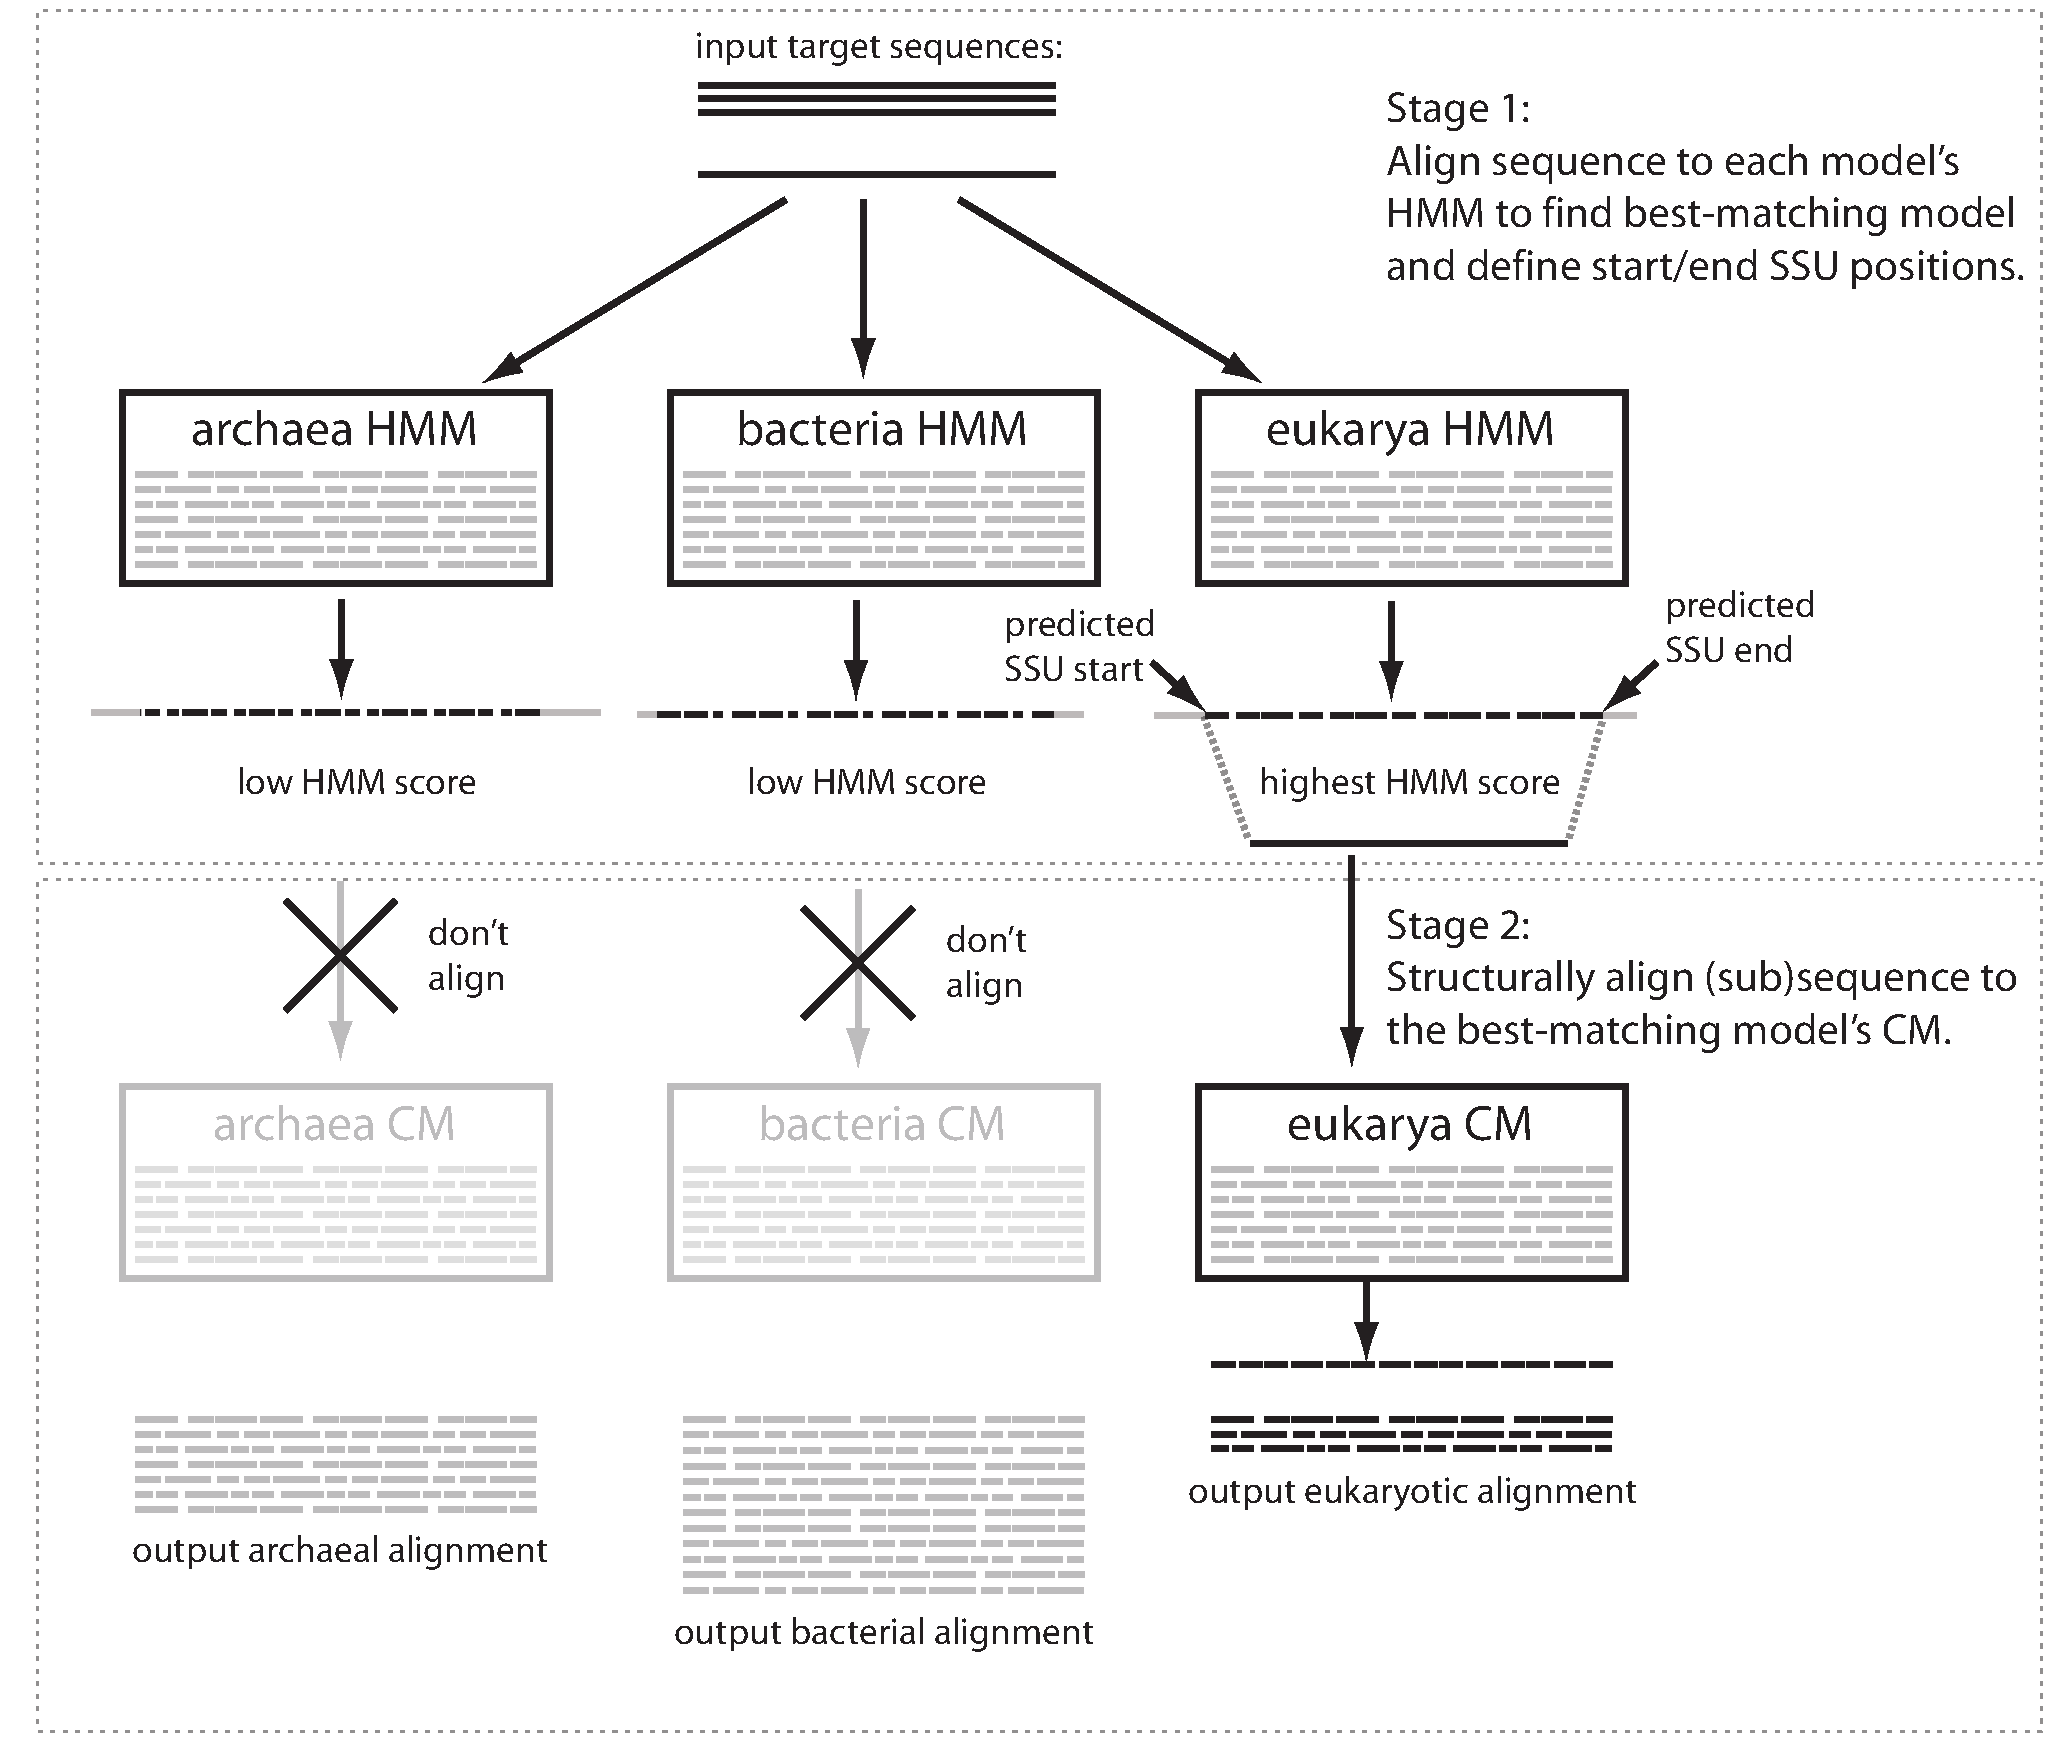
\includegraphics[width=6.5in]{Figures/ssualign-schematic}
  \end{center}
\caption{\textbf{Schematic of the \prog{ssu-align} alignment
    pipeline.} Unaligned target sequences are input to the
  program. In stage 1, each sequence is independently aligned
  using only primary sequence scoring to each of $N$ HMMs (by
  default, $N$ is 3), one built from each model in the input
  CM file. The model whose HMM alignment has the maximum bit
  score is the ``best-matching'' model for that sequence, in
  this example ``eukarya'' is the best-matching model. In
  stage 2, the unaligned (sub)sequence from the best-matching
  model's HMM alignment (potentially with some sequence
  trimmed off the ends) is aligned to the best-matching
  model's CM which scores both sequence and conserved
  secondary structure. The CM aligned target sequence is added
  to that model's output alignment. After all target sequences
  are processed, the program has output up to $N$ new
  structural alignments, one for each model that was the
  best-matching model for at least 1 target sequence.}
\label{fig:strategy}
\end{figure}

\newpage
% EPN, Thu Jun  3 08:04:50 2010
% NOTE: this install section was created by taking the first half of
% the HMMER3 installation section and the second half of the Infernal
% installation sections, glueing them together and making the
% necessary changes: substituting file names, adding text and removing
% parts that either don't apply, or don't work in SSU-ALIGN.

\section{Installation}
\label{sec:install}

\subsection{Quick installation instructions}
Download the source tarball (\prog{ssu-align.tar.gz}) from 
\url{http://selab.janelia.org/software.html}, or directly from 
\url{ftp://selab.janelia.org/software/ssu-align/ssu-align-0.1.tar.gz}; \\
untar; and change into the newly created directory \prog{ssu-align-0.1}:

\user{wget ftp://selab.janelia.org/pub/software/ssu-align/ssu-align-0.1.tar.gz}\\
\user{tar xf ssu-align-0.1.tar.gz}\\
\user{cd ssu-align-0.1}

Configure for your system, and build the programs:

\user{./configure}\\
\user{make}

Run the automated testsuite. This is optional. It takes about 10
minutes, and all these tests should pass:

\user{make check}

\begin{comment}
At this point, the programs are in the \prog{src} subdirectory, the
\prog{infernal/src} subdirectory and the
\prog{infernal/easel/miniapps} subdirectory. The
user's guide (this document) is in the \\ 
\prog{documentation/userguide}
subdirectory. The man pages are in the \prog{documentation/manpages}
subdirectory. You can manually move or copy all of these to
appropriate locations if you want. You will want the programs to be in
your \$PATH. 
\end{comment}

Install the man pages and programs in system-wide
directories:

\user{make install}

By default, programs are installed in \prog{/usr/local/bin}, man
pages in \prog{/usr/local/man/man1}, and data files and a \sft{perl}
module required by the programs are placed in 
\prog{/usr/local/share/ssu-align-0.1}. You might need special
privileges to write to \prog{/usr/local}. (You may need to execute
\prog{sudo make install}). You can change \prog{/usr/local} to any
directory you want using the \prog{./configure --prefix} option, as in
\prog{./configure --prefix /the/directory/you/want}.

After installing, you'll see the following:

\begin{sreoutput}
===============
SSU-ALIGN built
===============

The files "setup.ssu-align.bash" and "setup.ssu-align.csh" have been created.
If you use the bash shell, type "source setup.ssu-align.bash; rehash".
If you use the C shell, type "source setup.ssu-align.csh; rehash".
This will update your environment for this session.

To update your environment upon every login, you should
add the three lines:

export PATH="$PATH:/usr/local/bin"
export MANPATH="$MANPATH:/usr/local/share/man"
export SSUALIGNDIR="/usr/local/share/ssu-align-0.1"

to the ".bashrc" file in your home directory

or

setenv PATH "$PATH:/usr/local/bin"
setenv MANPATH "$MANPATH:/usr/local/share/man"
setenv SSUALIGNDIR "/usr/local/share/ssu-align-0.1"

to the ".cshrc" file in your home directory

To determine which shell you use, type:

echo $SHELL

If you prefer to manually update your environment variables,
be sure to make the following changes:

1. Add /usr/local/bin to your PATH variable
2. Add /usr/local/share/man to your MANPATH variable
3. Set $SSUALIGNDIR as /usr/local/share/ssu-align-0.1
\end{sreoutput}

Follow these instructions to update your environment. You'll 
want to both update the current session and add the three lines
indicated above to your \prog{.bashrc} or \prog{.cshrc} file in your
home directory so your environment is updated for every subsequent
session. 
\newpage

For instance, if you use the bash shell you'd do:

\user{source setup.ssu-align.bash}

to set up the environment for the current session only. You'd then go
to your \prog{.bashrc} file in your home directory (e.g.
\prog{Users/nawrockie/.bashrc}) and add the three lines: 

\prog{export PATH="\$PATH:/usr/local/bin"}

\prog{export MANPATH="\$MANPATH:/usr/local/share/man"}

\prog{export SSUALIGNDIR="/usr/local/share/ssu-align-0.1"}

Note that these will only work for the current configuration (that is,
they'll be different if you change the installation locations with
\prog{--prefix} or something like it). After doing this, you can test
if your environment is setup correctly by checking the following two
commands: 


\user{which ssu-align} 

should return the path to the \prog{ssu-align} script you
just installed (\prog{/usr/local/bin/ssu-align} by default), and

\user{echo \$SSUALIGNDIR}

should return the path to the your data directory
(\prog{/usr/local/share/ssu-align-0.1} by default).

That's it. You can keep reading if you want to know more about
customizing a \sft{ssu-align} installation, or you can skip ahead to
section~\ref{sec:tutorial}, the tutorial.

\subsection{More detailed installation notes}

The six main programs in the \software{ssu-align} package:
\prog{ssu-align}, \prog{ssu-build}, \prog{ssu-draw}, \prog{ssu-mask},\\
\prog{ssu-merge} and \prog{ssu-prep} are \sft{perl} scripts. The
package depends on, and includes, \sft{infernal} 
which itself includes \sft{hmmer} and the \sft{easel} sequence analysis
library; all of which are distributed as ANSI C source code. 

\sft{ssu-align} is designed to be built and used on UNIX platforms. It
is developed mainly on Intel GNU/Linux systems and Mac OS, and
intermittently tested on a variety of other UNIX platforms. It is not
currently tested on Microsoft Windows, but it should work there; it
should be possible to build it on any platform with an ANSI C
compiler. The software itself is vanilla POSIX-compliant ANSI C and
\sft{perl}. You may need to work around the configuration scripts and
Makefiles to get it built on a non-UNIX platform.

The GNU configure script that comes with \software{ssu-align} has a
number of options. You can see them all by doing:

\user{./configure --help}

Be warned that some of these options (such as \prog{--enable-mpi}) will
\emph{not} affect \sft{ssu-align} performance. These options affect only how
\sft{infernal} or \sft{hmmer} is built underneath \sft{ssu-align},
but have no impact on the toplevel \sft{ssu-align} programs. 

All customizations can and should be done at the \prog{./configure}
command line, unless you're a guru delving into the details of the
source code.

\subsubsection{Setting installation targets}

The most important options are those that let you set the installation
directories for \prog{make install} to be appropriate to your system.
What you need to know is that \software{ssu-align} installs three types
of files: programs, man pages, and data files. It installs the programs in
\prog{--bindir} (which defaults to \prog{/usr/local/bin}), the man pages in the
\prog{man1} subdirectory of \prog{--mandir} (default
\prog{/usr/local/man}) and the data files in a newly created
subdirectory \prog{ssu-align-0.1} of \prog{--datadir} (which
defaults to \prog{/usr/local/share}. Thus, say you want
\prog{make install} to install programs in \prog{/usr/bioprogs/bin}, man pages in
\prog{/usr/share/man/man1} and data files in \prog{/usr/share/ssu-align-0.1};
you would configure with:

\noindent \prog{> ./configure --mandir=/usr/share/man --bindir=/usr/bioprogs/bin --datatdir=/usr/share}

That's really all you need to know, since \software{ssu-align} installs
so few files. But just so you know; GNU configure is very flexible,
and has shortcuts that accomodates several standard conventions for
where programs get installed. One common strategy is to install all
files under one directory, like the default \prog{/usr/local}. To
change this prefix to something else, say \prog{/usr/mylocal}
(so that programs go in \prog{/usr/mylocal/bin}, man pages in
\prog{/usr/mylocal/man/man1}, and data files in
\prog{/usr/mylocal/share/ssu-align-0.1}), you can use the
\prog{--prefix} option:

\user{./configure --prefix=/usr/mylocal}

\begin{comment}
% EPREFIX doesn't work with ssu-align's configure; not sure why
Another common strategy (especially in multiplatform environments) is
to put programs in an architecture-specific directory like
\prog{/usr/share/Linux/bin} while keeping man pages in a shared,
architecture-independent directory like \prog{/usr/share/man/man1}.
GNU configure uses \prog{--exec-prefix} to set the path to
architecture dependent files; normally it defaults to being the same
as \prog{--prefix}. You could change this, for example, by:

\user{./configure --prefix=/usr/share --exec-prefix=/usr/share/Linux}\\
\end{comment}

In summary, a complete list of the \prog{./configure} installation
options that affect \software{ssu-align}:

\begin{tabular}{lll}
Option                       & Meaning                         & Default\\ \hline
\prog{--prefix=PREFIX}       & all files                       & \prog{/usr/local} \\
\prog{--bindir=DIR}          & programs                        & PREFIX/bin/\\
\prog{--mandir=DIR}          & man pages                       & PREFIX/man/\\
\prog{--datadir=DIR}         & data files                      & PREFIX/share/\\
\end{tabular}


\subsubsection{Setting compiler and compiler flags}

By default, \prog{configure} searches first for the GNU C compiler
\prog{gcc}, and if that is not found, for a compiler called \prog{cc}. 
This can be overridden by specifying your compiler with the \prog{CC}
environment variable.

By default, the compiler's optimization flags are set to
\prog{-g -O3} for \prog{gcc}, or \prog{-g} for other compilers.
This can be overridden by specifying optimization flags with the
\prog{CFLAGS} environment variable. 

For example, to use an Intel C compiler in
\prog{/usr/intel/ia32/bin/icc} with 
optimization flags \prog{-O3 -ipo}, you would do:

\user{env CC=/usr/intel/ia32/bin/icc CFLAGS="-O3 -ipo" ./configure}

which is the one-line shorthand for:

\user{setenv CC     /usr/intel/ia32/bin/icc}\\
\user{setenv CFLAGS "-O3 -ipo"}\\
\user{./configure}

If you are using a non-GNU compiler, you will almost certainly want to
set \prog{CFLAGS} to some sensible optimization flags for your
platform and compiler. The \prog{-g} default generated unoptimized
code. At a minimum, turn on your compiler's default optimizations with
\prog{CFLAGS=-O}.

\begin{comment}
% This is unchanged from infernal
\subsection{Example configuration}

The Intel GNU/Linux version installed at Janelia Farm is configured as
follows:

{\scriptuser{env CFLAGS="-O3" ./configure --enable-mpi --enable-lfs --prefix=/usr/local/infernal-1}}
\end{comment}

% This is copied and modified from the HMMER3 installation section of
% its user's guide
\subsection{Makefile targets}

\begin{sreitems}{\emprog{distclean}}
\item[\emprog{all}]
  Builds everything. Same as just saying \prog{make}.

\item[\emprog{check}]
  Runs the automated test for SSU-ALIGN.

\item[\emprog{clean}]
  Removes all files generated by compilation (by
  \prog{make}). Configuration (files generated by
  \prog{./configure}) is preserved.

\item[\emprog{distclean}]
  Removes all files generated by configuration (by \prog{./configure})
  and by compilation (by \prog{make}). 

  Note that if you want to make a new configuration you
  should do a \prog{make distclean} (rather than a \prog{make
    clean}), to be sure old configuration files aren't used
  accidentally.
\end{sreitems}


\newpage
\section{Background: alignment using profiles}

\subsection{What is a profile probabilistic model?}

\begin{comment}
Profile probabilistic models are statistical models of a sequence
family that include \emph{position-specific} information about which
residues are 

For our purposes here it is 

Examples include profile hidden Markov models, commonly used
for protein sequence homology search and implemented in some widely
used software packages such as \software{HMMER} (CITE). 
\end{comment}

\subsection{Software implementing profile probabilistic models}

\subsection{Nearest-neighbor based methods}

\subsection{The motivation for \textsc{SSU-align}}

\subsection{Alignment confidence estimates}

\subsection{Bit scores}


\newpage
\section{Basic tutorial: defining and aligning SSU sequences using \textsc{SSU-align}}

Here is a tutorial walk-through of a small project with
\software{SSUalign}. This tutorial shows how to use the program for
it's most basic and fundamental purpose, creating multiple
alignments of SSU rRNA sequences. 

\subsection{Files used in this tutorial}

The subdirectory \prog{/tutorial-basic} in the \software{SSU-align}
contains the files used in this tutorial, they are:

  \begin{sreitems}{}
  \item[\prog{ssu.default.0p1.cm}] A covariance model (CM) file that
    defines five SSU rRNA CMs: an archael model, a bacterial model, a
    choloroplast model, a eukaryotic model and a metazoan
    mitrochondria model. These are the five default models used by
    \textsc{SSU-align}. These models are explained in section 4.
  \item[\prog{rocks.fa}] SSU rRNA sequences from an environmental
    survey sequencing project of microbes living in the pore space of
    rocks in the Rocky Mountains by J.J. Walker and Norm Pace
    \cite{Walker07}. 
  \item[\prog{1p0.params}] A file containing paths to
    \textsc{infernal} executable files that \textsc{SSU-align} needs
    to run. You will likely need to change these paths to point to
    where you've installed the \prog{cmsearch} and \prog{cmalign}
    programs (these are created in 'infernal-1.0/src/' after building
    \textsc{infernal} version 1.0 with 'sh ./configure; make;') and
    the \prog{esl-sfetch} program (which is created in
    'infernal-1.0/easel/miniapps/' after building \textsc{infernal}
    version 1.0).
  \end{sreitems}

Create a new directory that you can work in, and copy all the files in
\prog{tutorial-basic} there. I'll assume for the following examples that
you've installed the \software{SSU-align} script in your path; if not,
you'll need to give a complete path name to the script
(e.g. something like
\newline
\prog{/usr/people/nawrocki/ssualign/src/ssu-align} 
instead of just \prog{ssu-align}).

\subsection{An example run of \textsc{ssu-align}}

The file \prog{rocks.fa} contains 588 SSU sequences
\cite{Walker07}. \textsc{SSU-align} is designed to create structural
alignments of SSU sequences from studies like this one. To run it,
execute the following command:

\user{ssu-align ssu.default.0p1.cm rocks.fa myrun 1p0.params}\\

The program will print a header describing the program version used,
command used, current date, and some other information. Then it will
begin stage 1:

\begin{sreoutput}
# ssu-align :: define and align SSU rRNA sequences
# SSU-ALIGN 0.1 (June 2009)
# Copyright (C) 2009 HHMI Janelia Farm Research Campus
# Freely distributed under the GNU General Public License (GPLv3)
# - - - - - - - - - - - - - - - - - - - - - - - - - - - - - - - - - - - -
# command: /groups/eddy/home/nawrockie/ssualign/ssu-align ssu.default.1p0.cm rocks.fa myrun 1p0.params
# date:    Wed Jun 17 05:37:27 2009
#
# Stage 1: Determining SSU start/end positions and best matching models.
\end{sreoutput}

In stage 1, the program scans the input sequences with each of the
five models in the CM file \prog{ssu.default.0p1.cm}. This has two
purposes.  First, it classifies each sequence by determining which
model gives each sequence the highest primary sequence-based alignment
score using a profile HMM. Secondly, it defines the start and end
points of the SSU sequences.

Stage 1 takes about 5 minutes on this dataset. When it finishes you'll
see: 

\begin{sreoutput}
# Stage 1: Determining SSU start/end positions and best matching models.
#
# output file name               description                                   
# -----------------------------  ----------------------------------------------
  myrun.tab                      locations/scores of hits defined by HMM(s)
  myrun.Archaea.hits.list        list of sequences to align with Archaea CM
  myrun.Archaea.hits.fa               48 sequences to align with Archaea CM
  myrun.Bacteria.hits.list       list of sequences to align with Bacteria CM
  myrun.Bacteria.hits.fa             341 sequences to align with Bacteria CM
  myrun.Chloroplast.hits.list    list of sequences to align with Chloroplast CM
  myrun.Chloroplast.hits.fa          199 sequences to align with Chloroplast CM
\end{sreoutput}

This lists and briefly describes the 7 new files the script created in
a newly created subdirectory of the current working dir called
\prog{myrun/}. The first file \prog{myrun.tab} is output from
\textsc{infernal}'s \prog{cmsearch} program. The other 6 files are
model-specific, two for each model that was the best-matching model to
at least 1 sequence in the input target sequence file
\prog{rocks.fa}. The \prog{.hits.list} suffixed files contain a list
of the sequences that match best to the model, and the \prog{.hits.fa}
suffixed files are those actual sequences. There were no sequences
that best-matched the eukaryotic model or the metazoan mitochondria
model, so no model-specific files were created for those two models.
Each of these file types is explained in more detail below in the
``Description of output files'' section, but for now we'll continue
following the output of our example \prog{ssu-align} run.

The program will now proceed to stage 2, the alignment stage. This
stage serially progresses through each model that was the
best-matching model for at least 1 sequence and uses the model to
align best-matching sequences. The alignments are computed by scoring
a combination of both sequence and secondary structure conservation,
as opposed to the scoring in stage 1 which only used sequence
conservation. When the alignment to each model finishes, a list of two
newly created files will appear on the screen. For this example,
alignment to all three models takes about 6 minutes. When it finishes
you'll see:

\begin{sreoutput}
#
# Stage 2: Aligning each sequence to it's best matching model.
#
# output file name               description
# -----------------------------  ----------------------------------------------
  myrun.Archaea.cmalign.stk      Archaea alignment
  myrun.Archaea.cmalign          Archaea cmalign output
  myrun.Bacteria.cmalign.stk     Bacteria alignment
  myrun.Bacteria.cmalign         Bacteria cmalign output
  myrun.Chloroplast.cmalign.stk  Chloroplast alignment
  myrun.Chloroplast.cmalign      Chloroplast cmalign output
  myrun.scores                   list of CM/HMM scores for each sequence
  myrun.log                      log file (*this* text printed to stdout)
#
# All output files created in directory ./myrun/
#
# CPU time (search):     00:04:35
# CPU time (alignment):  00:06:19
# CPU time (total):      00:10:55
\end{sreoutput}

The actual alignments are the \prog{.cmalign.stk} suffixed
files. These were created by the \textsc{infernal} program
\prog{cmalign}. The \prog{cmalign} output is in the \prog{.cmalign}
suffixed files.  As in stage 1, these files were created in
the \prog{./myrun/} subdirectory. 

\subsection{Description of output files}

Now we'll go through each of the output file types
created by\prog{ssu-align}, starting with the alignments.

Take a look at the archaeal alignment we just created in
\prog{myrun/myrun.Archaea.cmalign.stk}. 

This alignment includes consensus secondary structure annotation and
is in \emph{Stockholm format}. 
Stockholm format, the native alignment format used by \software{hmmer} and
\software{Infernal} and the \database{Pfam} and \database{Rfam}
databases, is documented in detail in the \software{Infernal} User's
Guide which is included in this distribution in
\prog{infernal/documentation/userguide.pdf}.

For now, what you need to know about the key features of the alignment file is:
\begin{itemize}

\item The alignment is in an interleaved format, like other
  common alignment file formats such as \software{clustalw}.
  Lines consist of a name, followed by an aligned sequence;
  the alignment is split into blocks separated by blank lines.

\item Gaps are indicated by the characters ., \_, -, or \verb+~+.
  qNotice that the first few blocks of the alignment are 100% gaps.
  This is because the sequences in \prog{rocks.fa} are not full length
  SSU sequences, but rather partial sequences obtained using PCR
  primers that target well conserved regions within the SSU
  molecule. In this alignment you'll have to scroll down to about line
  1300 before you see an aligned residue.

\item Special lines starting with {\small\verb+#=GR+} followed by a
  sequence name and then {\small\verb+POST+} contain posterior
  probabilities for each aligned residue for the sequence they
  correspond to. These are confidence estimates in the correctness of
  the alignment.  The POSTX. row indicates the ’tens’ place of the
  confidence estimate while POST.X row indicates the ’ones’ place. So
  the confidence estimate for a residue with 9 in the POSTX. row, and
  7 in the POST.X row to two significant digits 97%. This means that
  if you sampled alignments from the posterior distribution of all
  possible alignments of this sequence to the model, about 97% of the
  time that residue would appear in that of the alignment. One special
  case: if the posterior probability is very nearly 100% (it’s
  difficult to be more precise on the exact percentage due to
  numerical precision issues) the annotated posterior values will be
  ``*'' characters in both the tens and one places. These confidence
  estimates can be used to mask the alignment to remove columns with
  significant fractions of ambiguously aligned residues as demonstrated
  in the next section.

\item A special line starting with {\small\verb+#=GC SS_cons+}
  indicates the secondary structure consensus. Gap characters annotate
  unpaired (single-stranded) columns. Base pairs are indicated by any
  of the following pairs: \verb+<>+, \verb+()+, \verb+[]+, or
  \verb+[]+.

\item A special \"RF\" line starting with {\small\verb+#=GC RF+}
  indicates the consensus, or ReFerence, model. Gaps in the RF line
  are \emph{insert} columns, where at least 1 sequence has at least 1
  inserted residue between two consensus positions. Uppercase residues
  in the RF line are well conserved positions in the model; lowercase
  residues are less well conserved.
\end{itemize}

\subsection{Creating secondary structure diagrams that display alignment statistics}

SSU rRNA alignments are large and difficult to view in a meaningful
way. \textsc{ssu-align} includes a program \prog{esl-ssudraw} for
creating secondary structure diagrams that display statistics of a
particular alignment on the consensus secondary structure used to
align the model. To use \prog{esl-ssudraw} requires a template
postscript file of the consensus secondary structure. The template
files for the 5 default \textsc{ssu-align} version 0.1 seed models are
included, but constructing these required a significant amount of
work, and creating your own templates for different models would be
difficult. 

Let's create a diagram that shows the information content of each
position of our newly created archaeal alignment:

\prog{esl-ssudraw 




To convert the alignment to fasta format that includes gaps, you can use the
\prog{scripts/stk2aln\_fa.pl} script. 

\subsection{Pruning the alignment based on probabilistic confidence
  estimates}


\newpage
\section{The SSU ribosomal RNA secondary structure models used by \textsc{ssu-align}}
\label{sect:models}

The profile probabilistic models of SSU rRNA in \textsc{ssu-align} are
derived from the alignments generated by Robin Gutell and colleagues
at the University of Texas Austin \cite{Cannone02}. There are 5 CM
files, each was constructed from a separate alignment from the
Comparative RNA Website as explained below.

\subsection{SSU rRNA data available from the Comparative RNA Website}

The Comparative RNA Website (CRW) is an extremely valuable for
sequence and structure data on many structural RNAs including small
subunit ribosomal RNA, large subunit ribosomal RNA, 5S and 5.8S
ribsomal RNA, group I and group II self-splicing introns. For the
purpose of building SSU rRNA CMs, the most relevant information
available from CRW is multiple alignments and individual secondary
structures that were determined using comparative analysis for a
subset of the sequences available in the alignments. 

TO DO.

\begin{comment}
\textsc{infernal} builds a CM from a consensus structure annotated
multiple sequence alignment. So, to use the CRW data I had to develop
a pipeline that mapped the individual structures onto the alignments
and then derived a consensus structure from the individual structures.

I decided to first extract only the sequences that had individual
structure information from the larger alignments, 

Because the unique feature of CM SSU alignment relative to other existing
methods is it's ability to take secondary structure into account
during alignment the most important information from CRW 

\textsc{infernal} builds sequence and structure profiles of an RNA
sequence family from a multiple alignment of 
\end{comment}

\subsection{Deriving consensus structure annotated \emph{seed} alignments from CRW data}

TO DO.

\subsection{Building CMs from seed alignments}

\textsc{infernal}'s \prog{cmbuild} program builds CM files from
consensus structure annotated alignments. \textsc{ssu-align} includes
the five default training alignments (named \prog{<family>.stk}, where
\prog{<family>} is either archaea, bacteria, chlorplast, eukarya or
metamito) as well as the five CMs resulting from them (named
\prog{<family>.cm}). (The metamito model is a metazoan mitochondria
model). The models were built using \prog{cmbuild} as
follows: 

\user{cmbuild --enone --gapthresh 0.8 archaea.cm archaea.stk}

\begin{comment}
The default behavior and parameters of \prog{cmbuild} have been
optimized to build CMs that are sensitive to remote homology detection
in homology search applications (the main application of CMs)
\cite{Nawrocki07}. But when building CMs for accurate SSU rRNA
alignment a few parameters can be tweaked to get better
performance. 
\end{comment}

MORE ON WHY THESE OPTIONS WERE USED.

\subsection{Seed alignment and model statistics} 

% stats from esl-alistat and cmbuild-1.0 on ssu5-0p1.stk
\begin{center}
\begin{tabular}{lrrrrrr}
        &           &           &           &           & average   & average  \\
model   & number of & consensus & alignment & number of & sequence  & pairwise \\
name    & sequences & length    & length    & basepairs & length    & identity \\ \hline
        &           &           &           &                       &          \\
archaea & 23        & 1508      & 1563      & 471       & 1485      & 81\%     \\
bacteria& 93        & 1582      & 1689      & 480       & 1527      & 80\%     \\
chloroplast& 18     & 1514      & 1693      & 449       & 1492      & 85\%     \\
eukarya  & 89       & 1881      & 2652      & 448       & 1800      & 79\%     \\ 
metamito & 55       &  996      & 1127      & 256       & 957       & 76\%     \\
\end{tabular}
\end{center}

\subsection{Secondary structure diagrams of seed alignments}

TO INCLUDE: HEATMAPS of the 5 models.

\begin{center}

\newpage
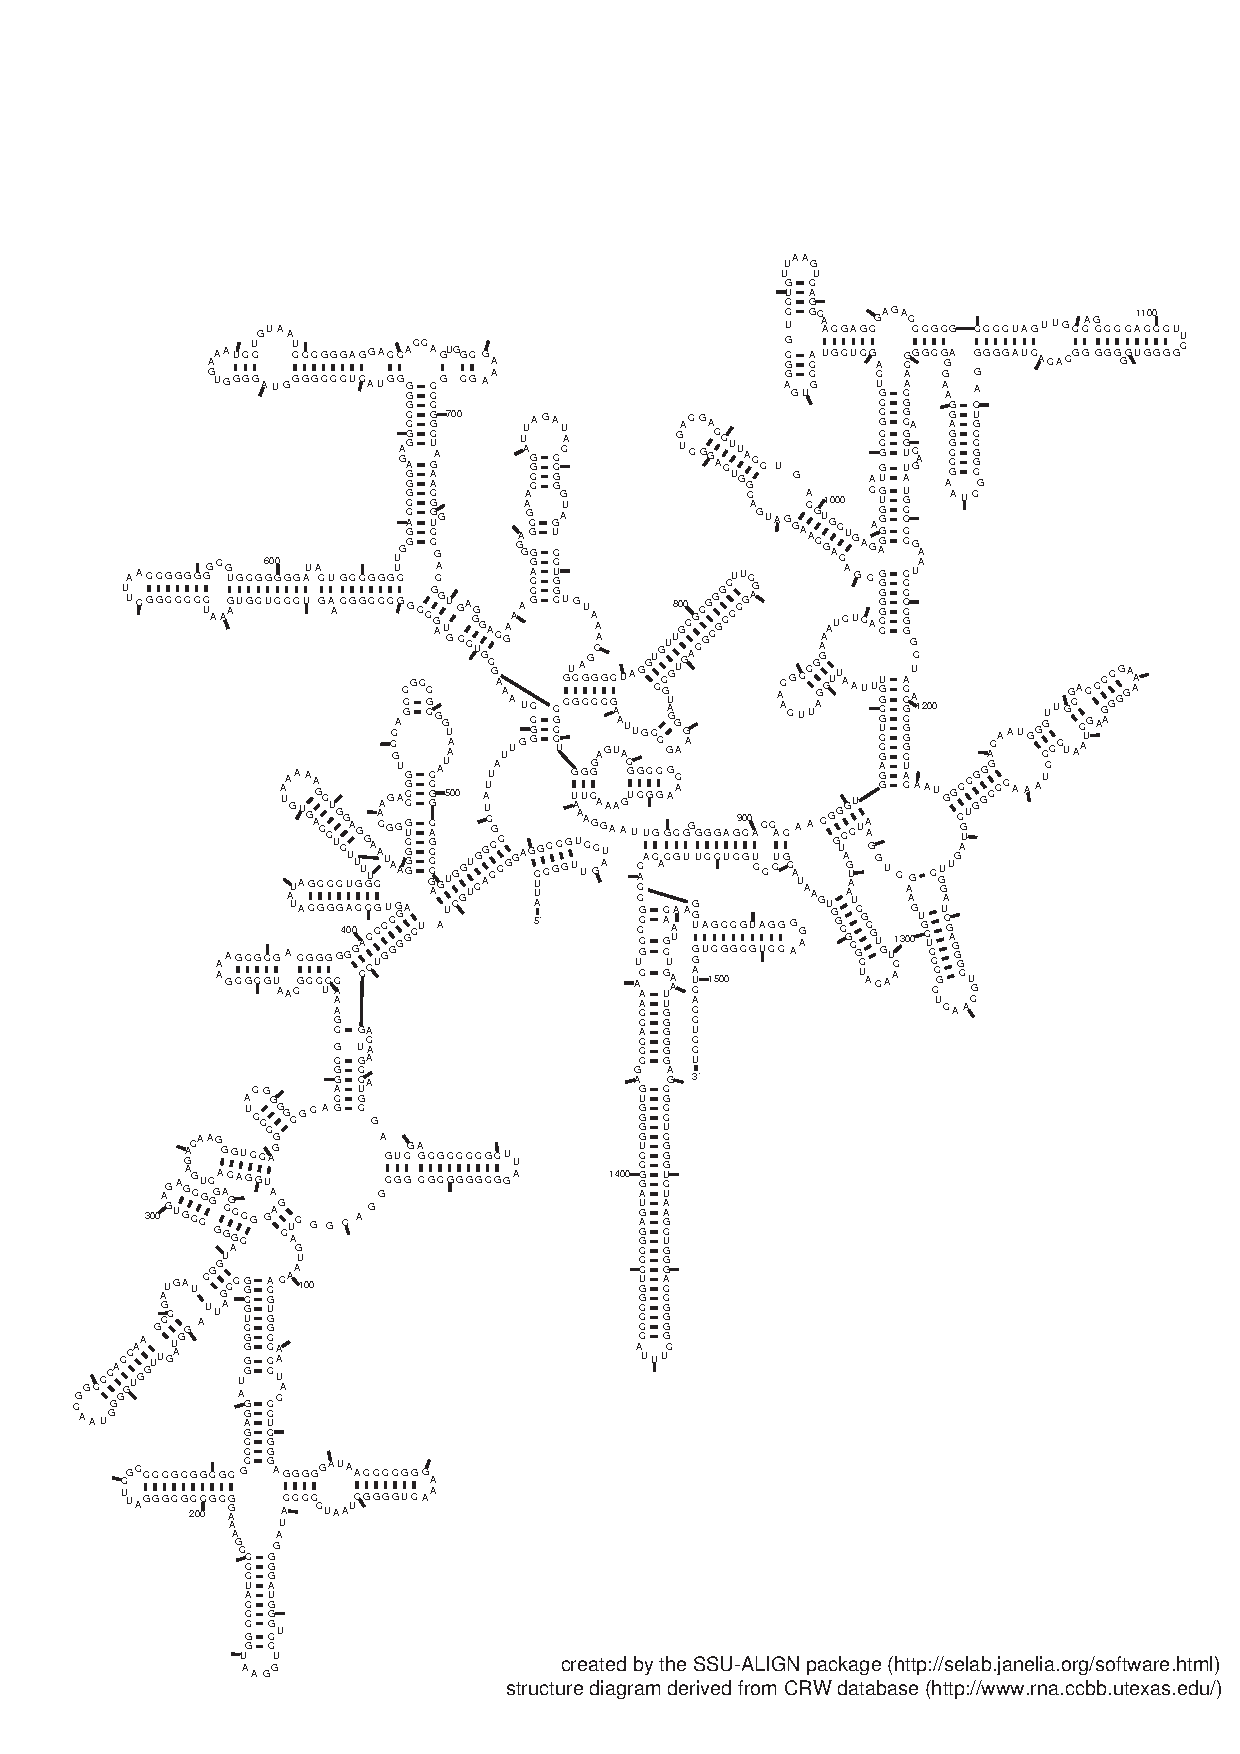
\includegraphics[height=8.5in]{../../seeds/ss-diagrams/archaea-0p1}

\newpage
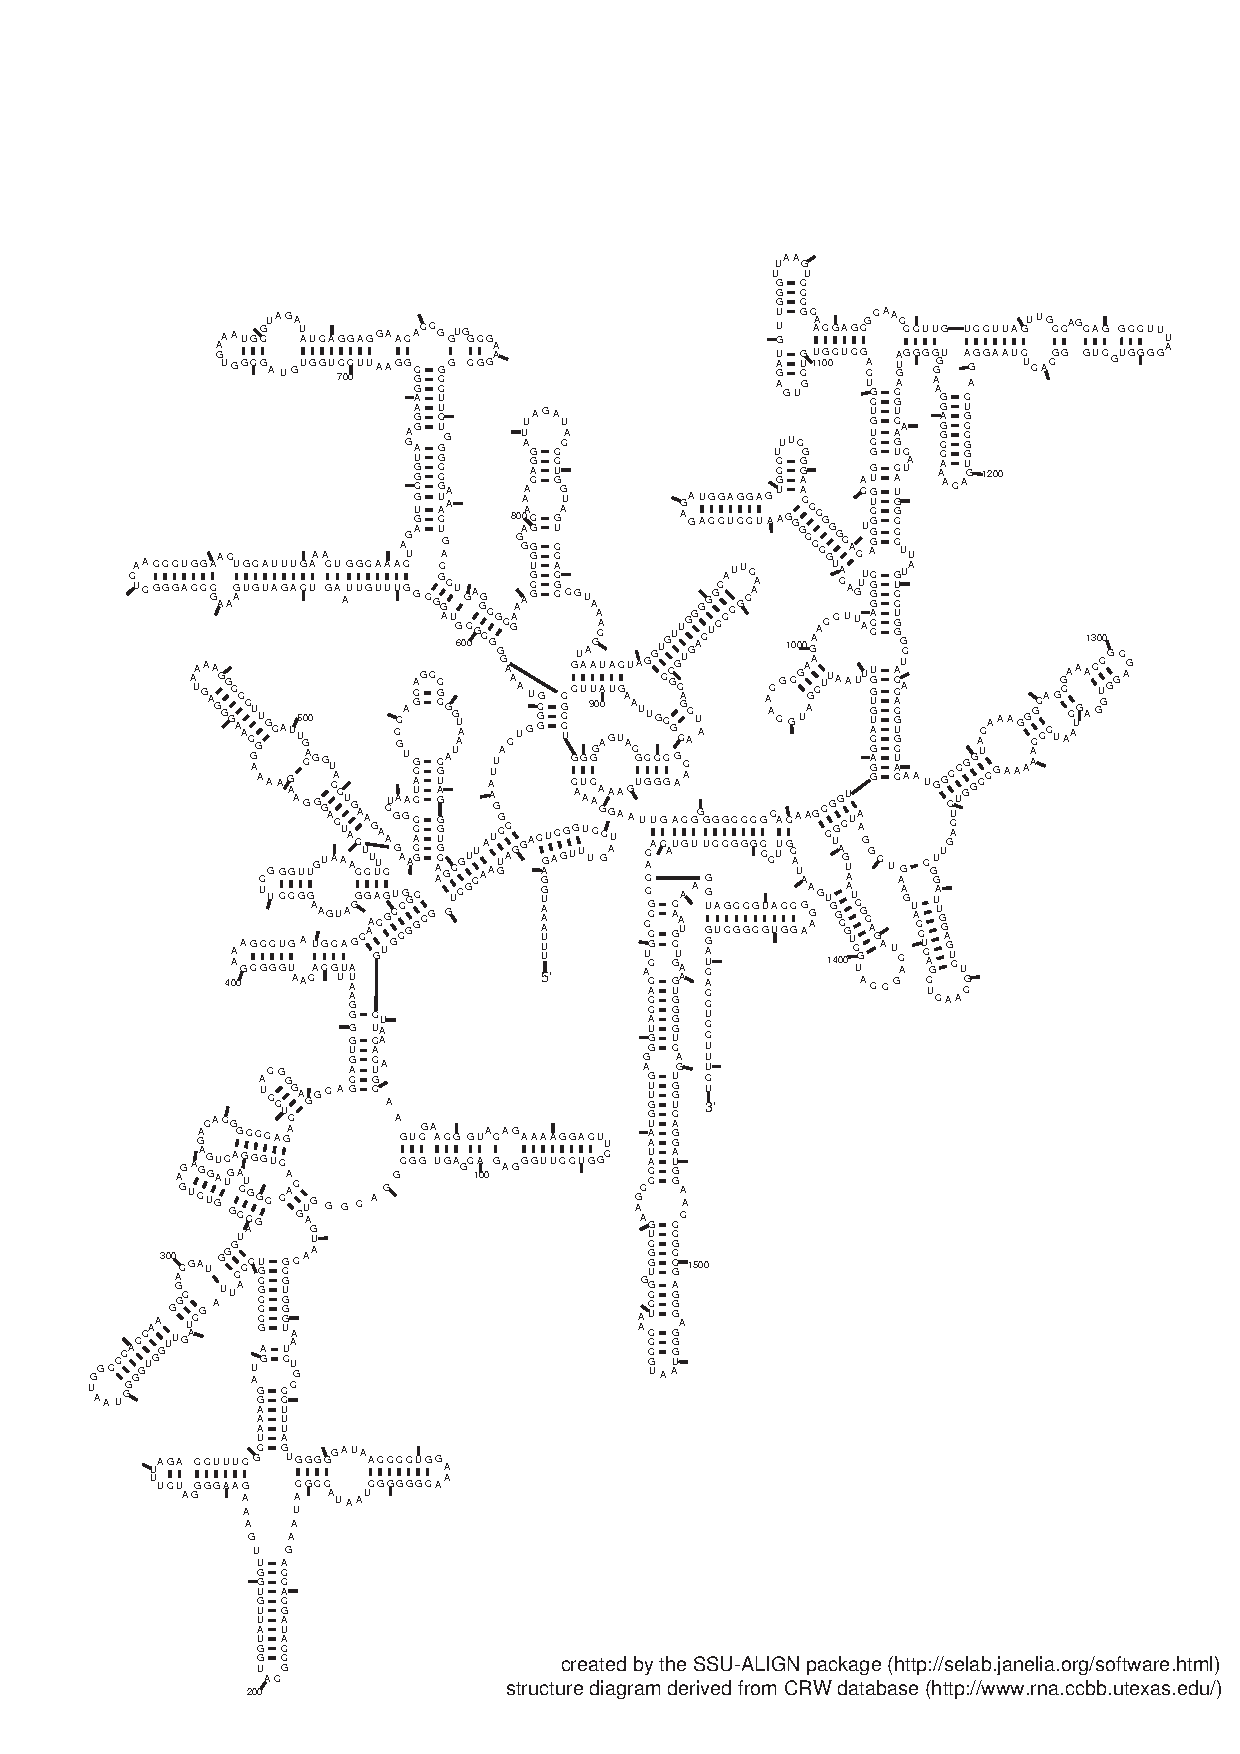
\includegraphics[height=8.5in]{../../seeds/ss-diagrams/bacteria-0p1}

\newpage
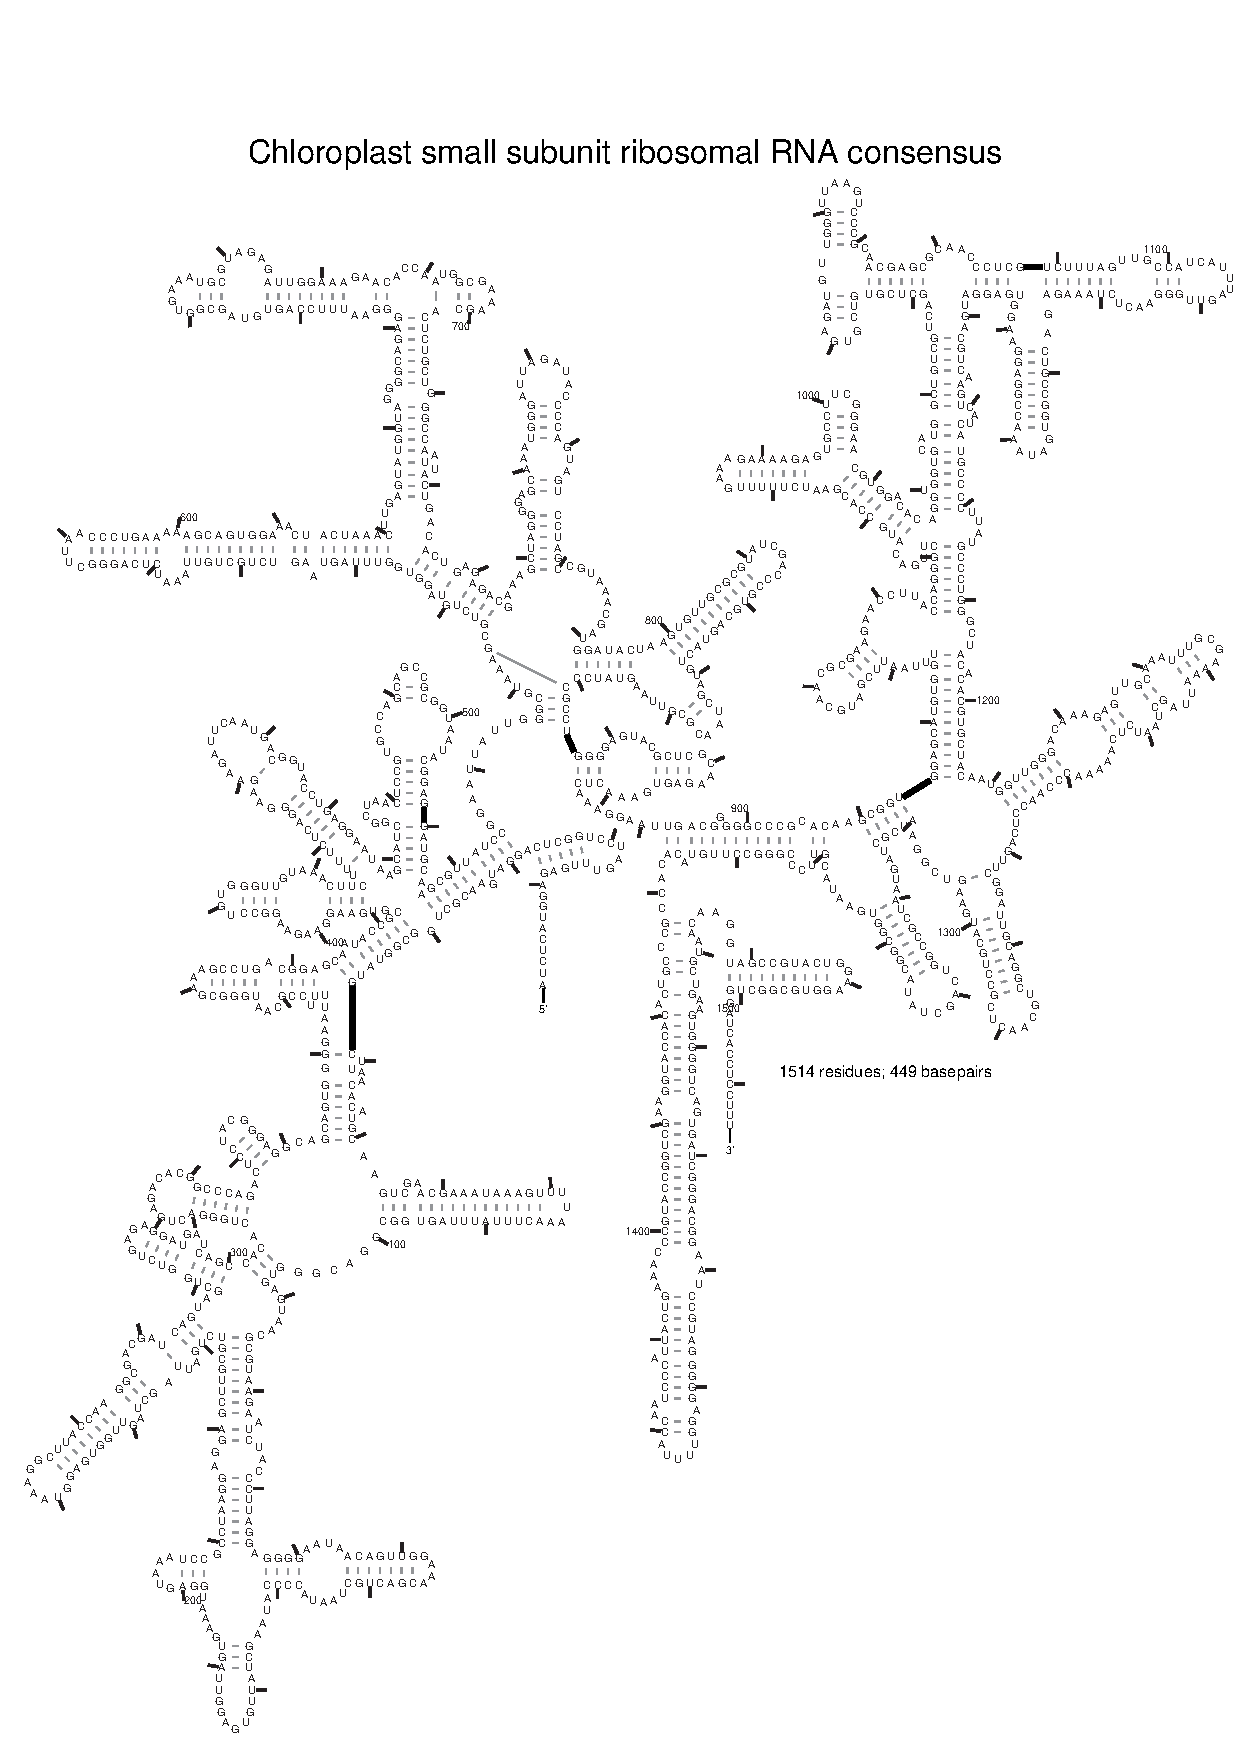
\includegraphics[height=8.5in]{../../seeds/ss-diagrams/chloroplast-0p1}

\newpage
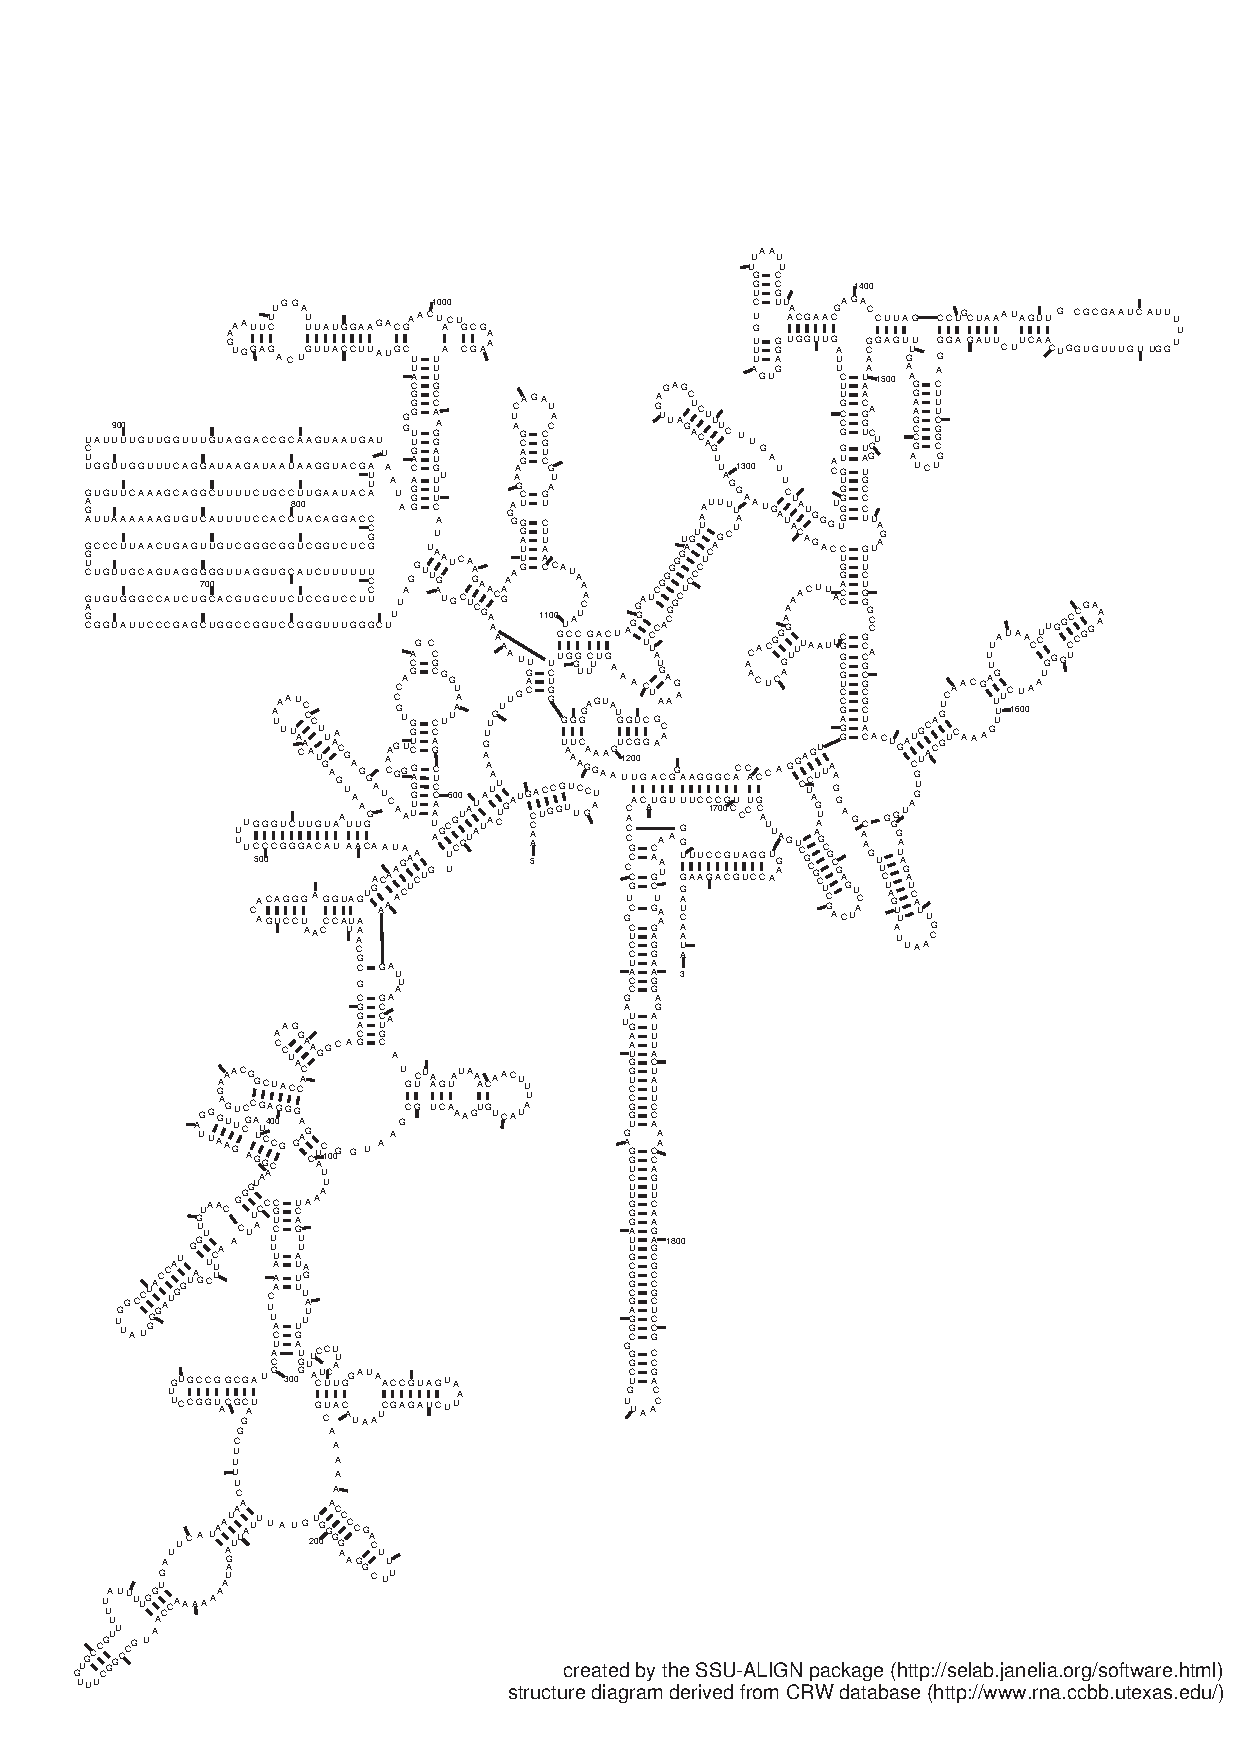
\includegraphics[height=8.5in]{../../seeds/ss-diagrams/eukarya-0p1}

\newpage
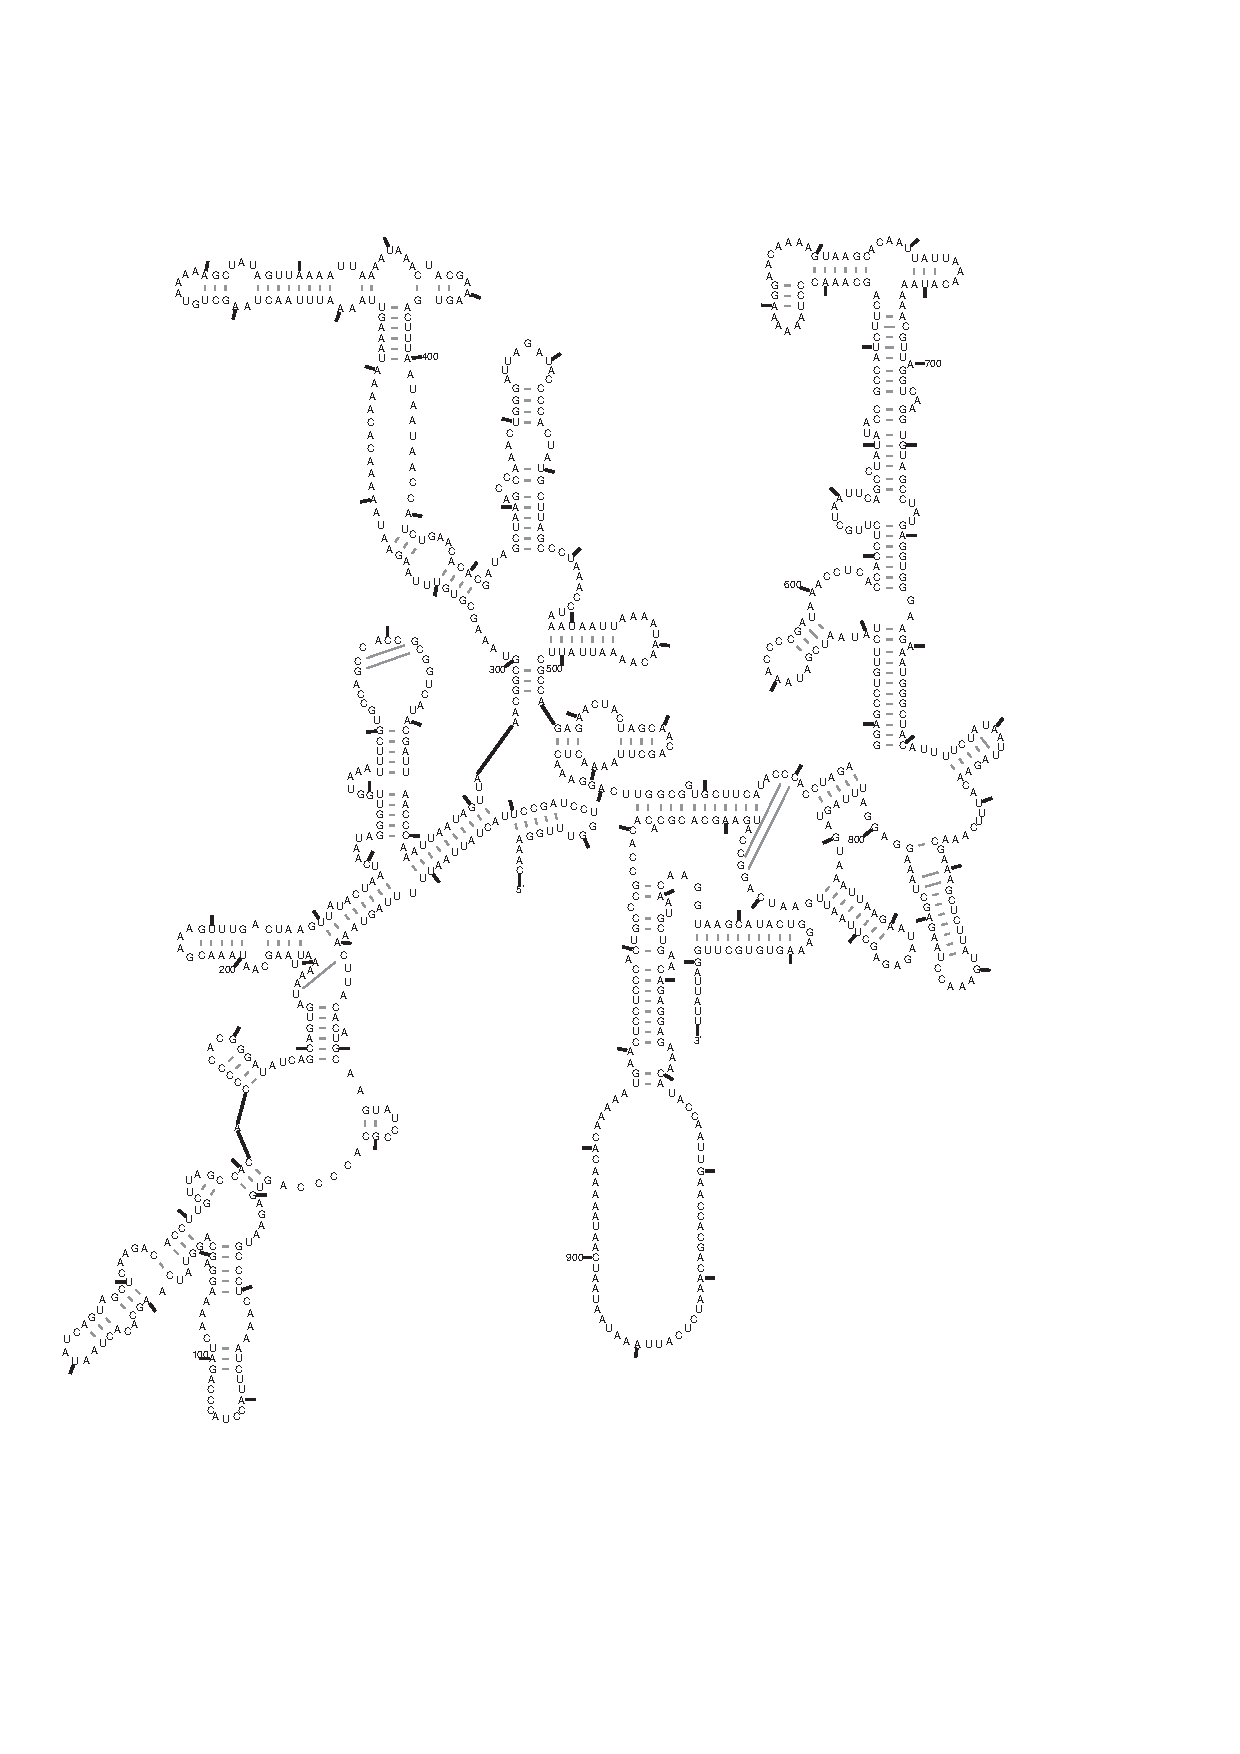
\includegraphics[height=8.5in]{../../seeds/ss-diagrams/metamito-0p1}

\end{center}

\begin{comment}
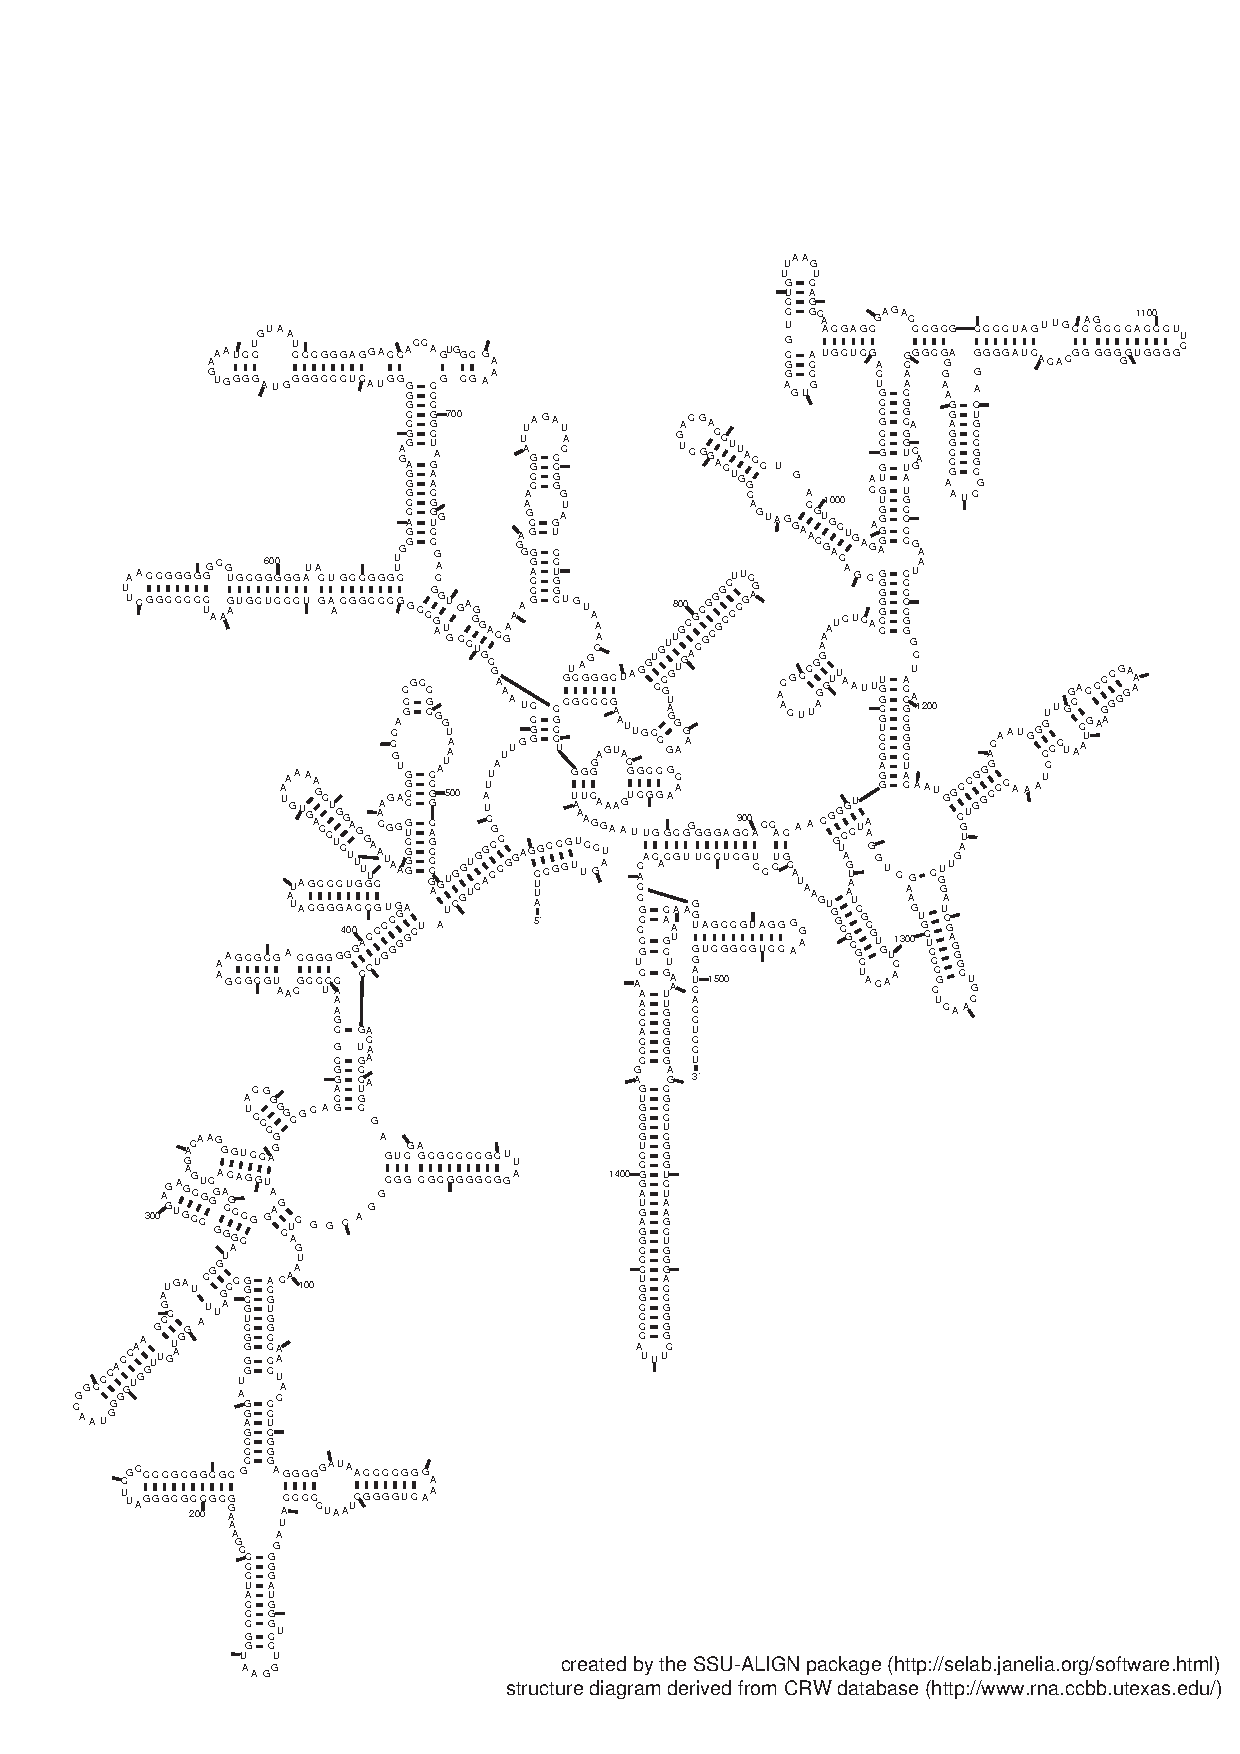
\includegraphics[height=8.5in]{../../seeds/ss-diagrams/archaea-0p1}
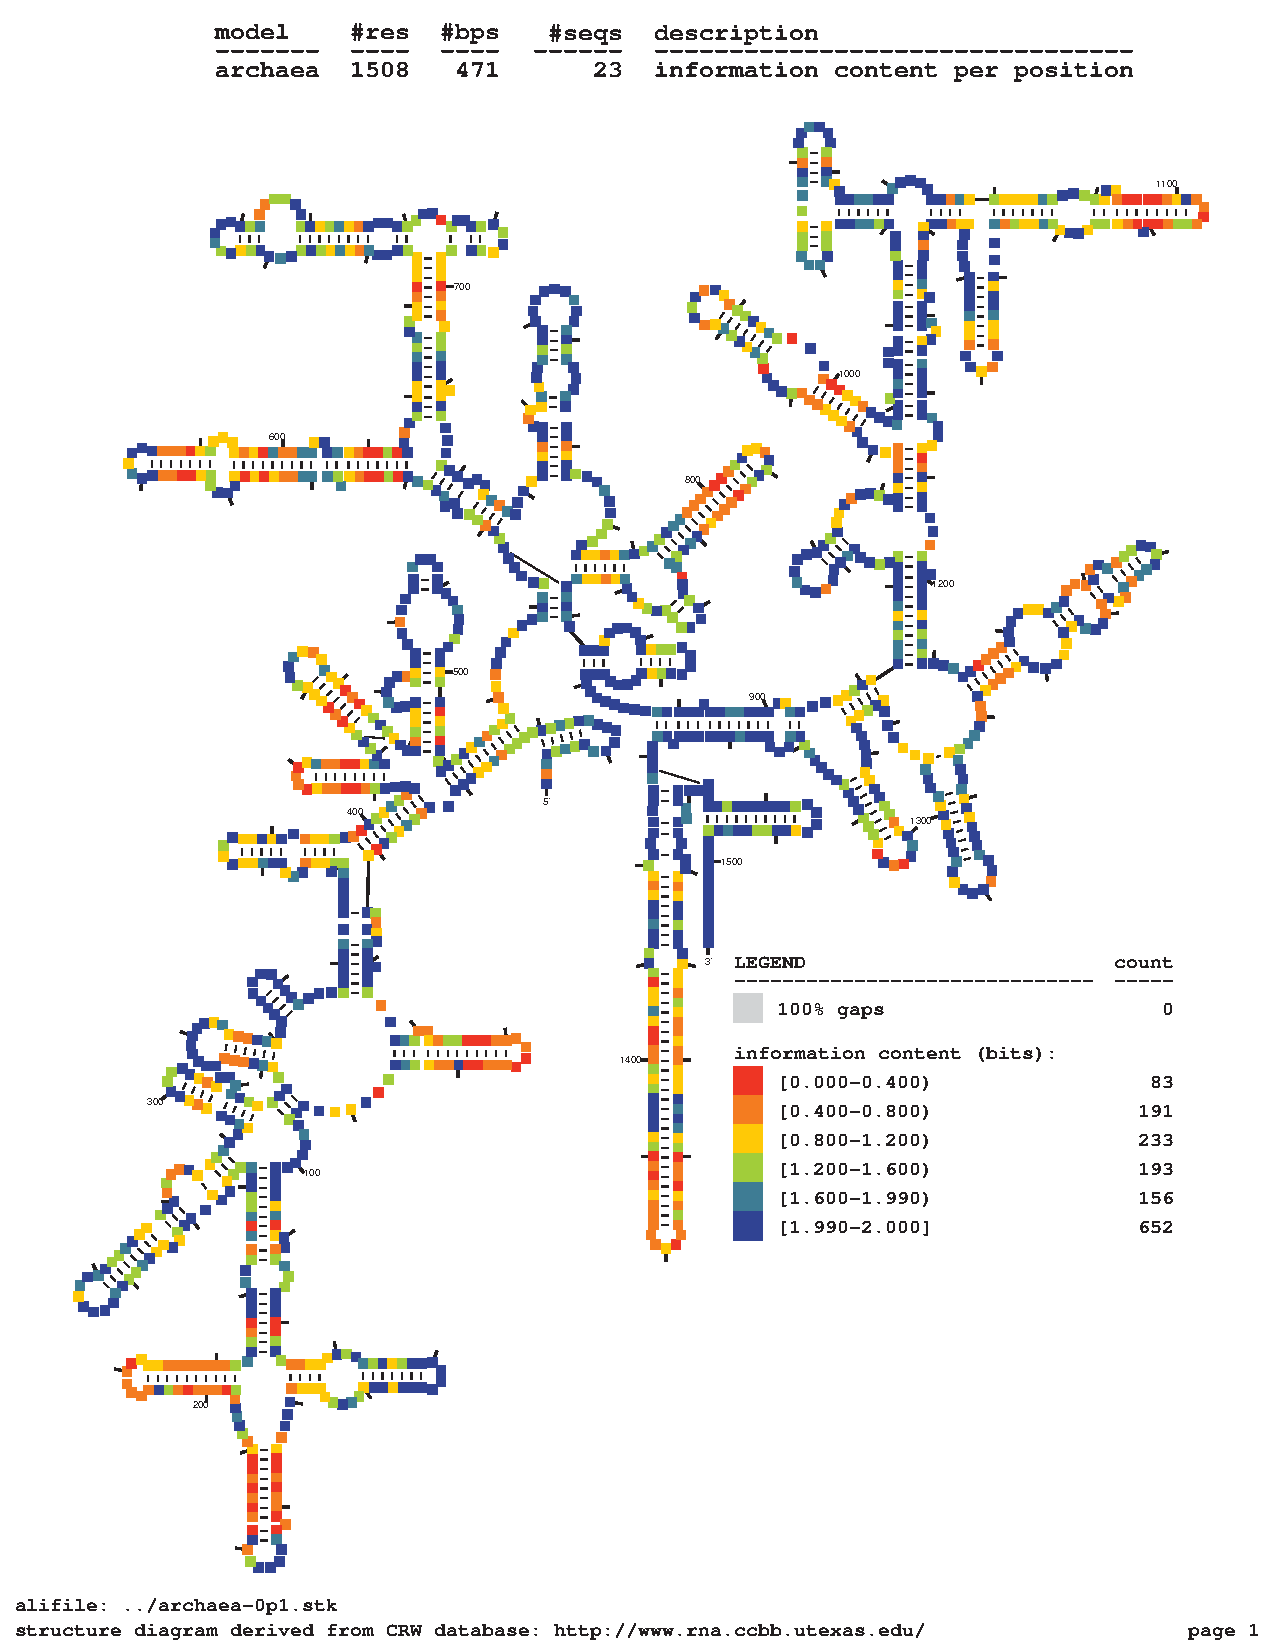
\includegraphics[height=8.5in]{../../seeds/ss-diagrams/archaea-0p1-info}
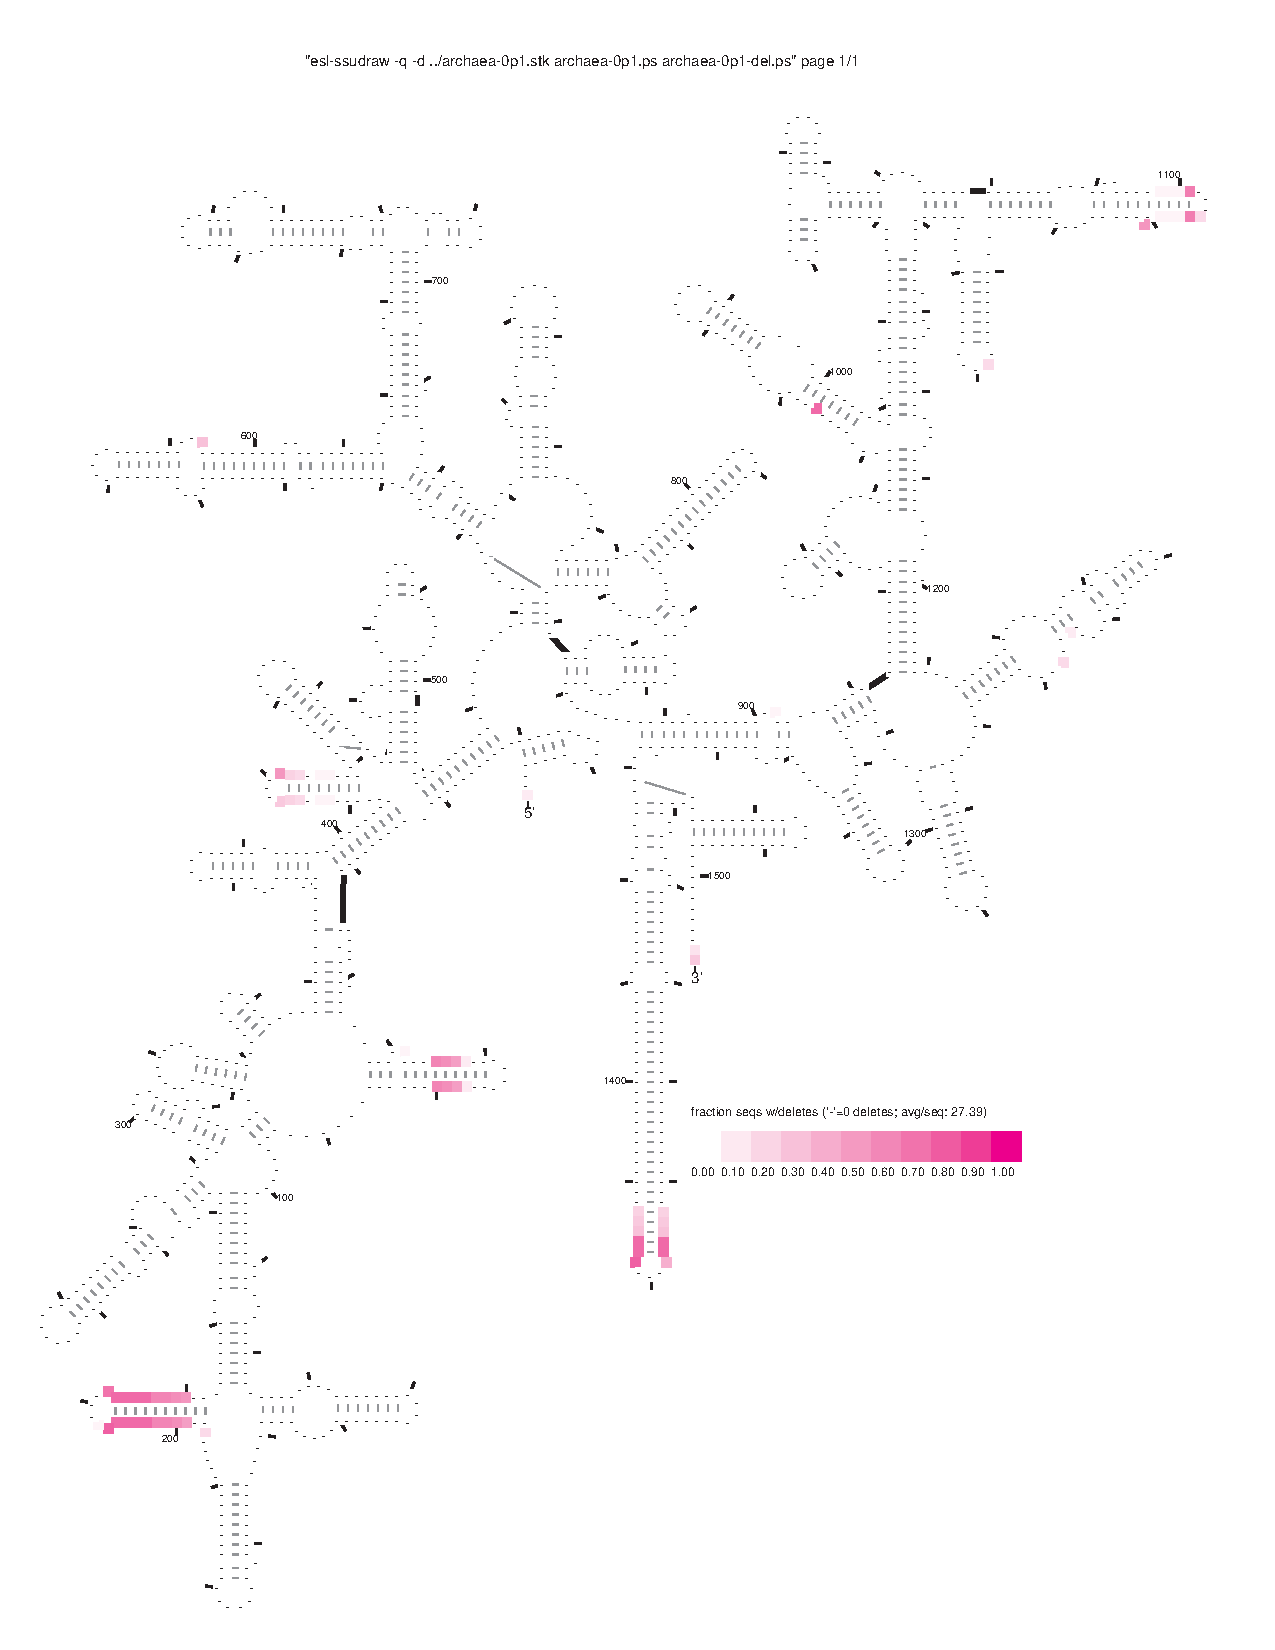
\includegraphics[height=8.5in]{../../seeds/ss-diagrams/archaea-0p1-del}
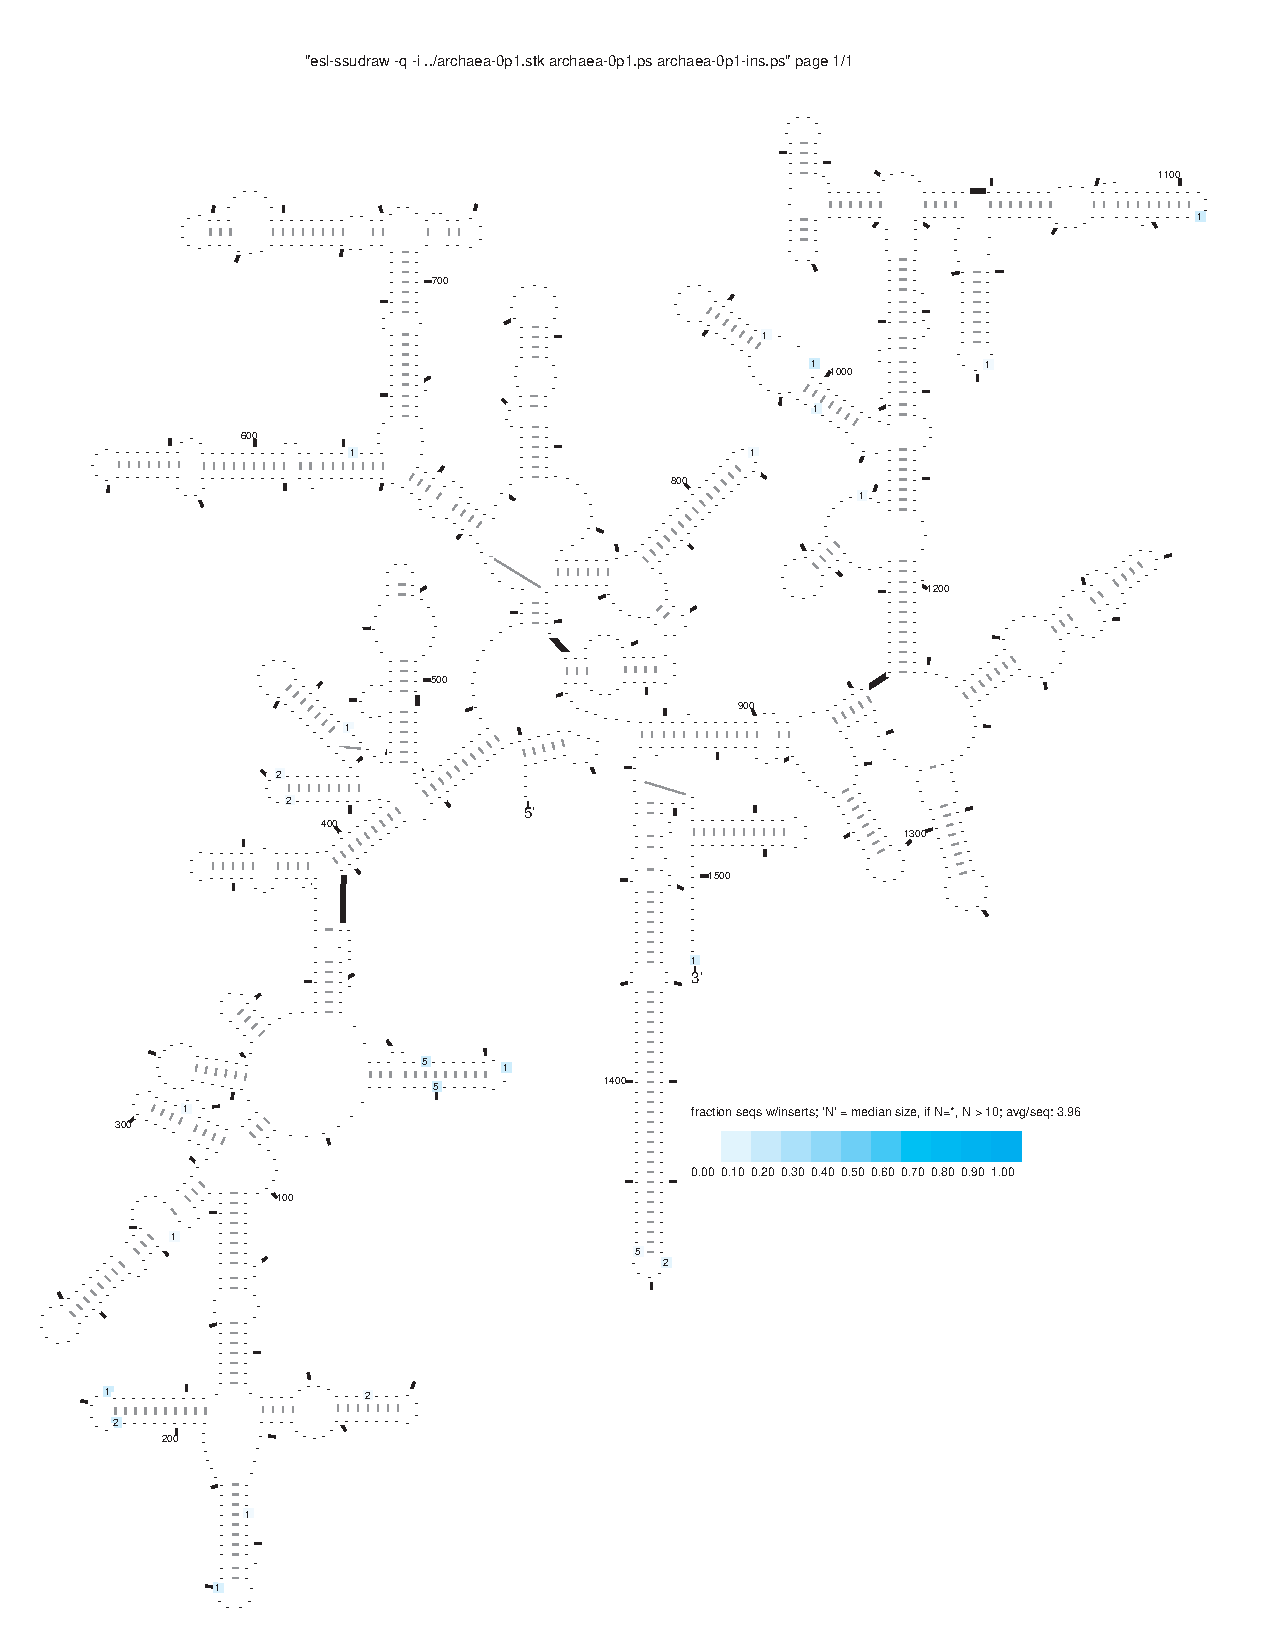
\includegraphics[height=8.5in]{../../seeds/ss-diagrams/archaea-0p1-ins}

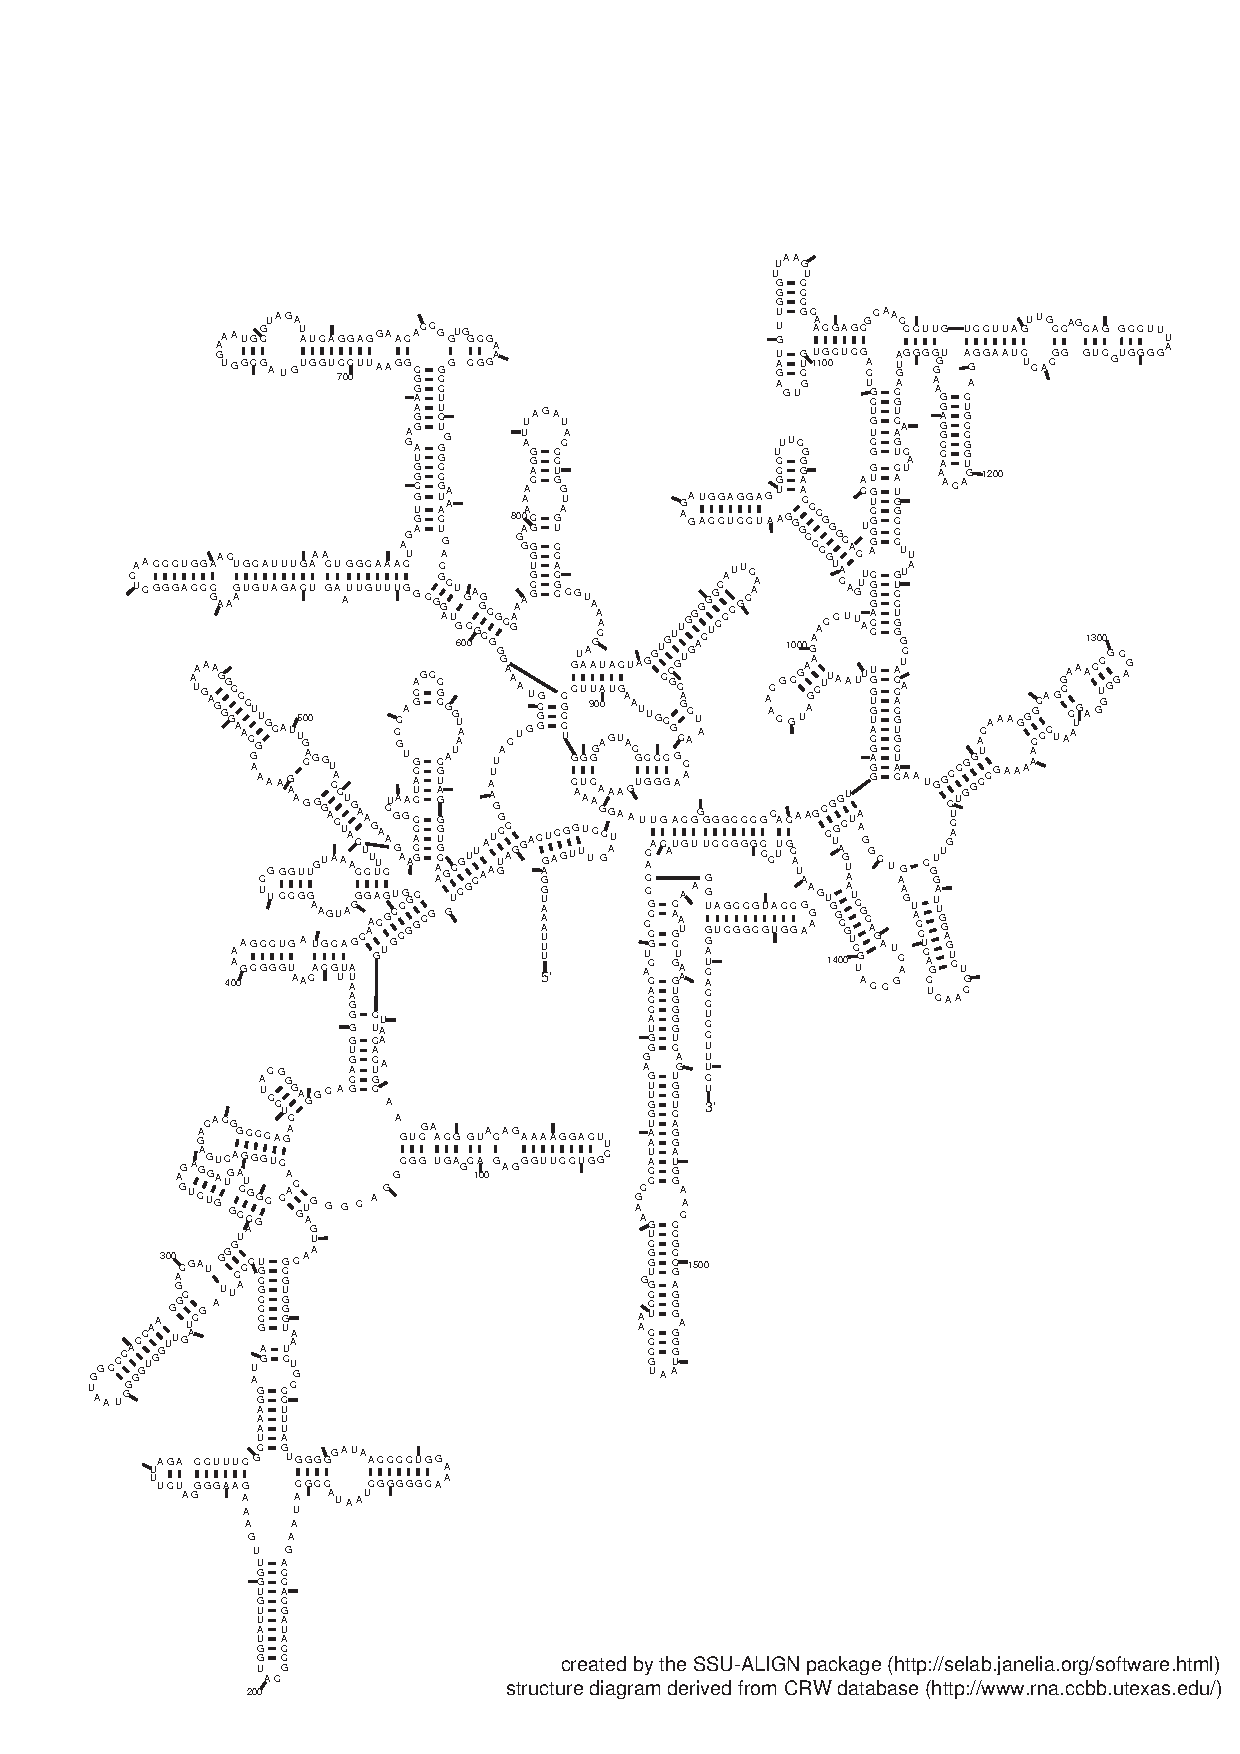
\includegraphics[height=8.5in]{../../seeds/ss-diagrams/bacteria-0p1}
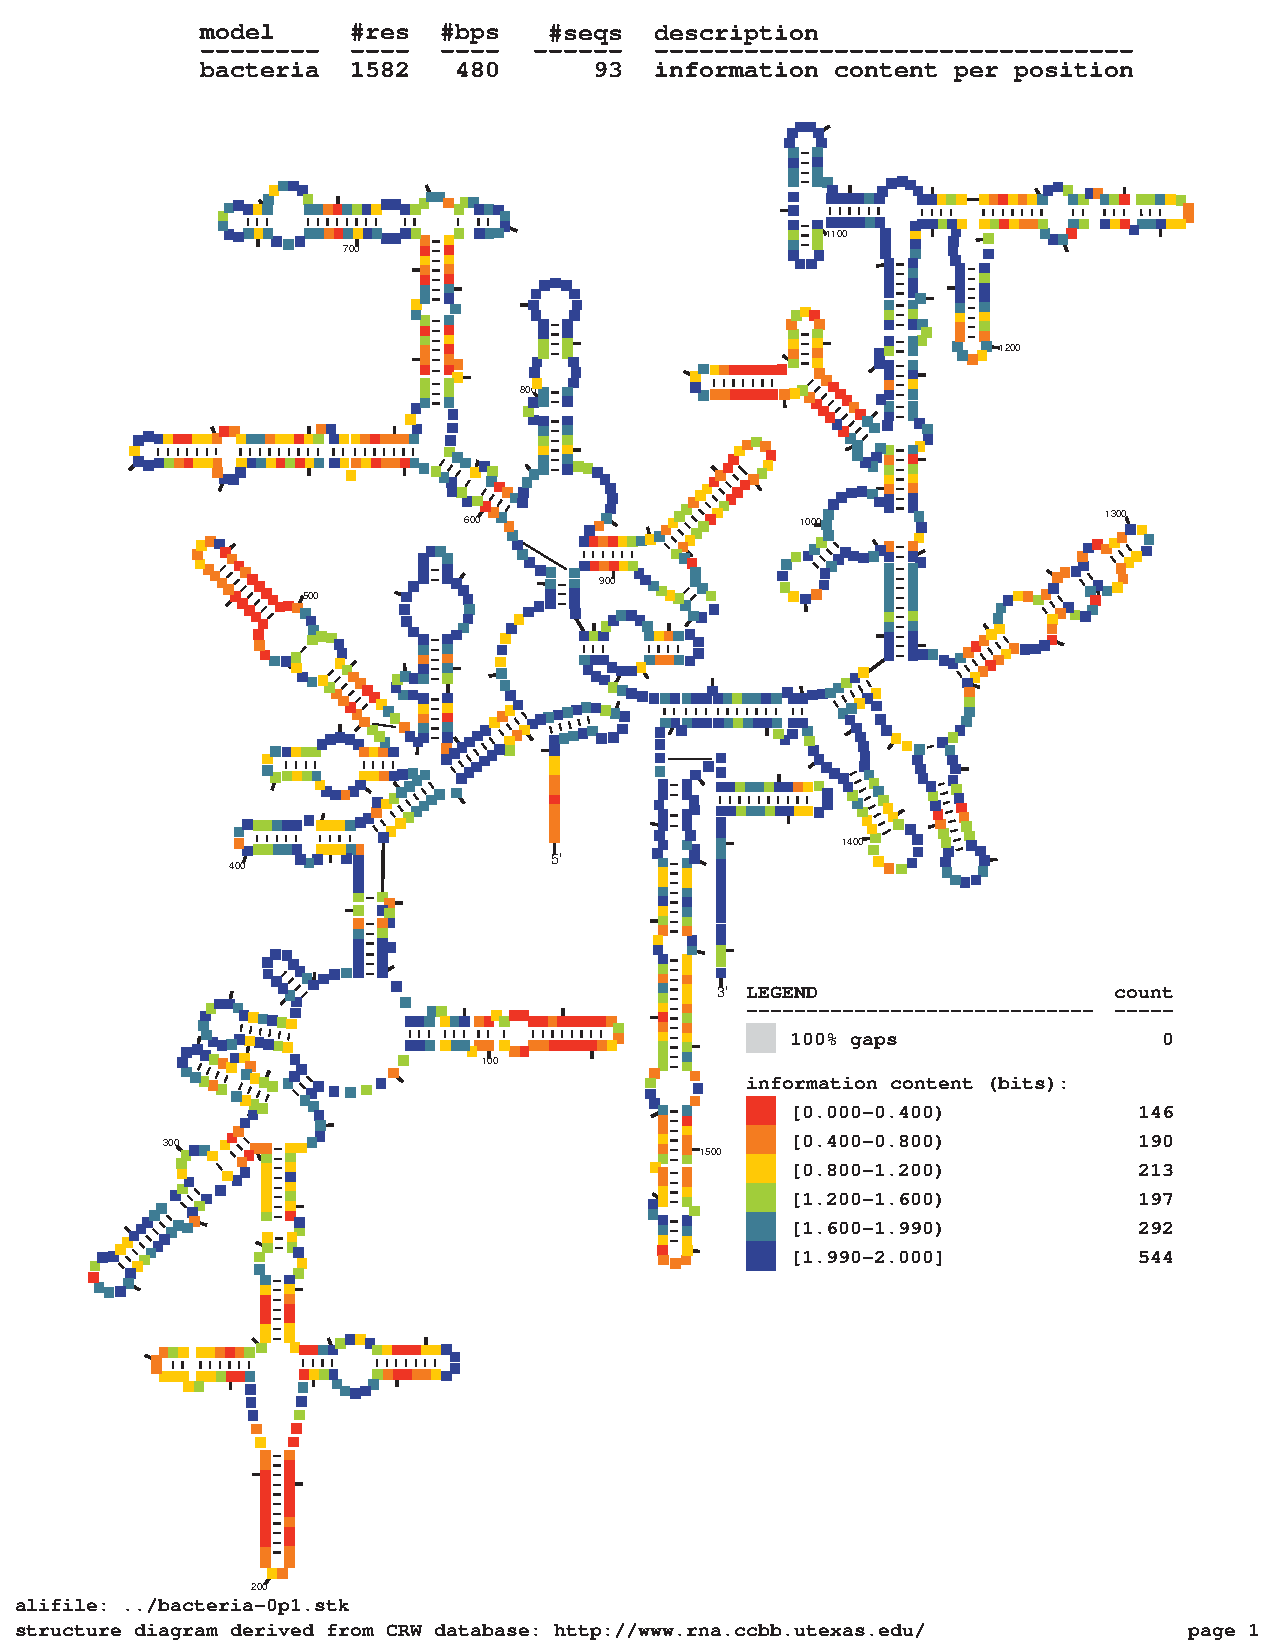
\includegraphics[height=8.5in]{../../seeds/ss-diagrams/bacteria-0p1-info}
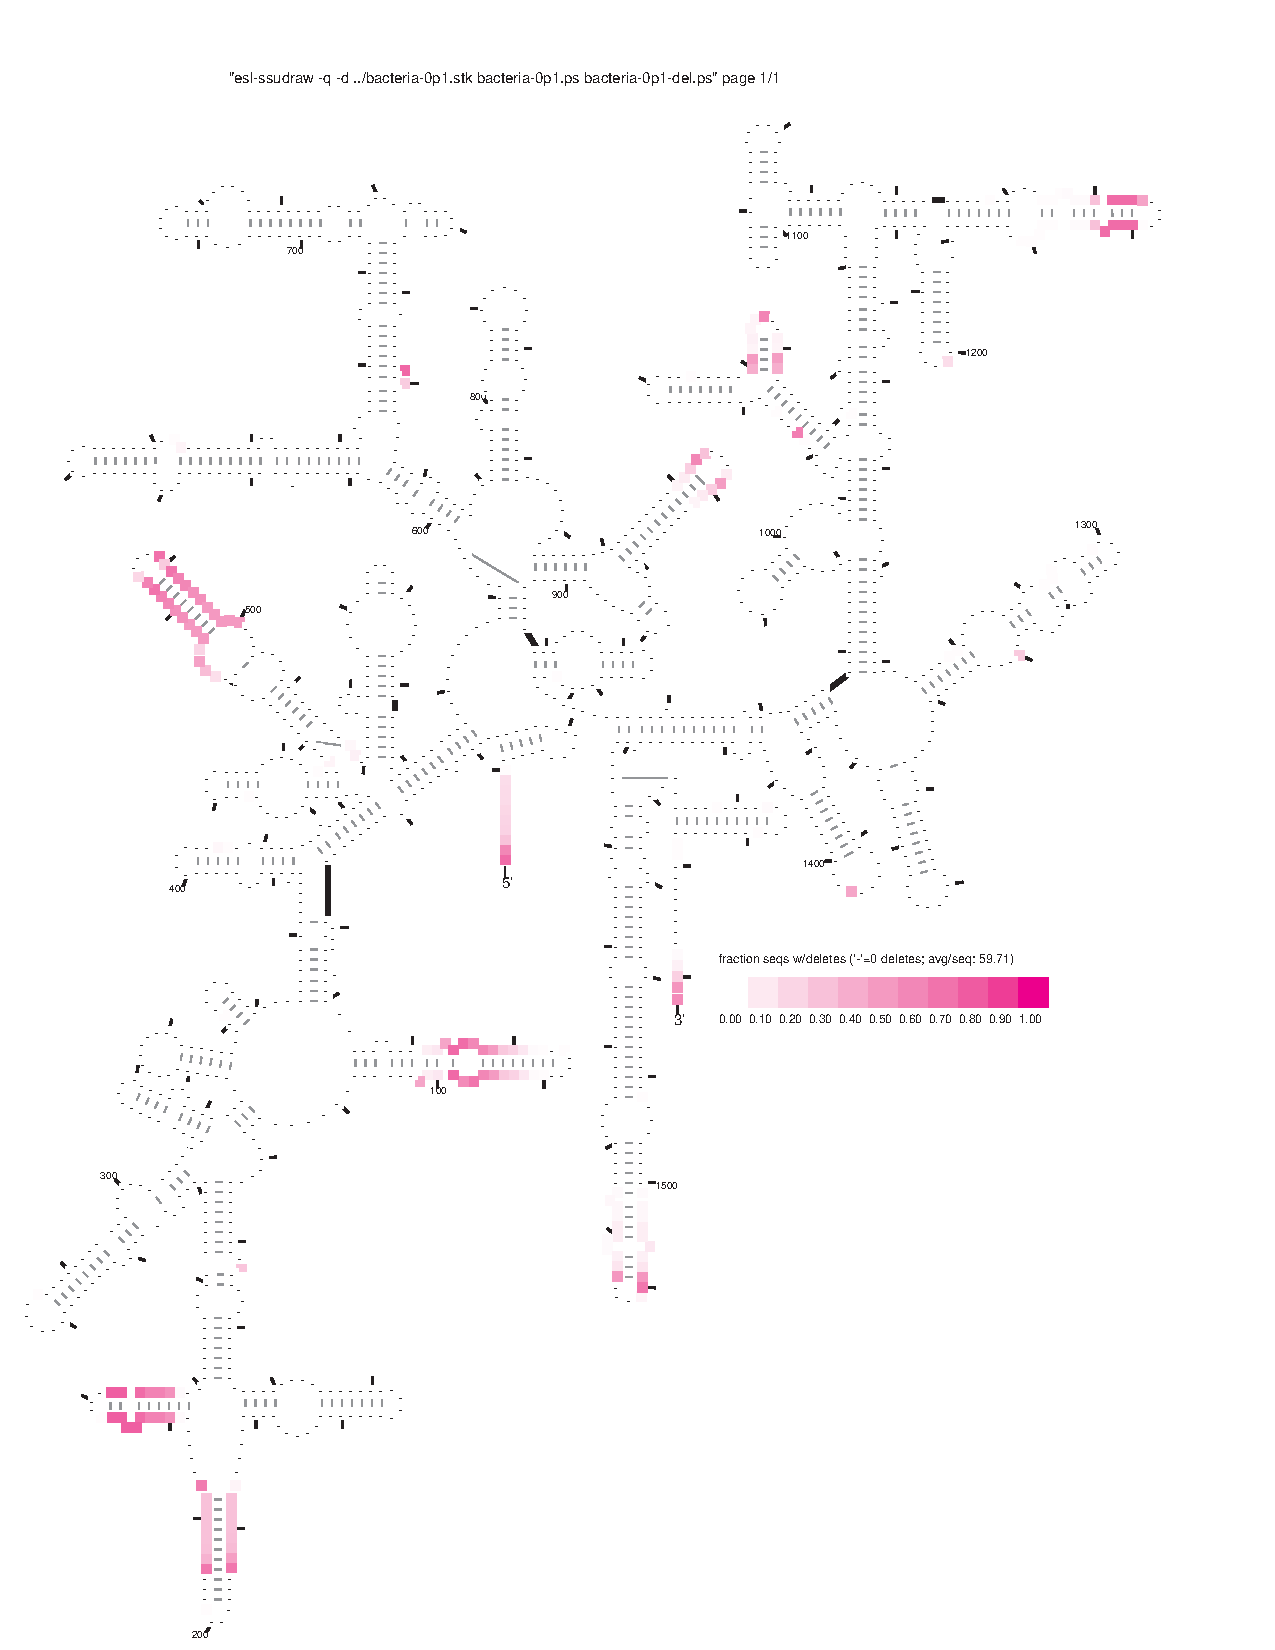
\includegraphics[height=8.5in]{../../seeds/ss-diagrams/bacteria-0p1-del}
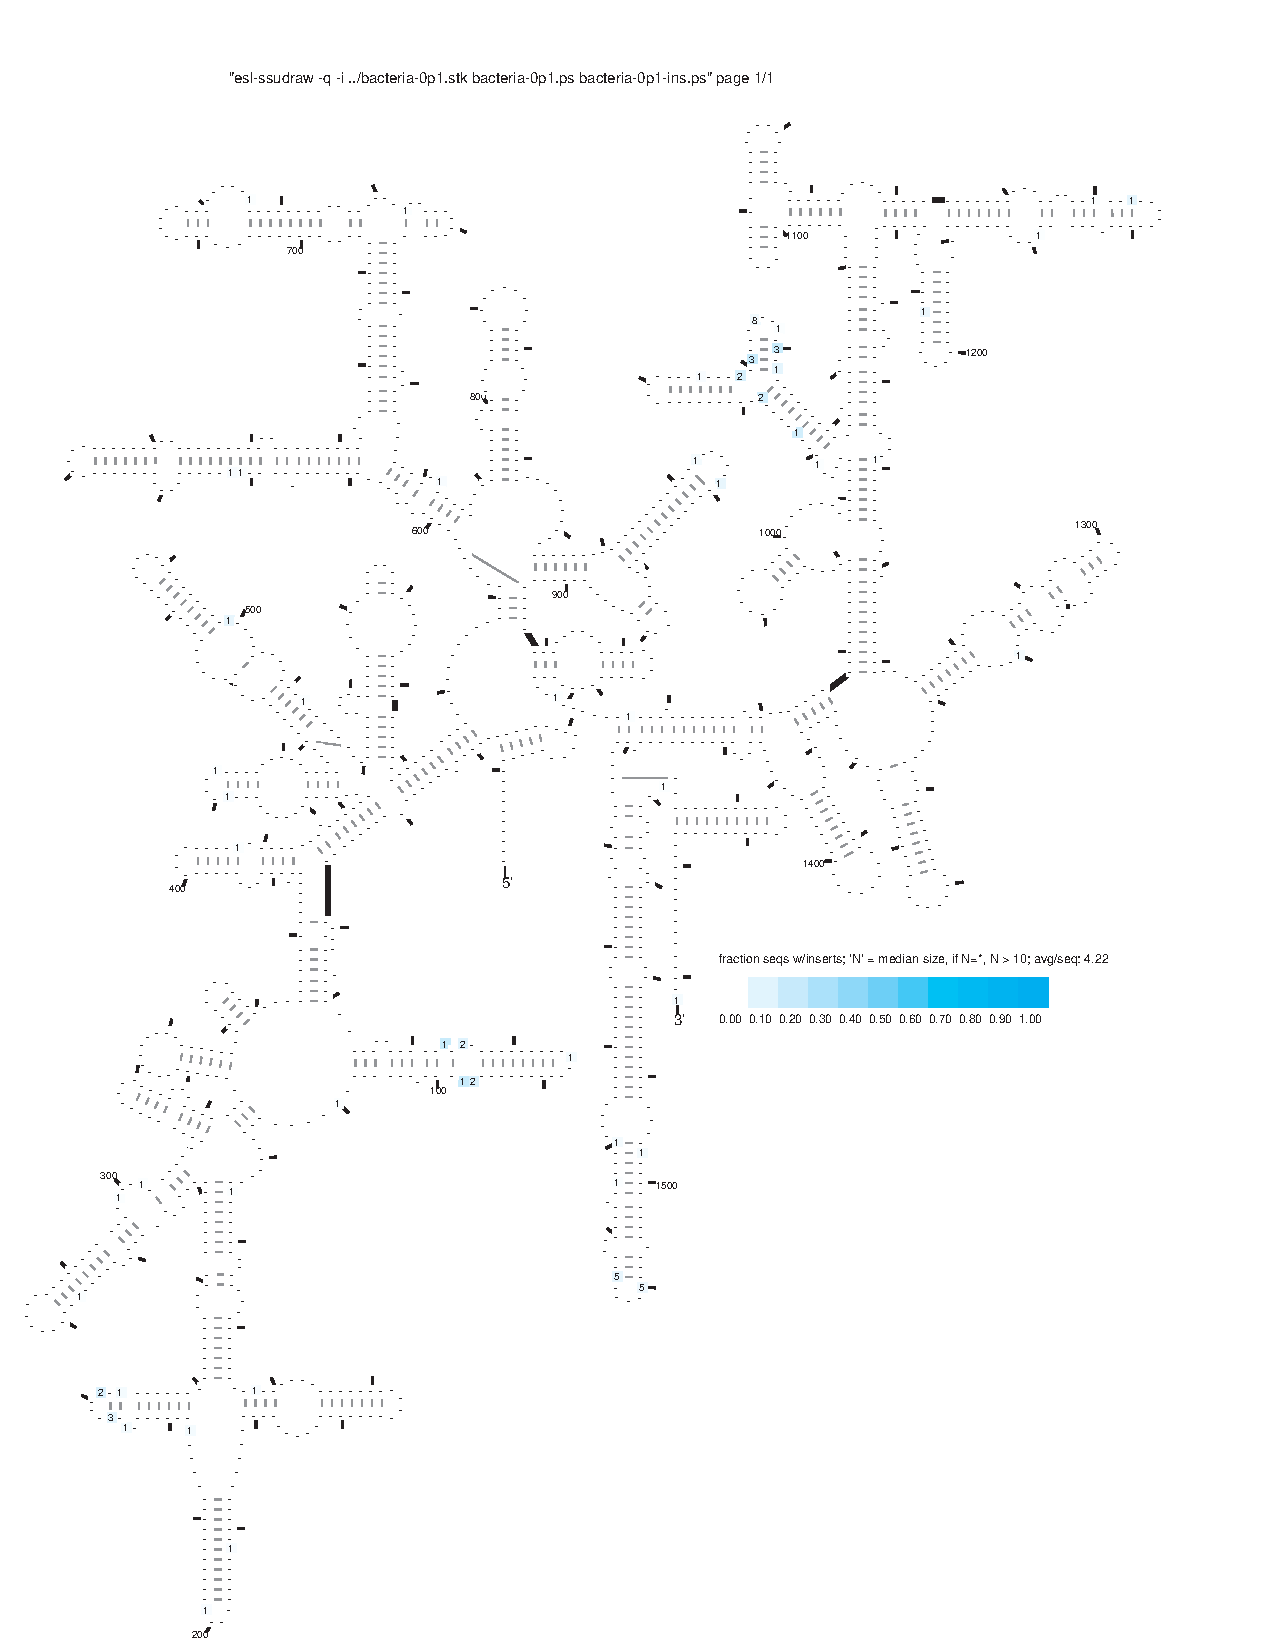
\includegraphics[height=8.5in]{../../seeds/ss-diagrams/bacteria-0p1-ins}

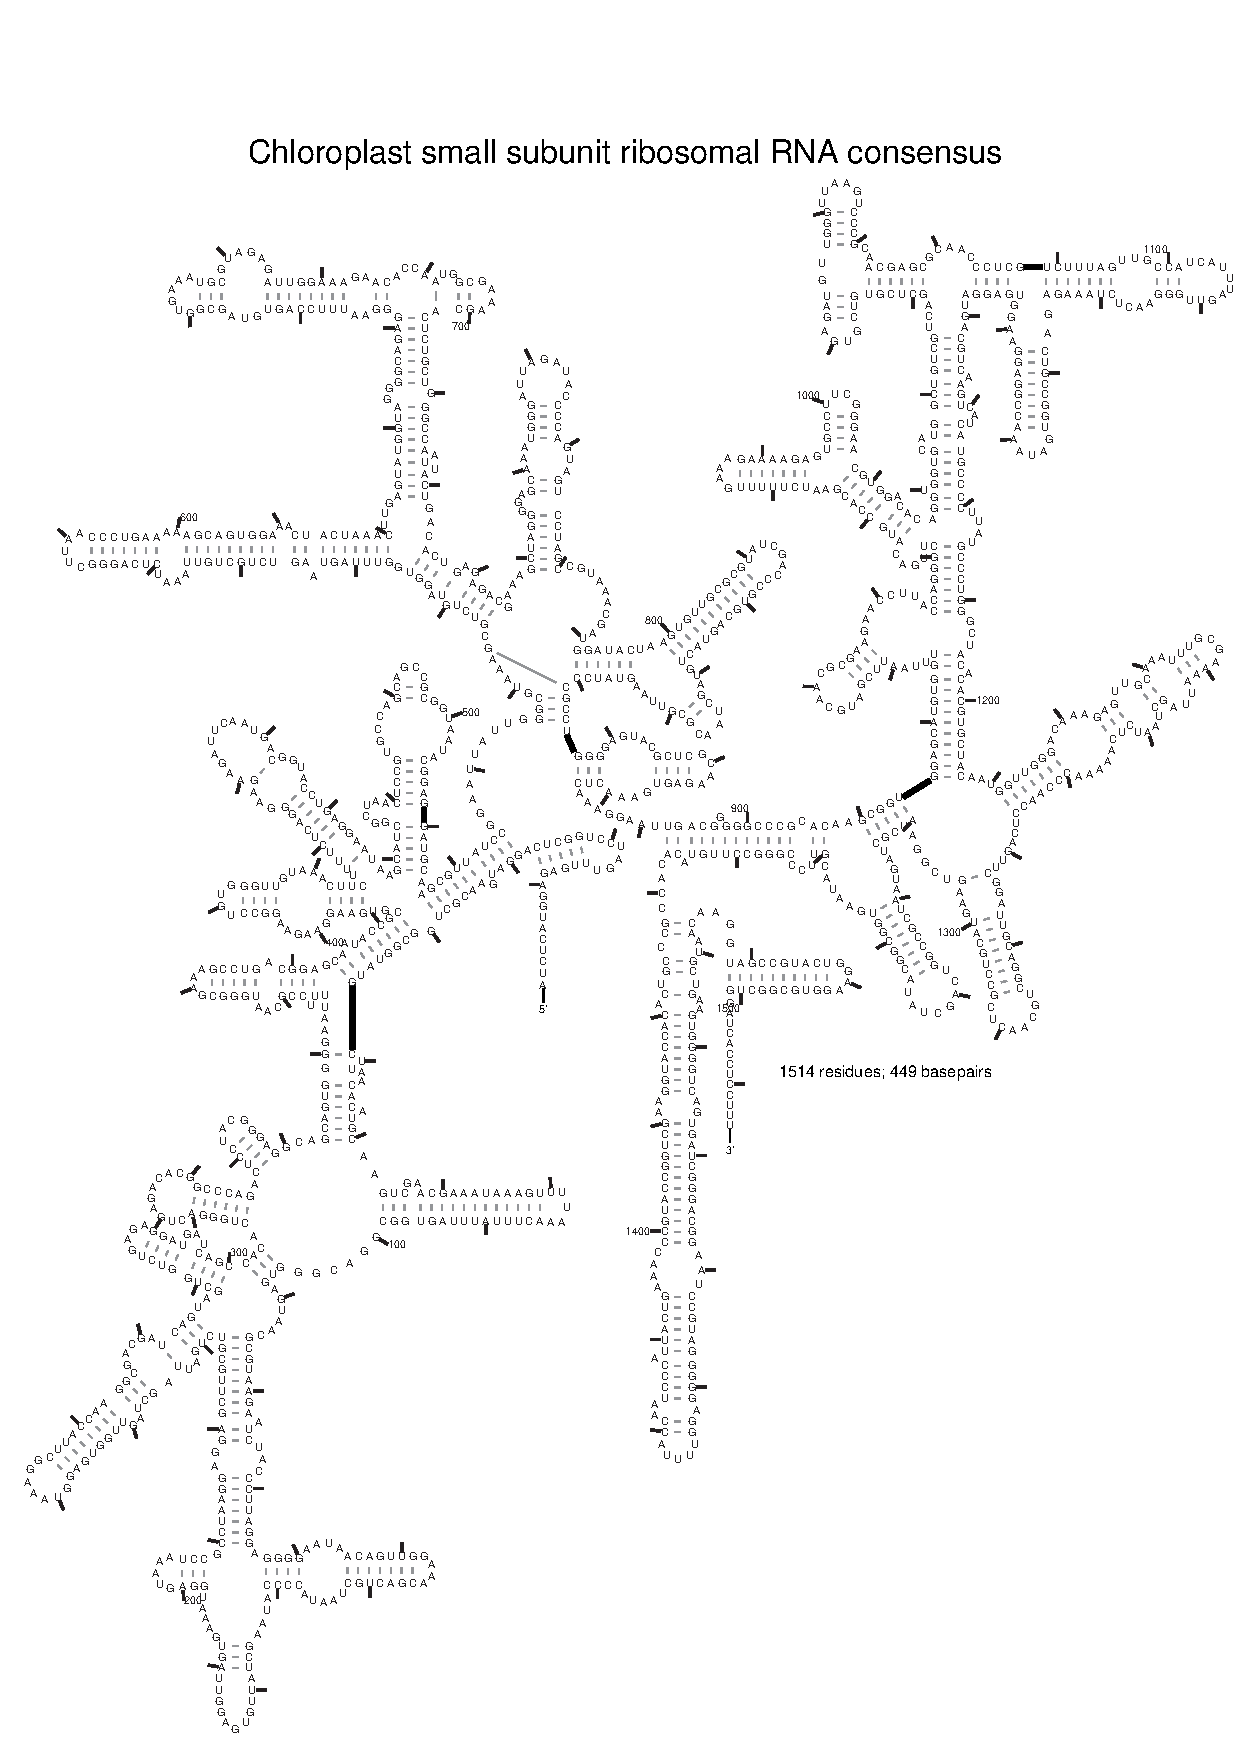
\includegraphics[height=8.5in]{../../seeds/ss-diagrams/chloroplast-0p1}
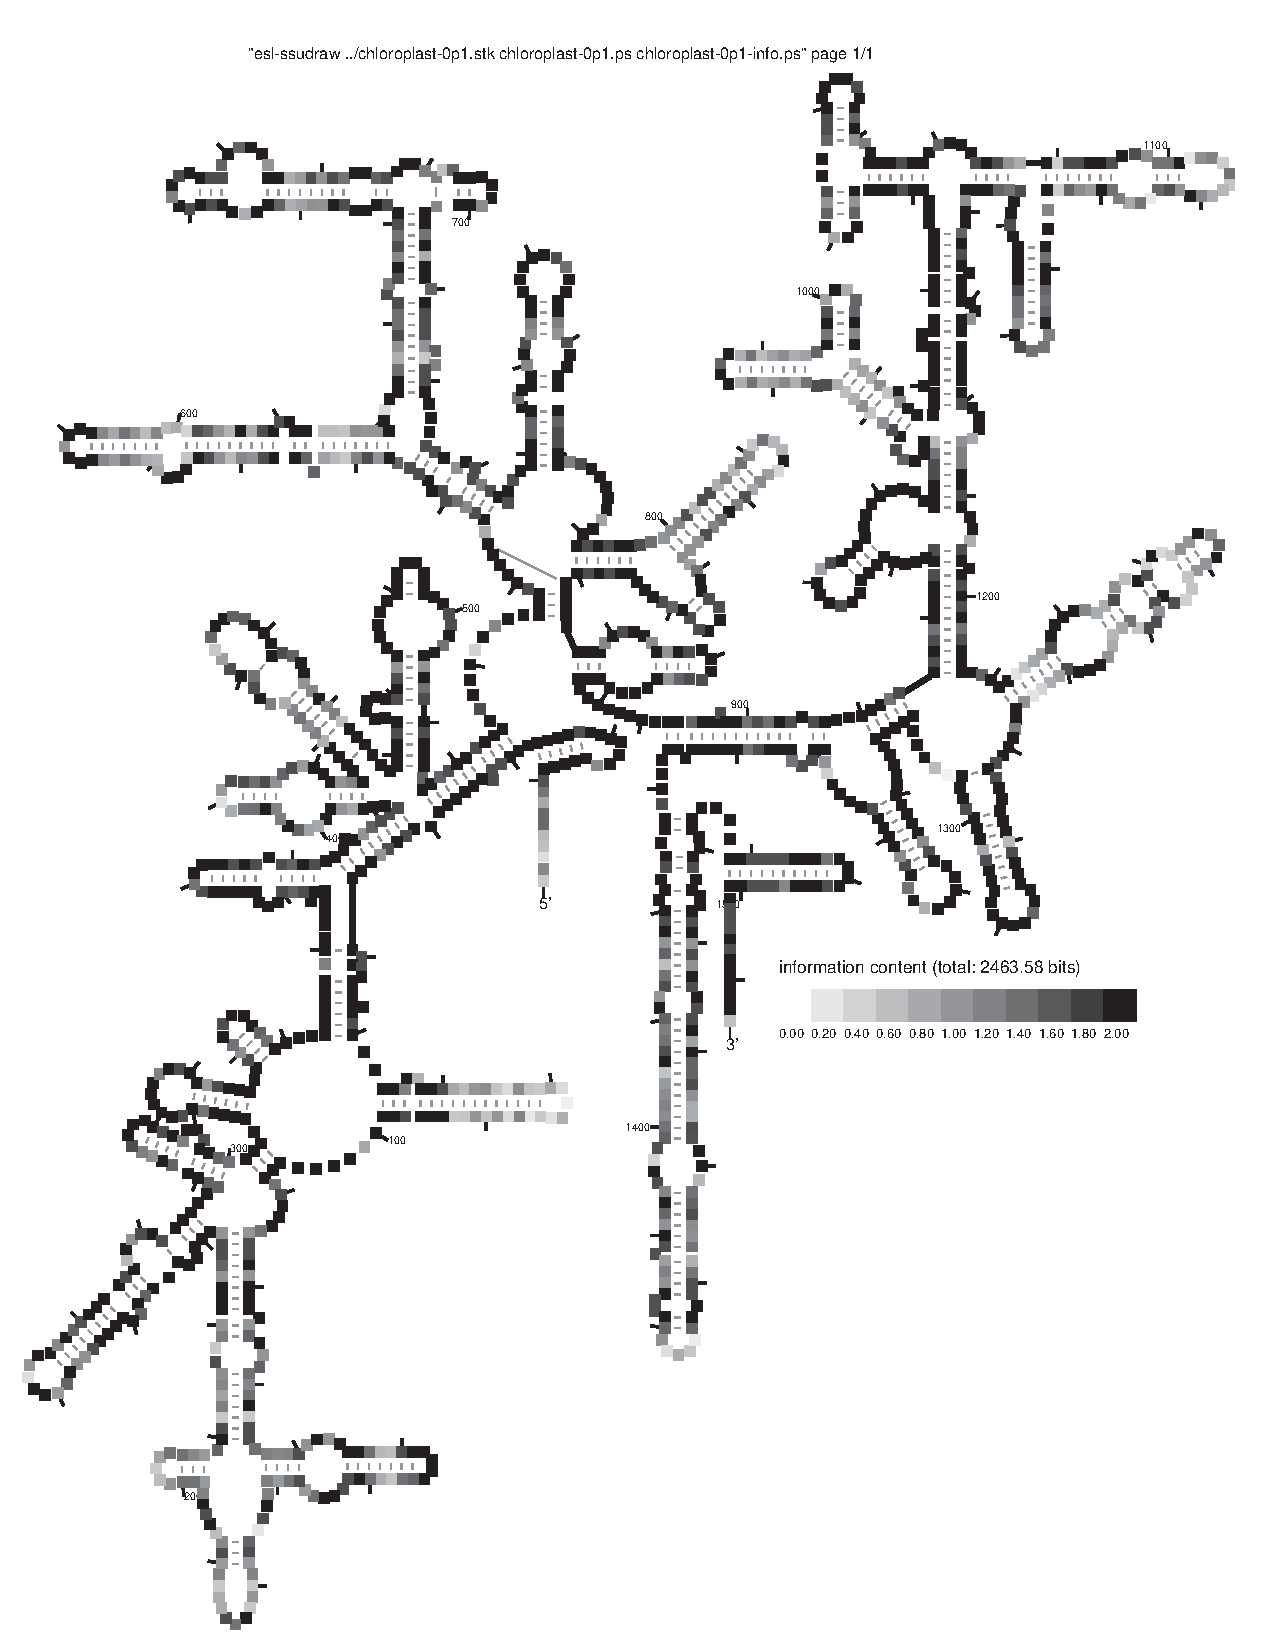
\includegraphics[height=8.5in]{../../seeds/ss-diagrams/chloroplast-0p1-info}
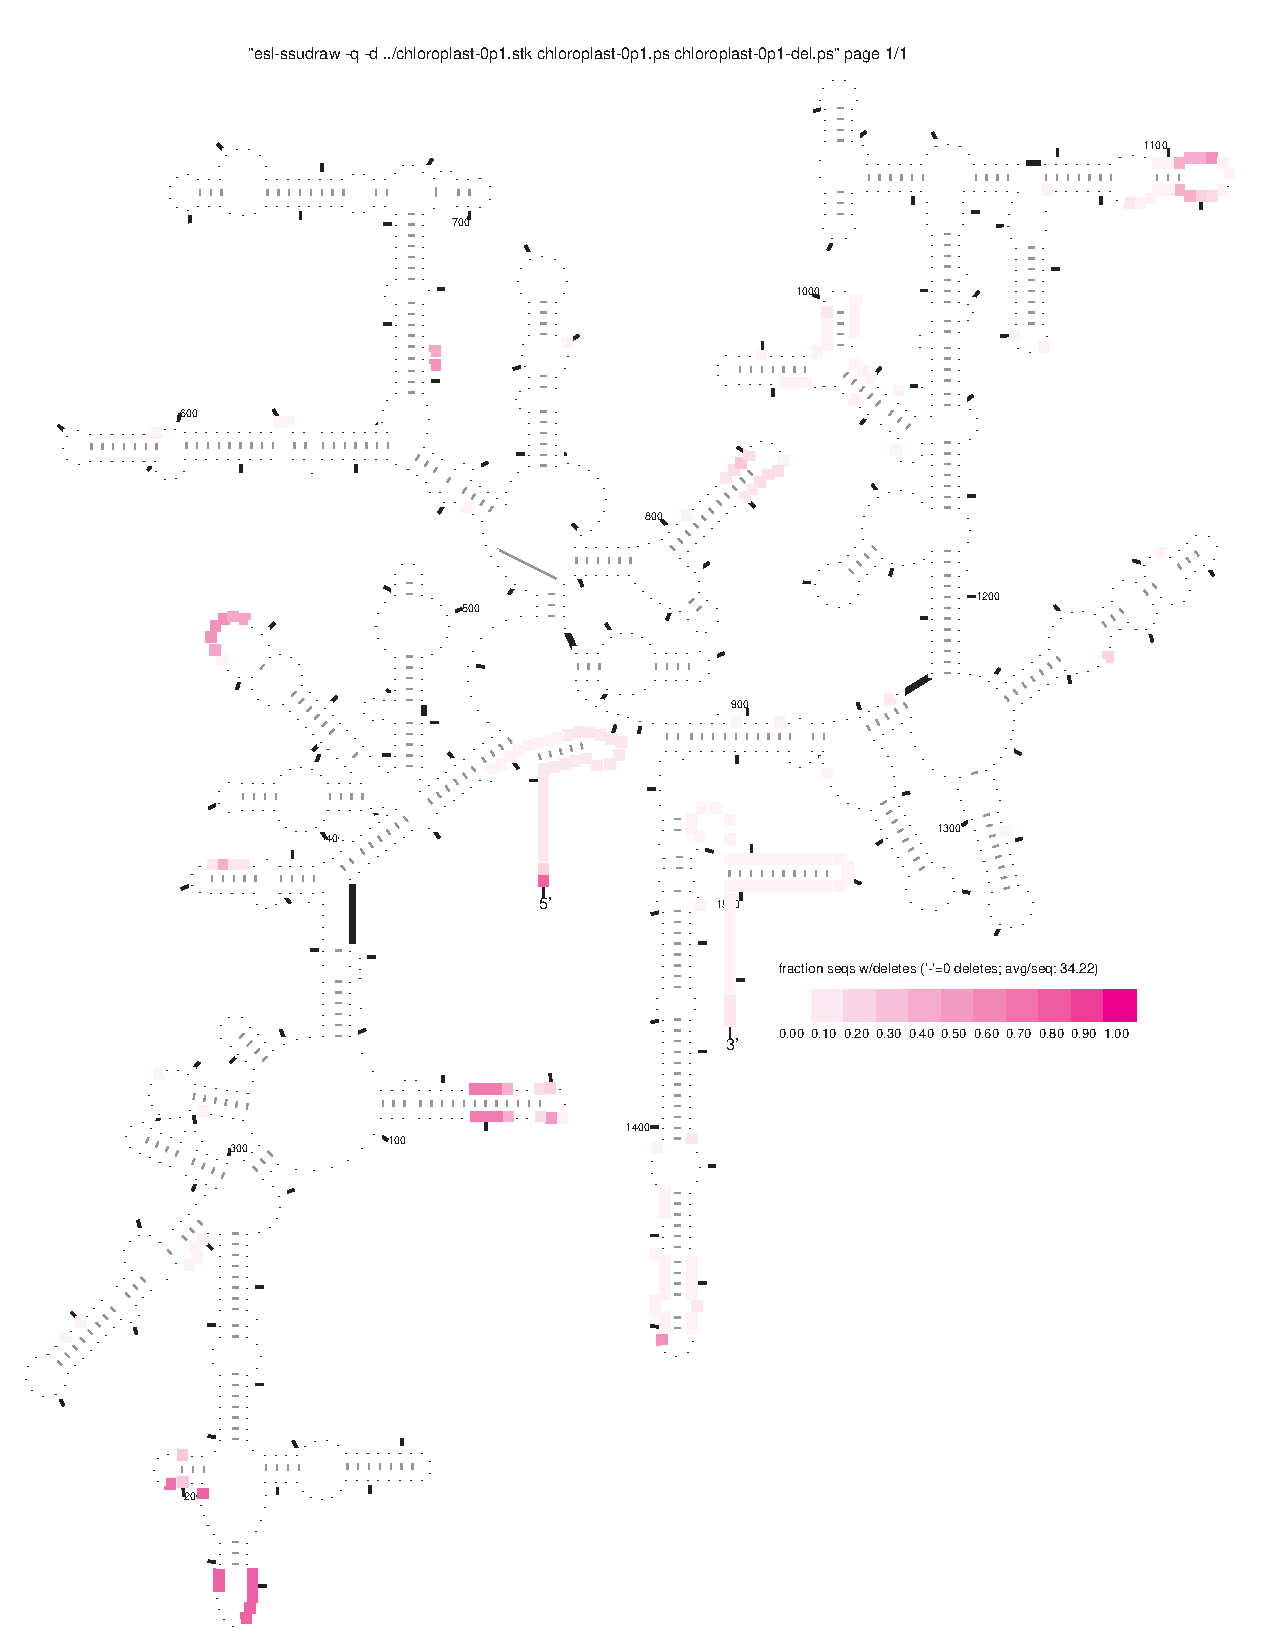
\includegraphics[height=8.5in]{../../seeds/ss-diagrams/chloroplast-0p1-del}
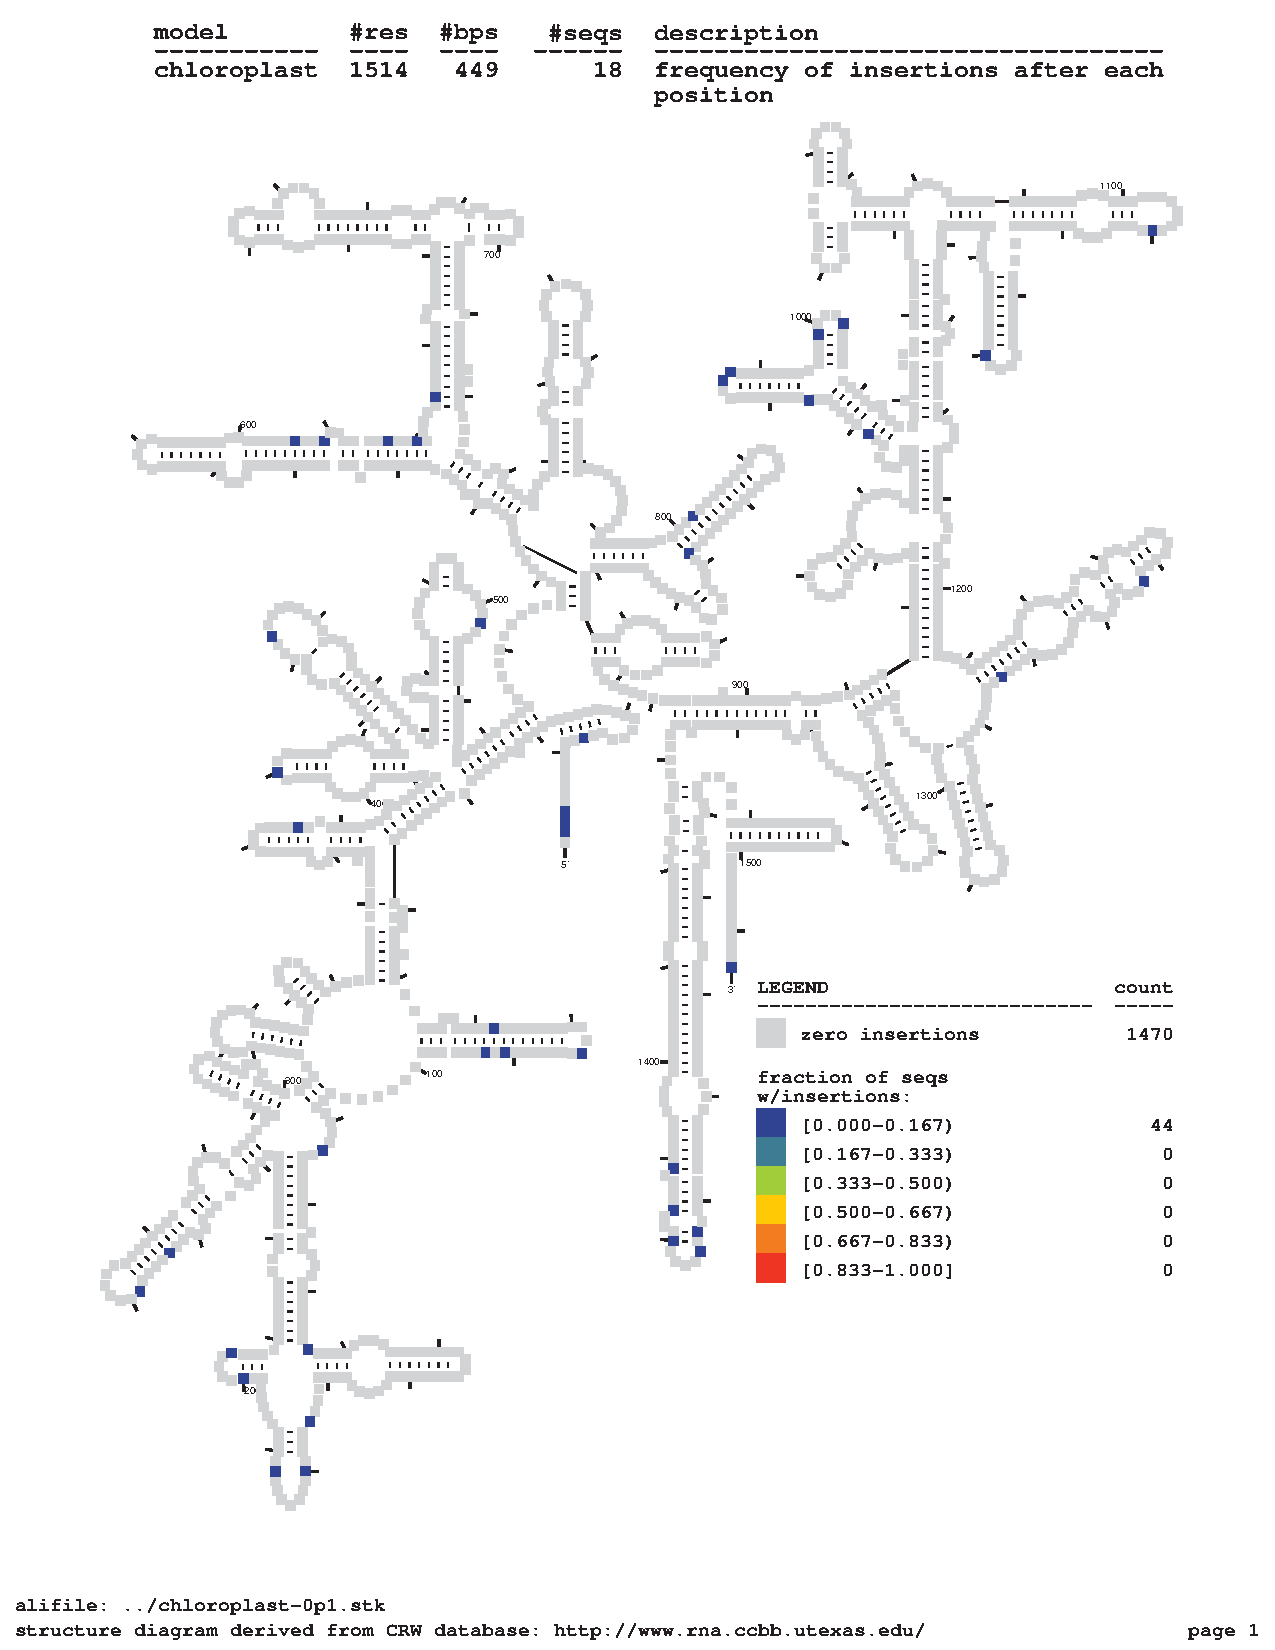
\includegraphics[height=8.5in]{../../seeds/ss-diagrams/chloroplast-0p1-ins}

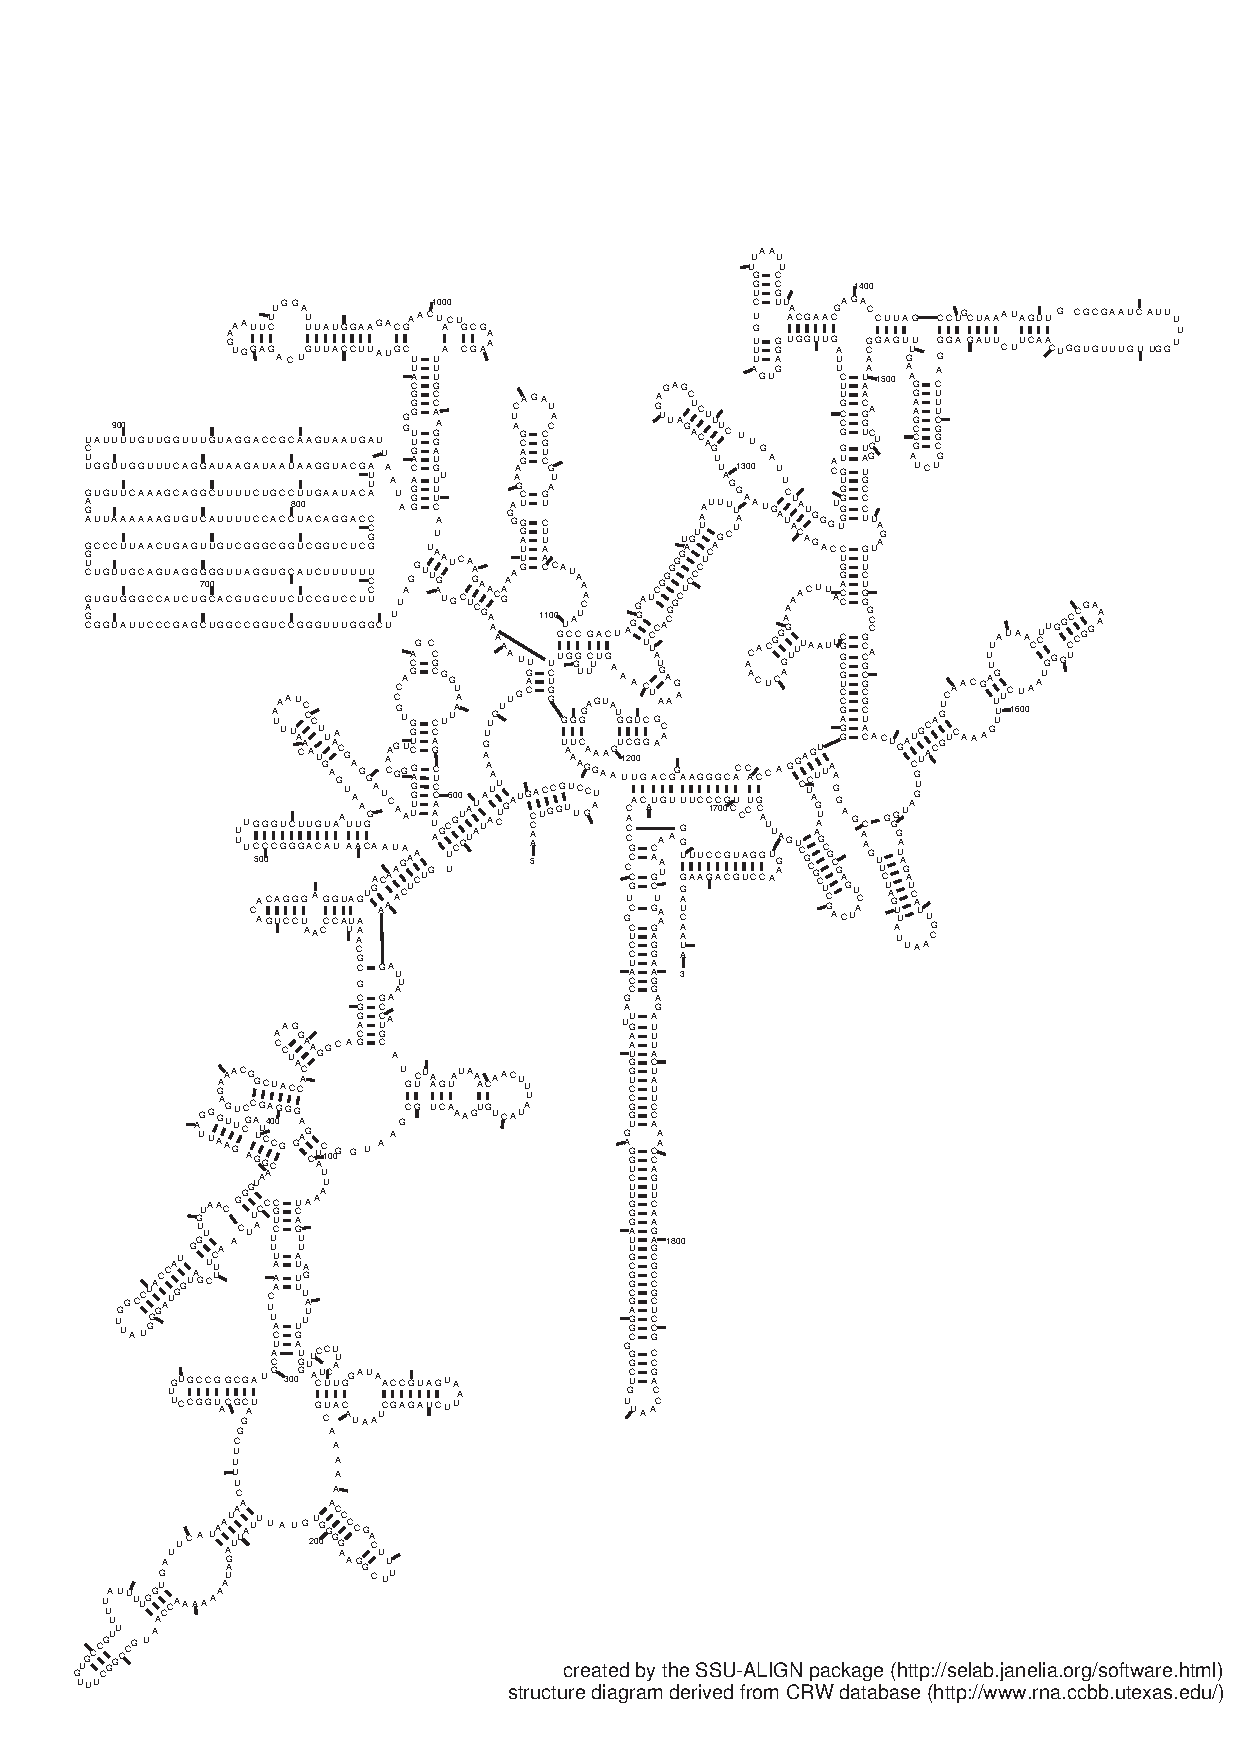
\includegraphics[height=8.5in]{../../seeds/ss-diagrams/eukarya-0p1}
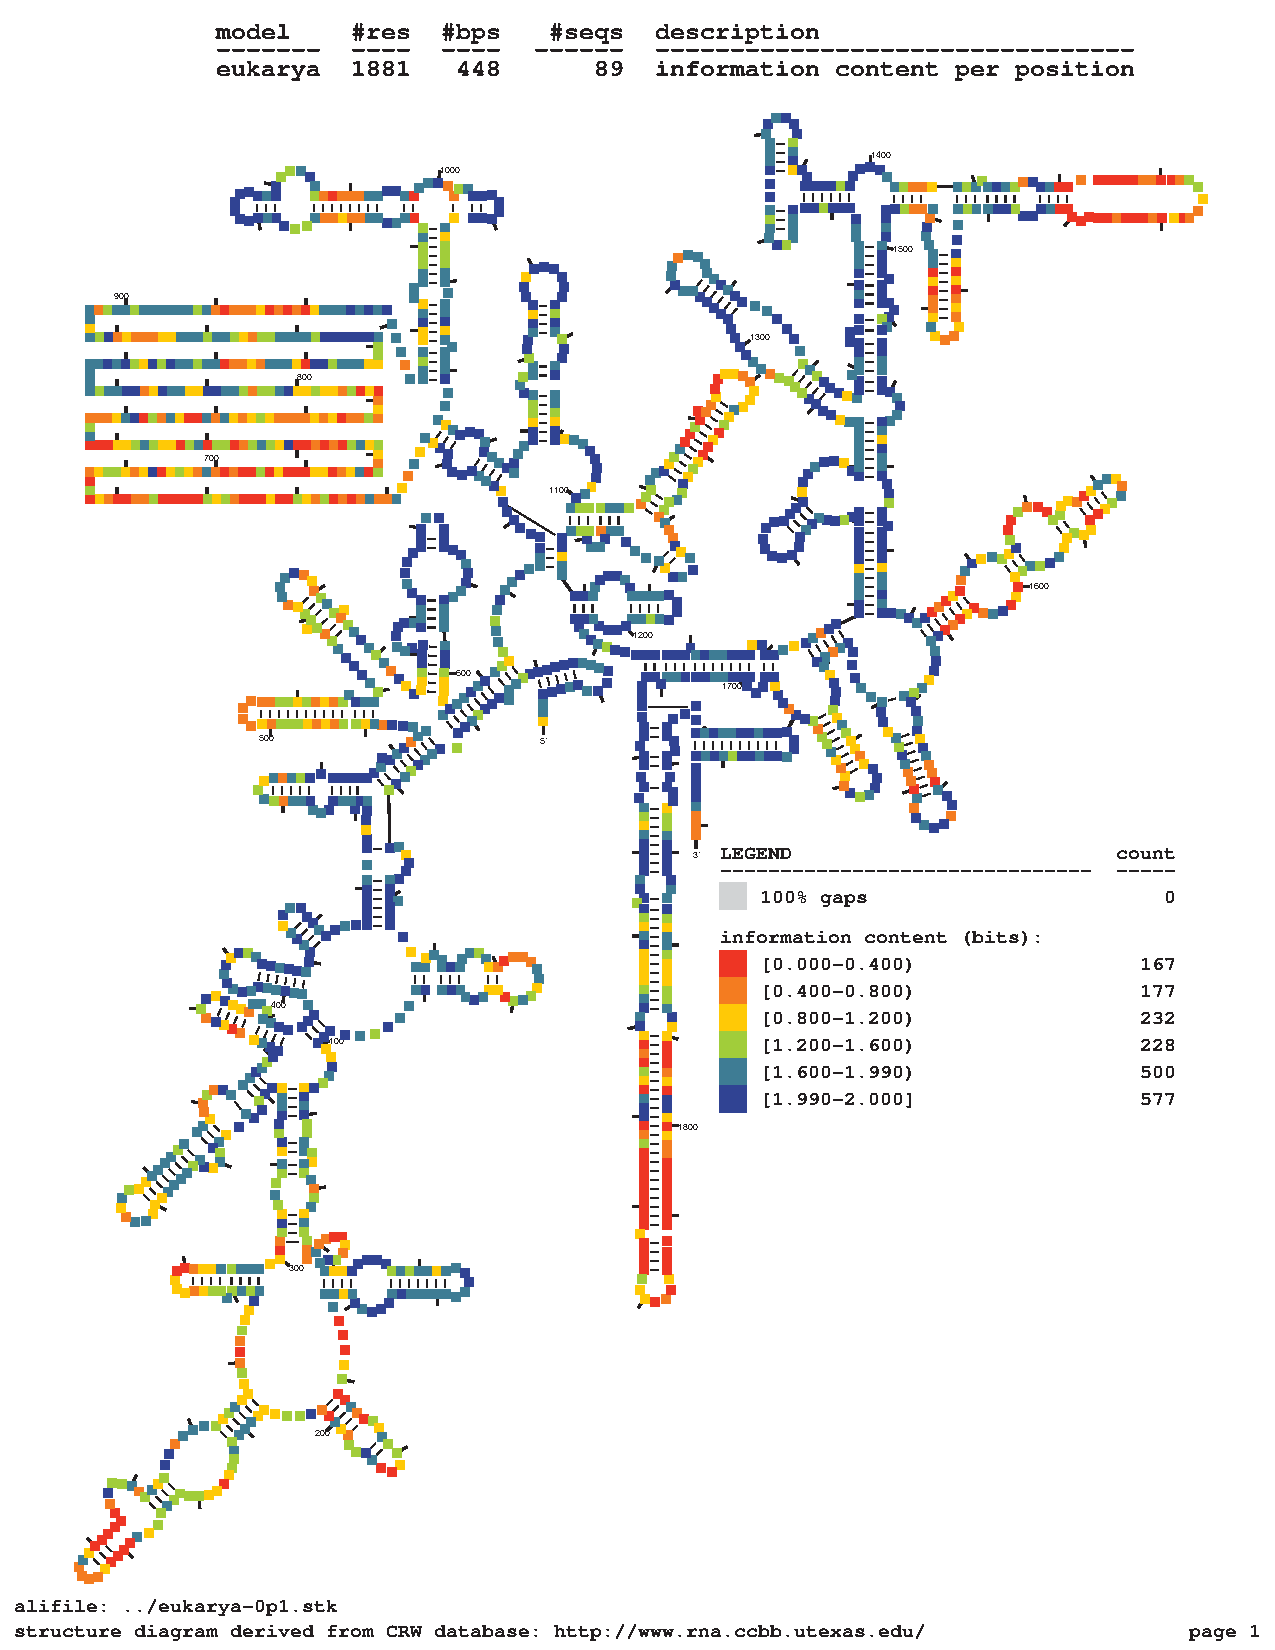
\includegraphics[height=8.5in]{../../seeds/ss-diagrams/eukarya-0p1-info}
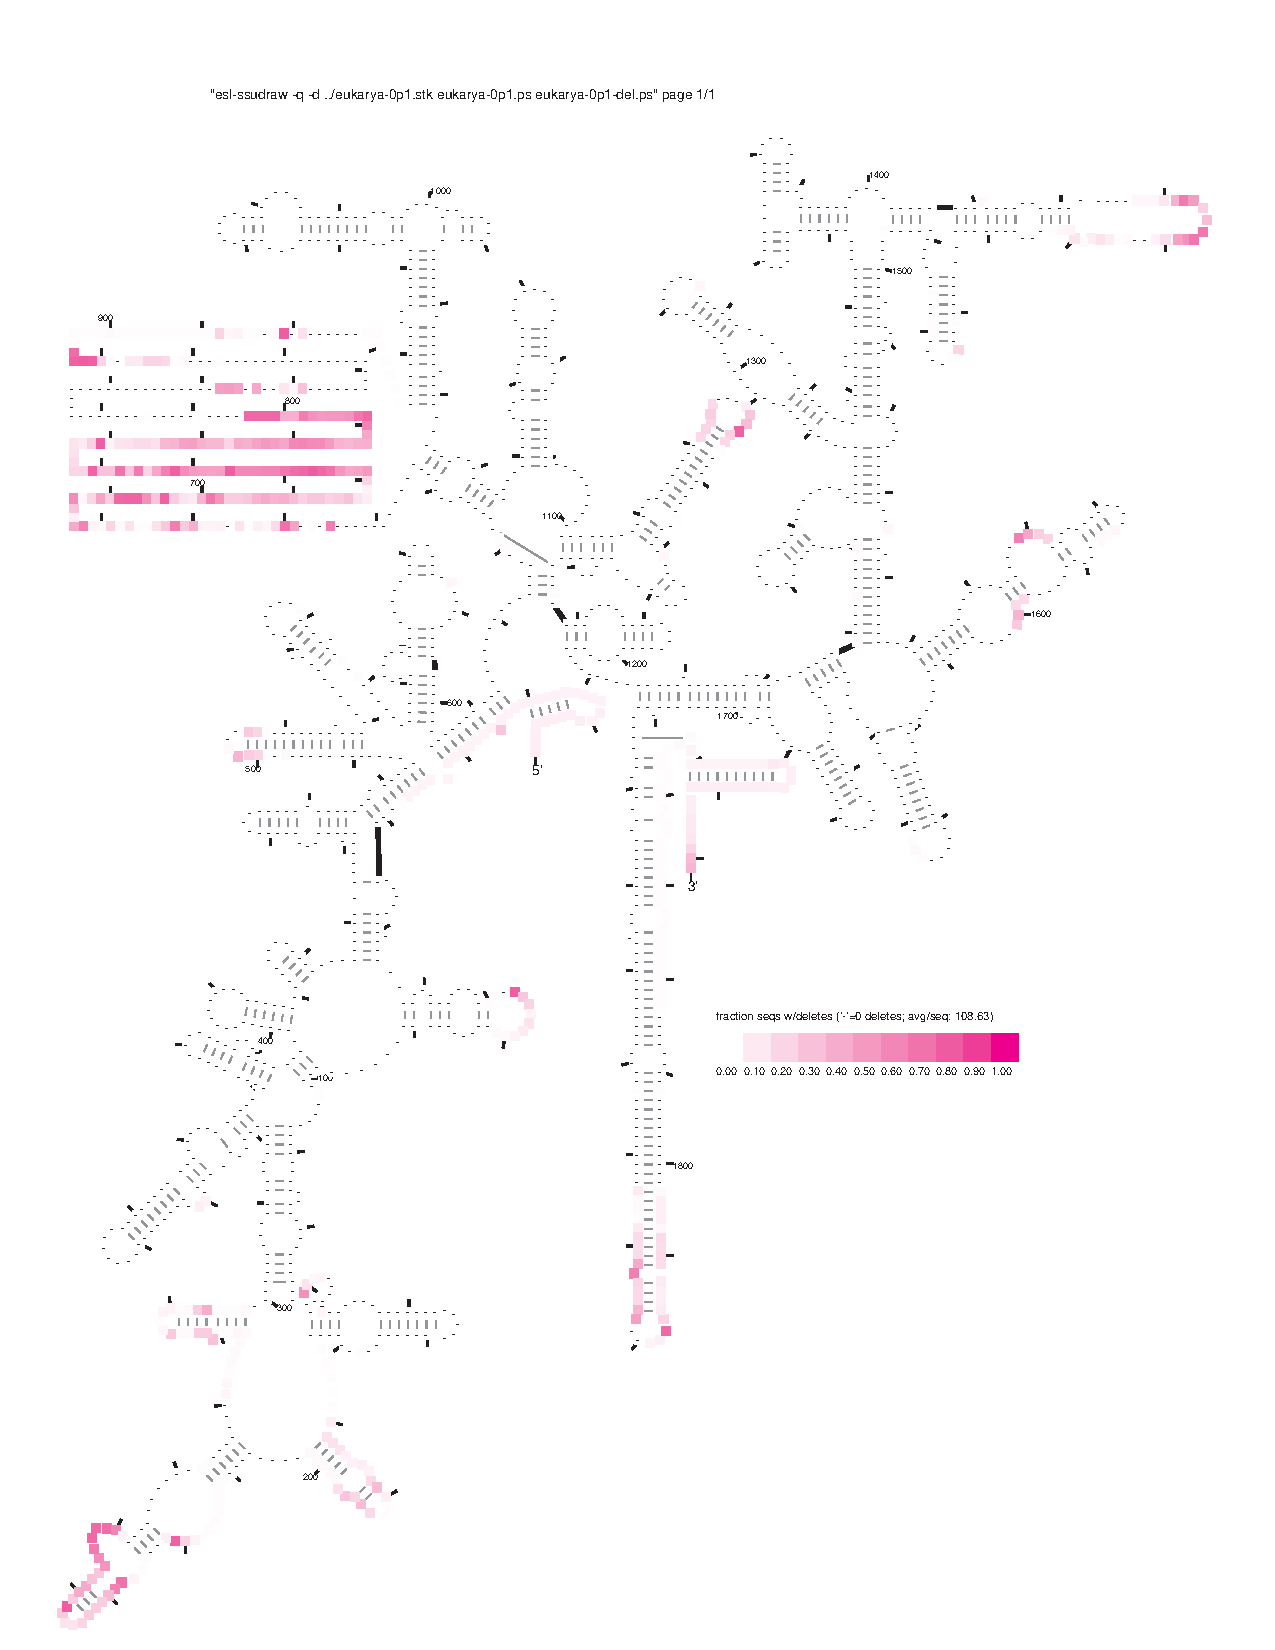
\includegraphics[height=8.5in]{../../seeds/ss-diagrams/eukarya-0p1-del}
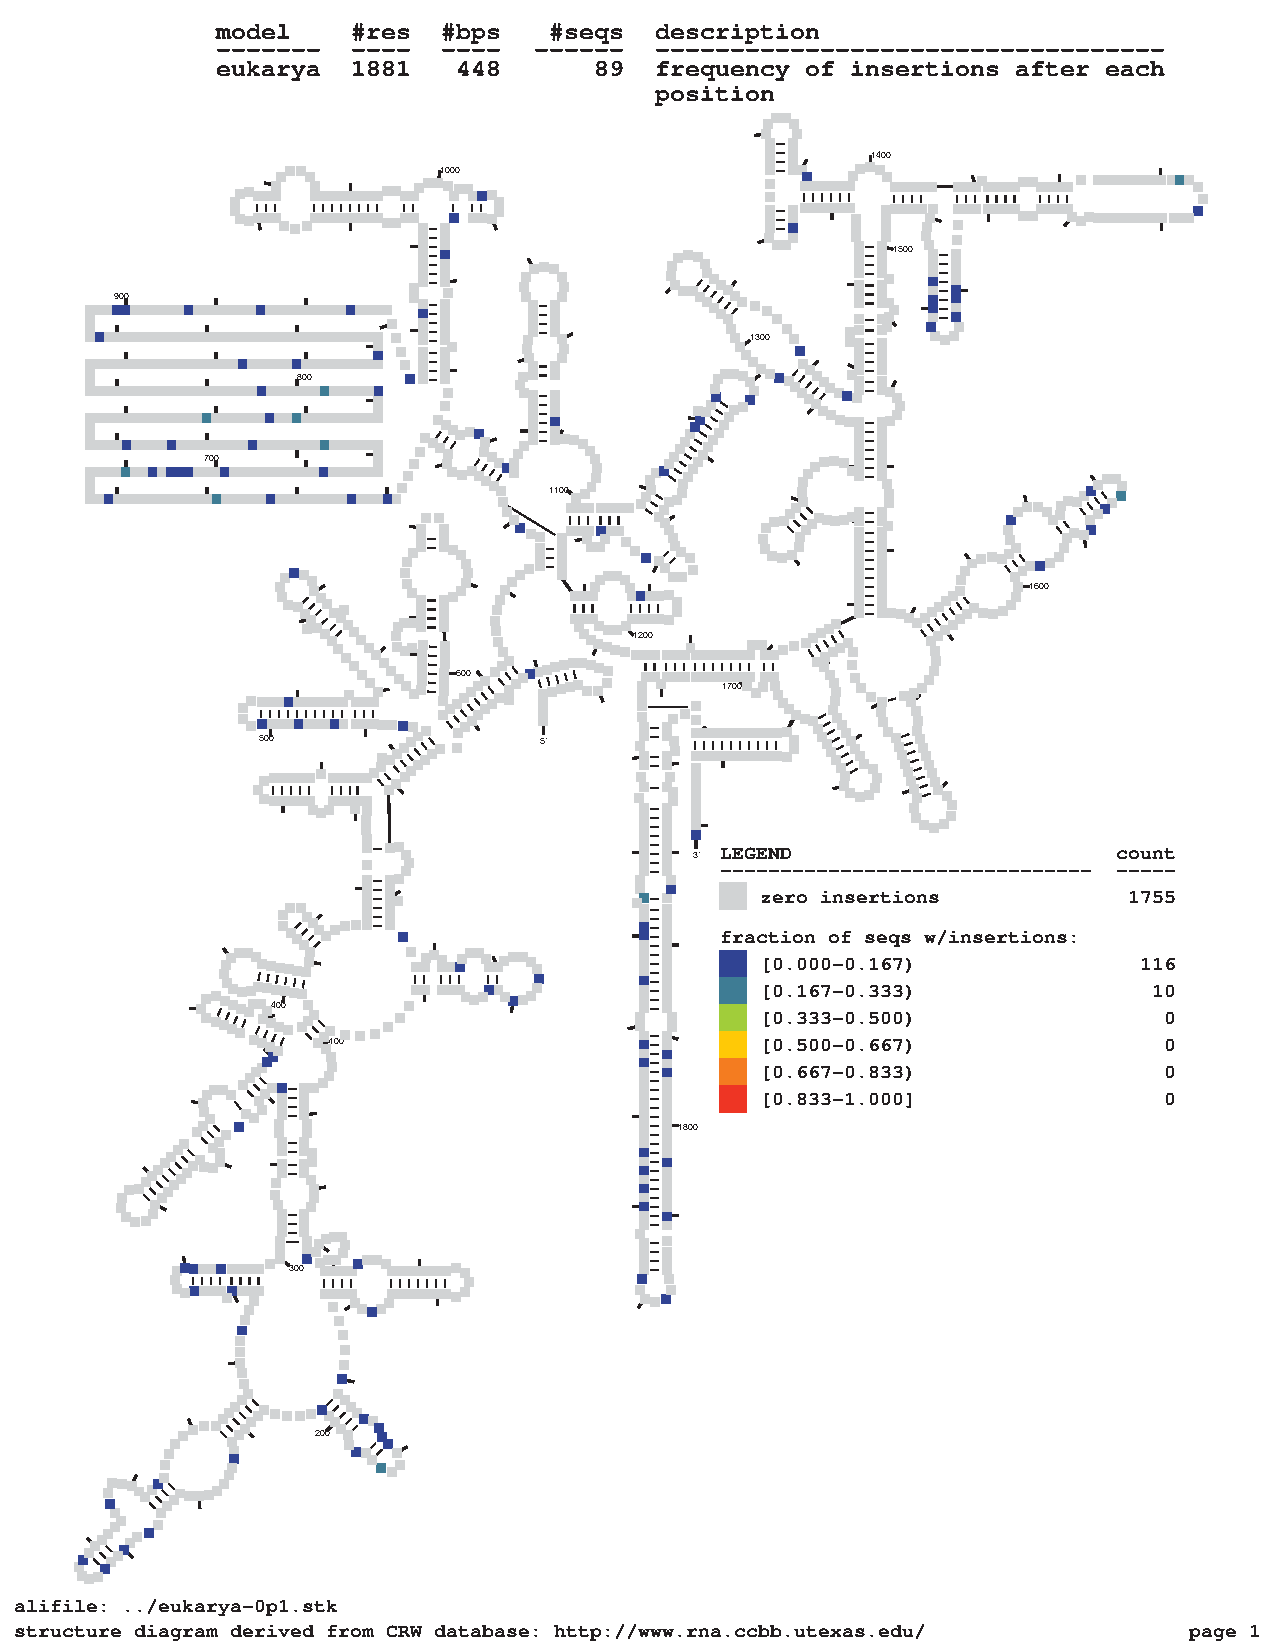
\includegraphics[height=8.5in]{../../seeds/ss-diagrams/eukarya-0p1-ins}

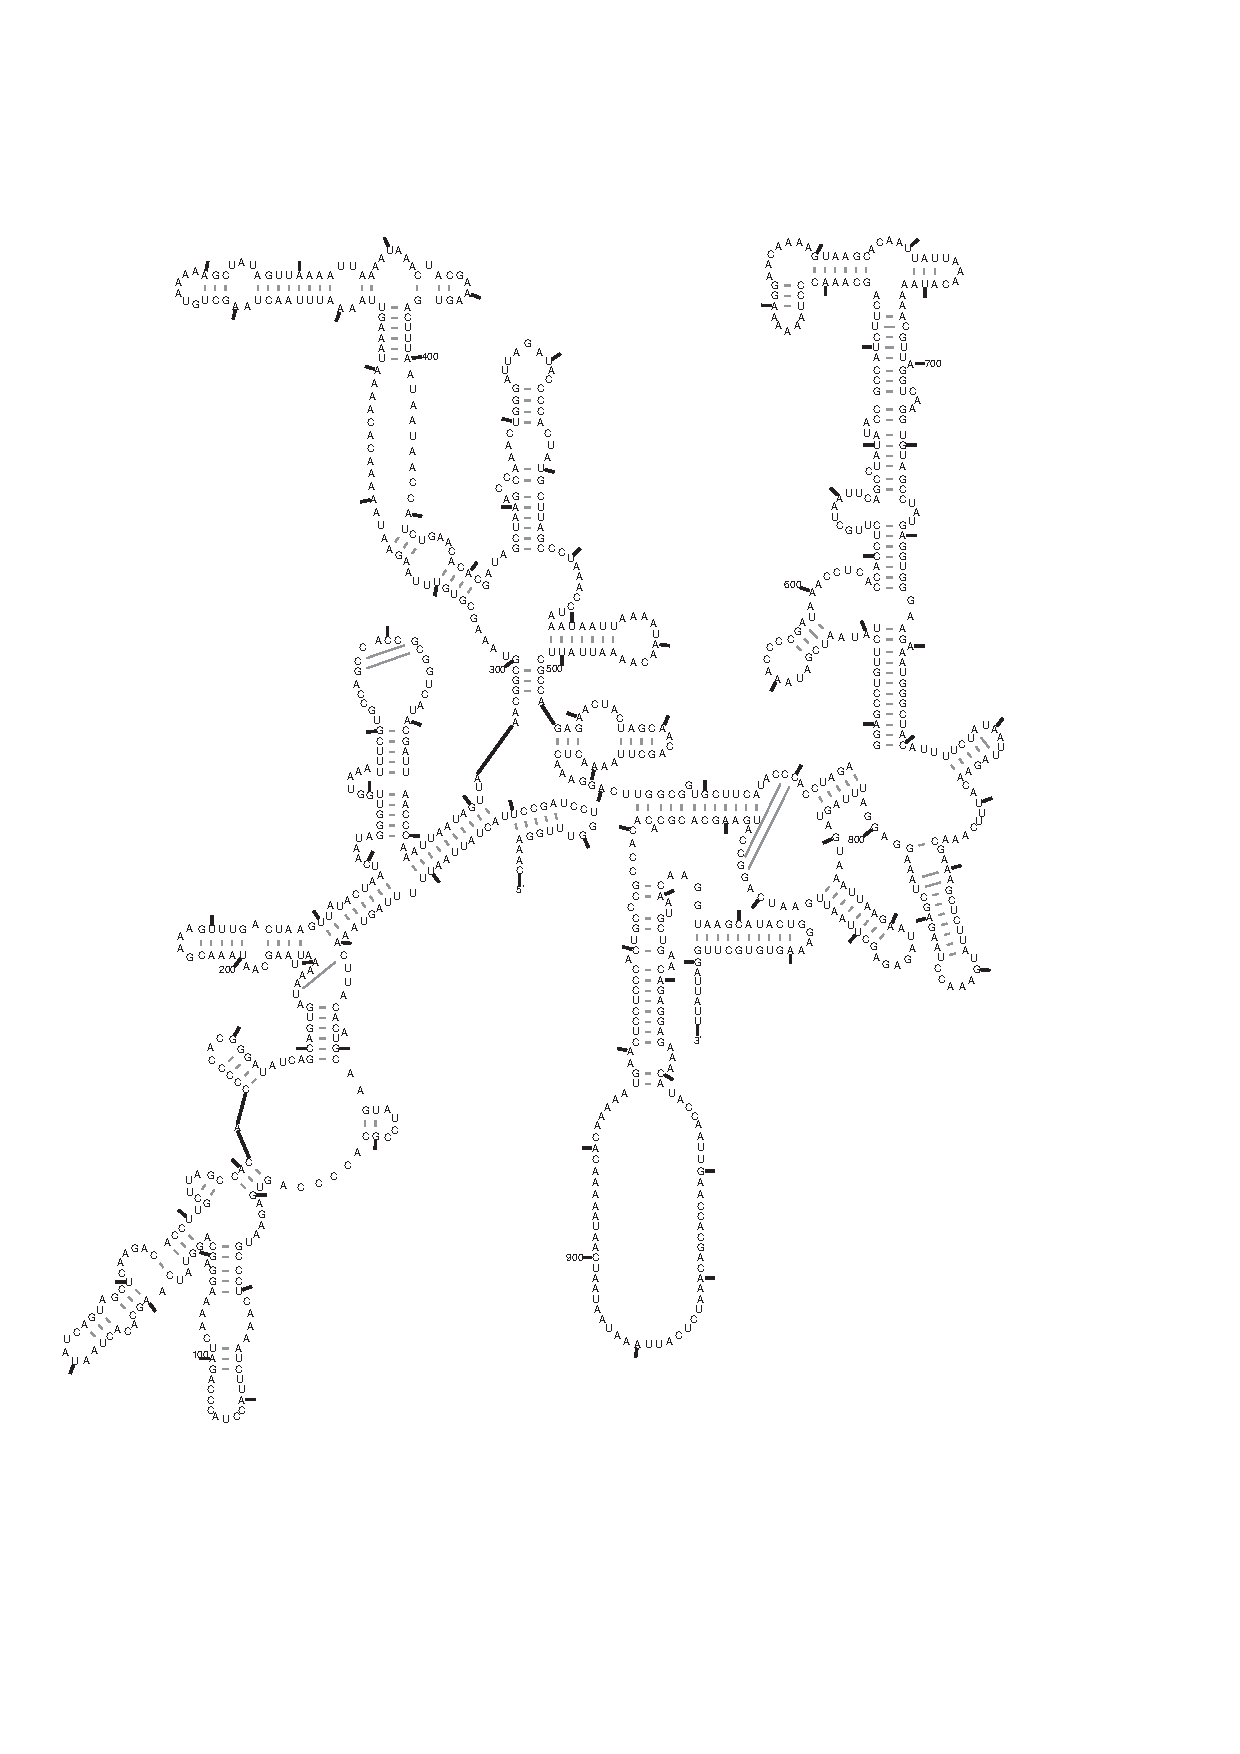
\includegraphics[height=8.5in]{../../seeds/ss-diagrams/metamito-0p1}
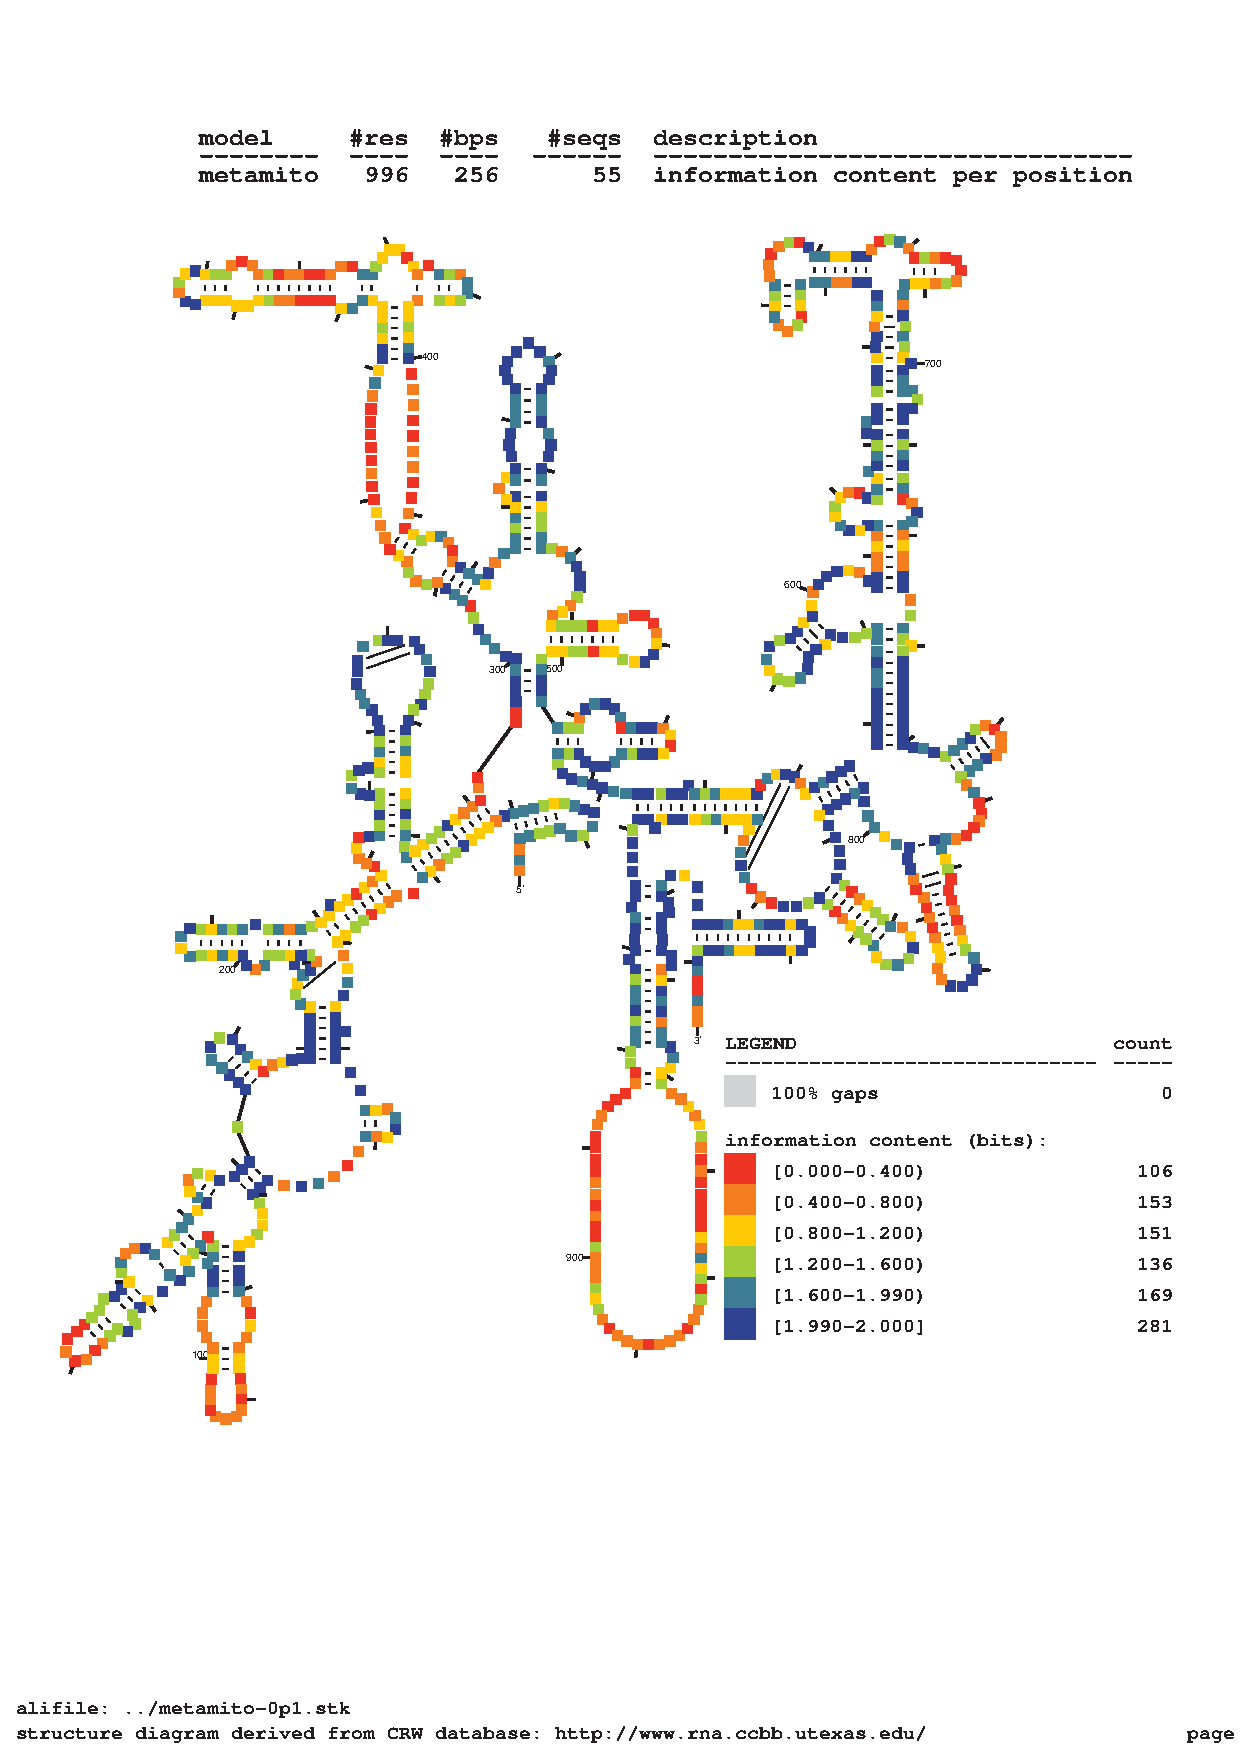
\includegraphics[height=8.5in]{../../seeds/ss-diagrams/metamito-0p1-info}
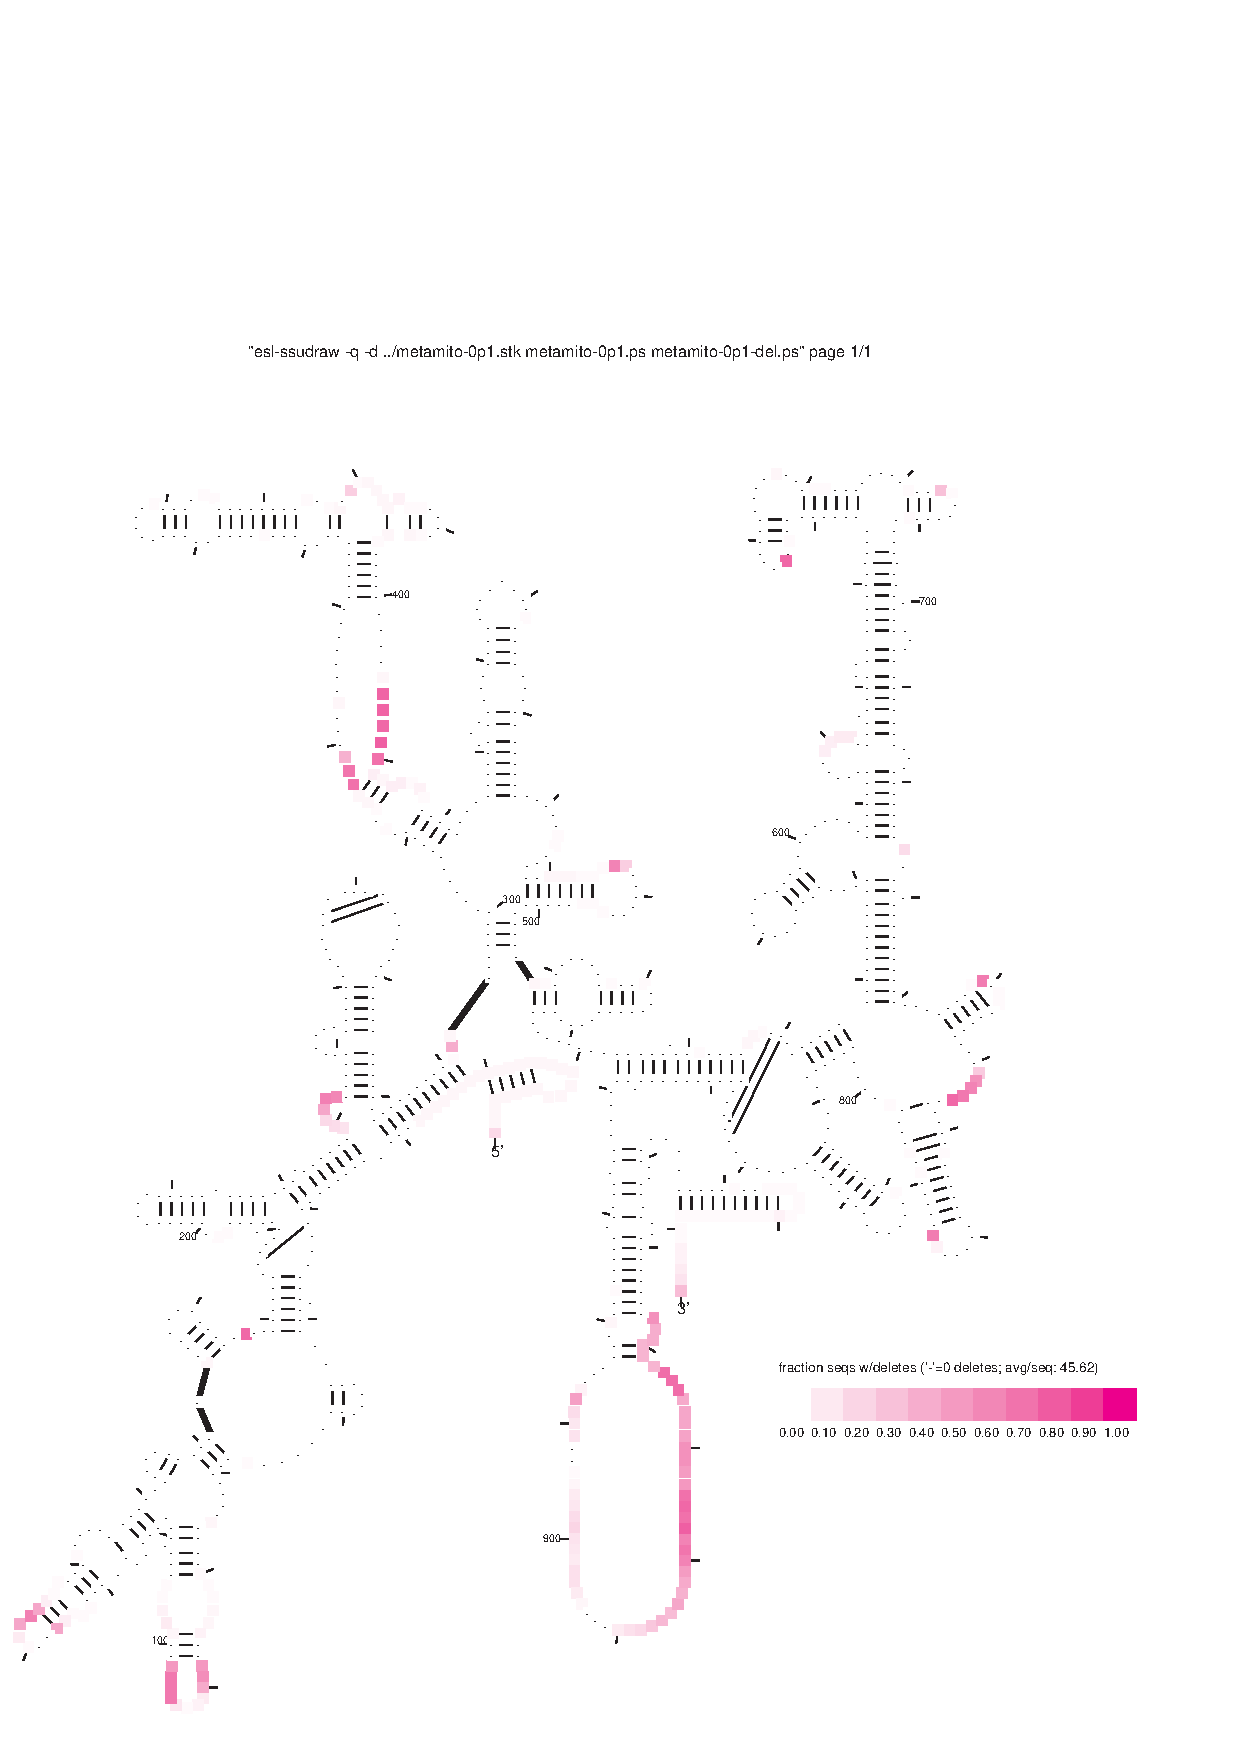
\includegraphics[height=8.5in]{../../seeds/ss-diagrams/metamito-0p1-del}
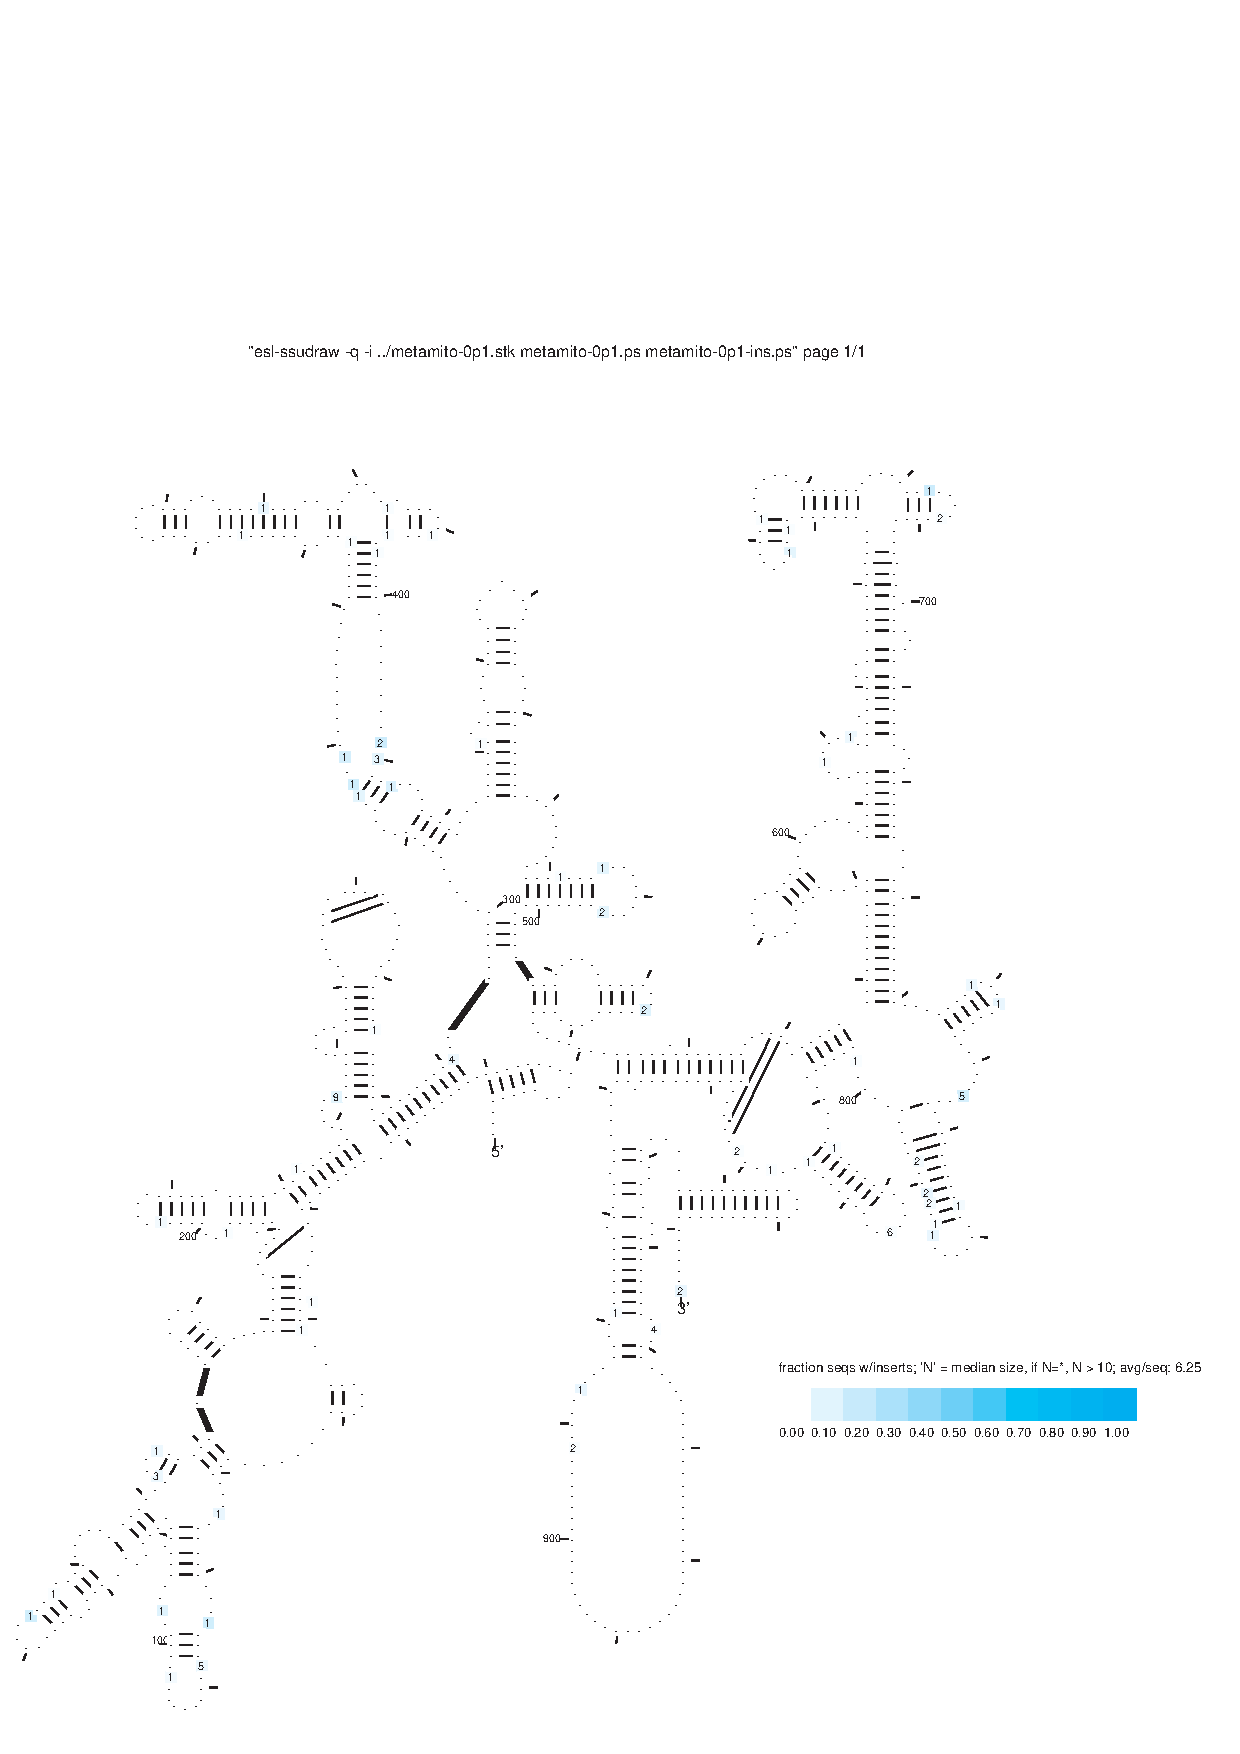
\includegraphics[height=8.5in]{../../seeds/ss-diagrams/metamito-0p1-ins}
\end{comment}

\subsection{Sequence diversity in the seed alignments}

TO DO: LIST HOW MANY SEQUENCES IN EACH PHYLA (or some other classification level)









\section{How SSU-ALIGN's default alignment masks were determined}
\label{sec:masks}

This section describes how the default alignment masks used by
\software{ssu-align} were determined. There are three default masks,
one for each of the three default models: archaea, bacteria and
eukarya.

The masks were determined based on large datasets
of SSU sequences. Specifically, subsets of all the SSU sequences in
the  January 24, 2010 release of the \software{greengenes} database 
\cite{DeSantis06} and the \emph{Ref} set of SSU rRNA sequences from
release 100 of the \software{silva} database
\cite{Pruesse07} were used. Table~\ref{tbl:ggsil} includes statistics
on these alignments. 

The first step towards determining the masks was to run
\prog{ssu-align} with the \prog{--no-align} option on the combined
\software{Silva} \emph{Ref} and \software{greengenes} unaligned
datasets, in FASTA format. If the combined dataset is in the file
\prog{ggsil.fa}, this could be reproduced using the command:

\user{ssu-align --no-align ggsil.fa ggsil}

From this, three new FASTA files are created in the new directory
\prog{ggsil/}: \prog{ggsil.archaea.fa}, \\ \prog{ggsil.bacteria.fa},
and \prog{ggsil.eukarya.fa}, 
the predicted set of archaeal, bacterial and eukaryotic
SSU sequences (possibly with some of the original
\software{greengenes} or \software{silva} sequence trimmed away from
the ends). 

Next, I used Robert Edgar's fast \software{uclust} tool (version 1.0.50) to
remove redundancy from each of these sets of sequences. Specifically, for
archaea, I executed the following three \prog{uclust} commands:

\user{uclust1.0.50\_linuxi86\_64 --sort ggsil.archaea.fa --output ggsil.sorted.archaea.fa}

\user{uclust1.0.50\_linuxi86\_64 --input ggsil.sorted.archaea.fa --uc \\  ggsil.f97.archaea.uc --id 0.97}

\user{uclust1.0.50\_linuxi86\_64 --input ggsil.sorted.archaea.fa --uc2fasta \\ ggsil.f97.archaea.uc --types S --output ggsil.f97.archaea.fa}

The final output file is \prog{ggsil.f97.archaea.fa}. This file has
been filtered to 97\% identity, i.e. each sequence should be at least
3\% different from all other sequences in this dataset. I repeated the
same procedure for the bacterial an eukaryotic datasets that were
output from the initial \prog{ssu-align} step as well.

I then created alignments of these datasets using
\prog{ssu-align}. For example, for the archaeal dataset, I executed: 

\user{ssu-align --no-search -n archaea ggsil.f97.archaea.fa arc4mask}

This generates the alignment \prog{arc4mask.archaea.stk} in the
directory \prog{arc4mask/}.  The final step was to execute
\prog{ssu-mask} on these alignments. By default, \prog{ssu-mask} will
examine the posterior probabilities in the alignment file to determine
a mask which defines which consensus columns to keep and which to
remove. Any consensus column for which 95\% of the sequences that do
not have a gap in the column have a posterior probability of at least
0.95 will be kept by \prog{ssu-mask}, all others will be removed. 

% original data from:
% /groups/eddy/home/nawrockie/notebook/10_0216_ssu_default_masks/00LOG
% on March 04.
%                               ********* 
%                                 F=0.97   F=0.95  F=0.90
%archaea                          
%ggsilR nseq:          23197        3853    2408     916
%ggsilR ncols kept:     1382        1376    1377    1364
%
%bacteria
%ggsilR nseq:         739075      118742   56554   17653
%ggsilR ncols kept:     1393        1376    1367    1343
%
%eukarya
%ggsilR nseq:          47442       12745    8194    3388
%ggsilR ncols kept:     1418        1343    1286    1141
%                               ********
%                                default
%                             SSu-aLIGN 0.1
%
%
%%%%%%%%%%%%%%%%%%%%%%%%%%%%%%%%%%%%%%%%%%%%%%%%%%%%%%%%
% Getting diagrams of the masks ON THE GGSILR ALIGNMENTS:
%
% Alignments and masks are in:
% /groups/eddy/home/nawrockie/notebook/10_0216_ssu_default_masks/masks/final_masks_strat5_ggsilR
% 
% Drawing dall figs logged in:
% /groups/eddy/home/nawrockie/notebook/10_0322_ssu_auto_merge/00LOG
% 
\begin{table}[hb]
\begin{center}
\begin{tabular}{r|rr|rr}
         & num seqs   & num seqs & \multicolumn{2}{c}{mask} \\ \cline{4-5}
domain   & unfiltered & filtered & included & excluded \\ \hline
archaea  & 23197      & 3853     & 1376     & 132 \\
bacteria & 739075     & 118742   & 1376     & 212 \\
eukarya  & 47442      & 12475    & 1343     & 538 \\ 
\end{tabular}
\caption{Statistics on the alignments used to determine the default
  \textsc{ssu-align} 0.1 alignment masks. The alignments were derived
  from the \textsc{greengenes} \cite{DeSantis06} and \textsc{silva}
  \cite{Pruesse07} databases as described in the text.}
\label{tbl:ggsil}
\end{center}
\end{table}

The default archaeal, bacterial and eukaryotic masks are shown in
figures~\ref{fig:mask-arc}, \ref{fig:mask-bac}, \ref{fig:mask-euk},
respectively. Each of theses figures includes two diagrams of the mask
displayed on the consensus secondary structure of the corresponding
model. The diagrams on the left of each figure show excluded positions
in pink, and included positions as black. The diagrams on the right
show excluded positions as open circles, and included positions as
solid squares, with positions colored by deletion (gap) frequency in
the filtered alignments used for determining the masks. Gray and dark
blue positions are never or rarely gaps; orange and red positions are
often gaps. Notice that nearly all of the positions that are excluded
by the mask are themselves or are nearby positions that are often
gaps. This is intuitive: alignment ambiguity increases (alignment
confidence decreases) in parts of SSU that tolerate insertions and
deletions because it becomes more difficult to determine which
exact nucleotides are homologous between different sequences in these
regions. Section~\ref{sec:background-pp},
page~\pageref{sec:background-pp} includes further discussion on
alignment ambiguity.

\begin{sidewaysfigure}
  \begin{center}
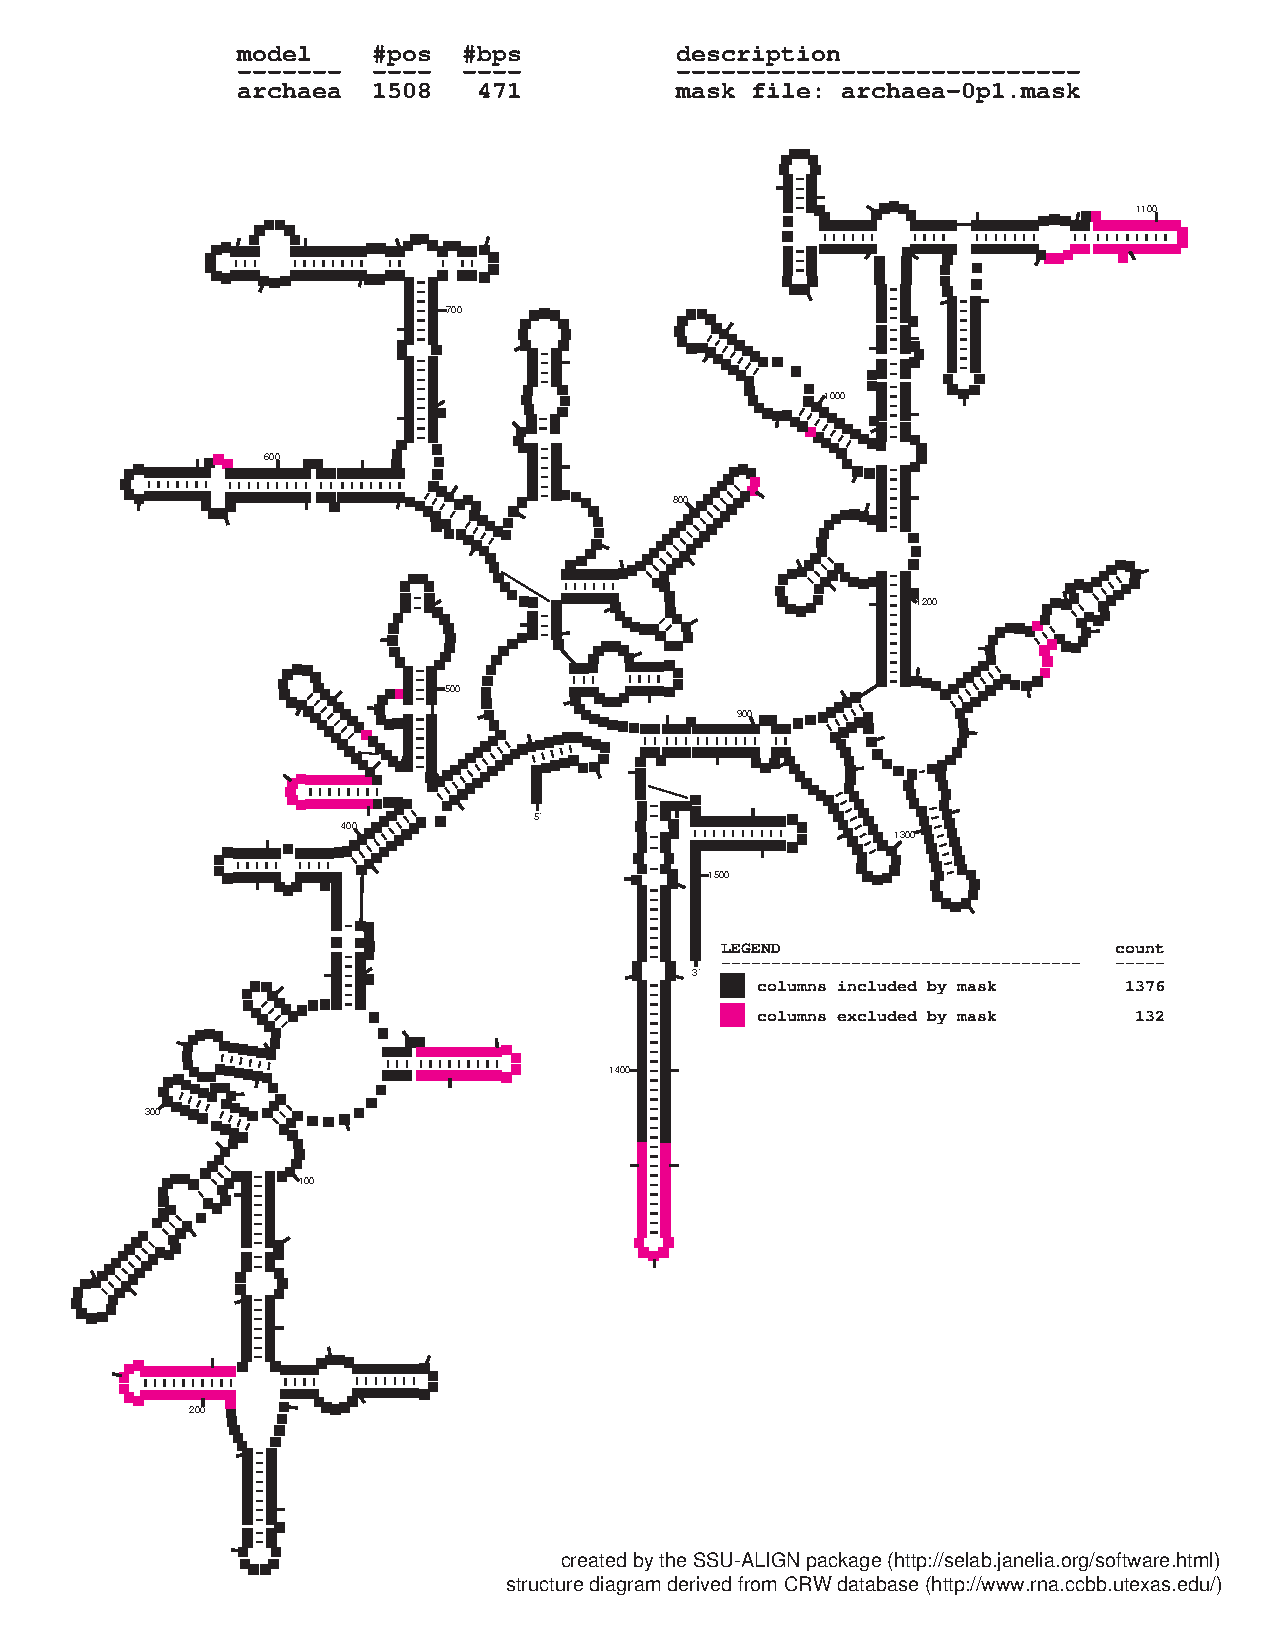
\includegraphics[width=4.2in]{Figures/archaea-0p1-mask}
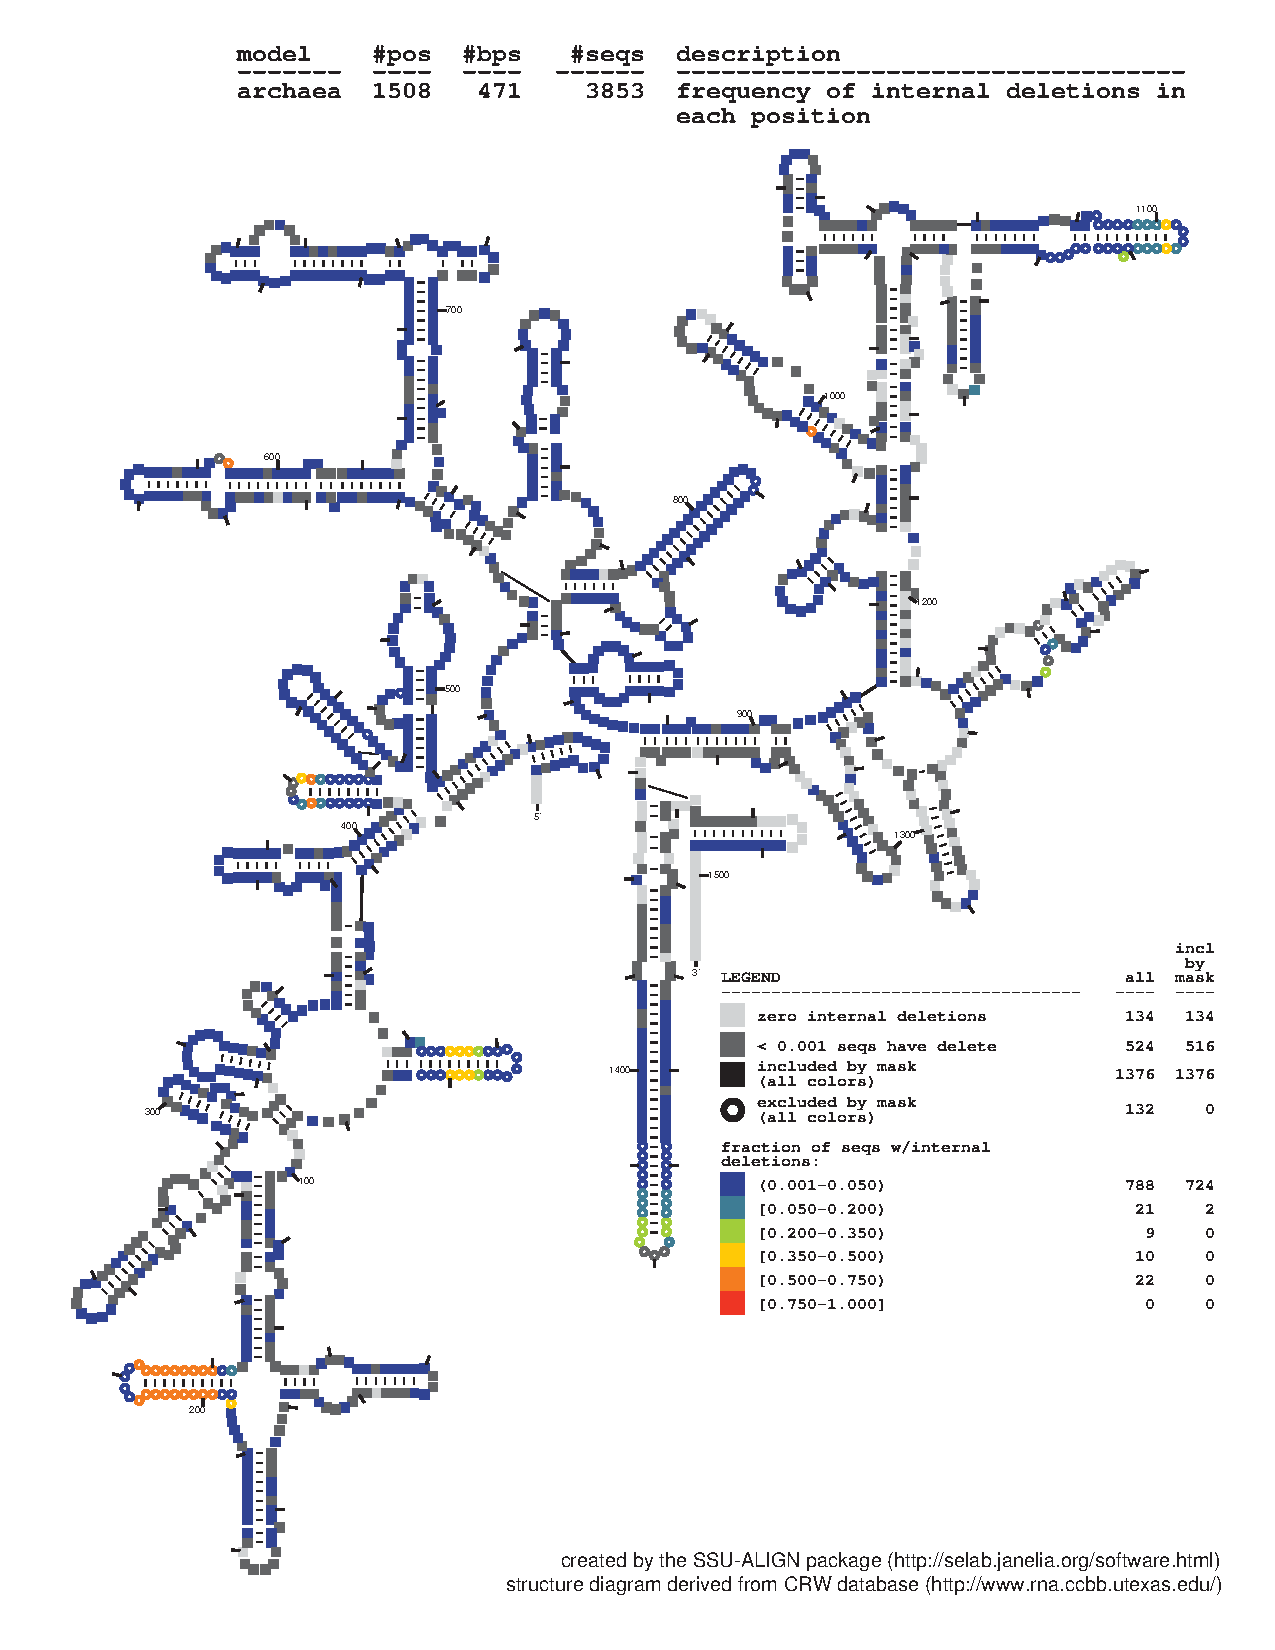
\includegraphics[width=4.2in]{Figures/archaea-ggsilR-dint-wmask}
  \end{center}
\caption{\textbf{Two diagrams of the default archaeal mask.} Left: pink positions are excluded,
  black positions are included. Right: Open circles are excluded,
  filled squares are included. Positions are colored based on
  frequency of deletions (gaps) in the filtered alignment of archaea
  from \textsc{greengenes} and \textsc{silva} \emph{Ref} (see text) as
  indicated in the legend.}
\label{fig:mask-arc}
\end{sidewaysfigure}

\begin{sidewaysfigure}
  \begin{center}
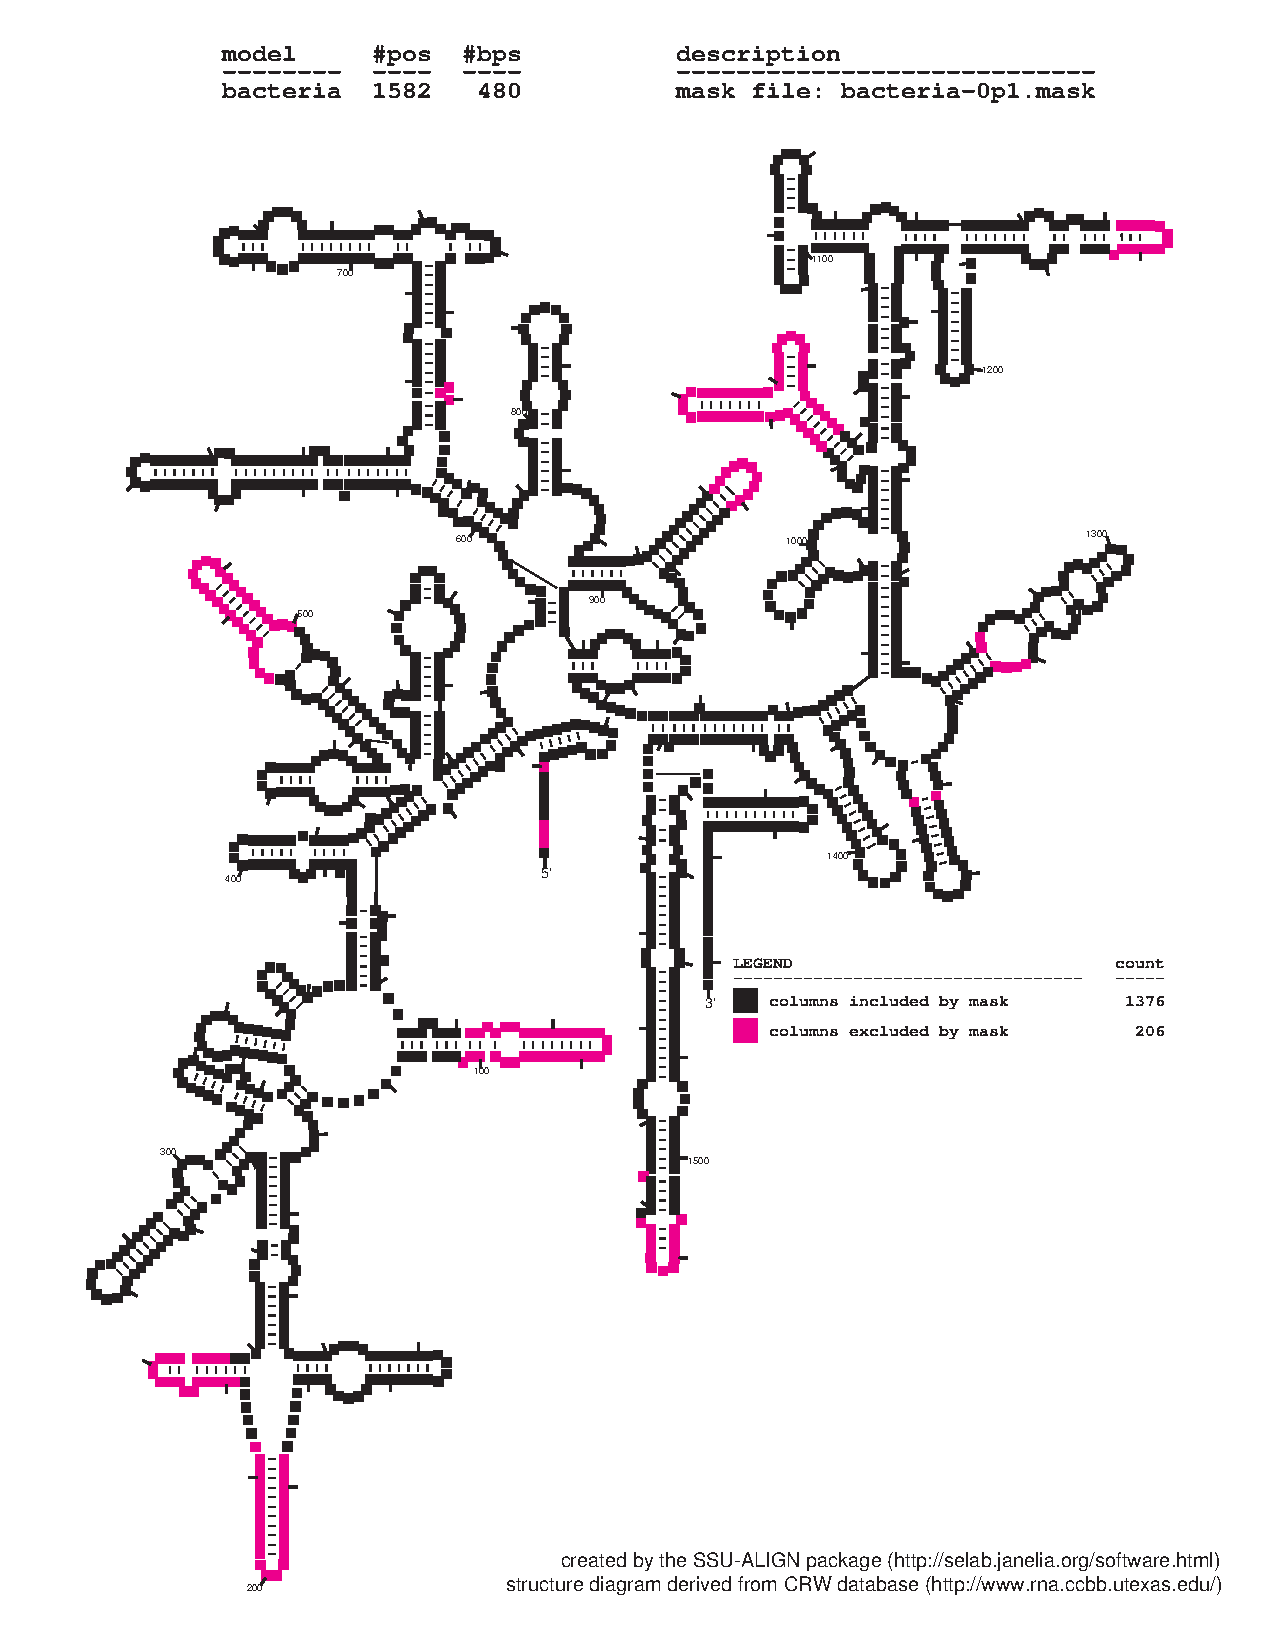
\includegraphics[width=4.2in]{Figures/bacteria-0p1-mask}
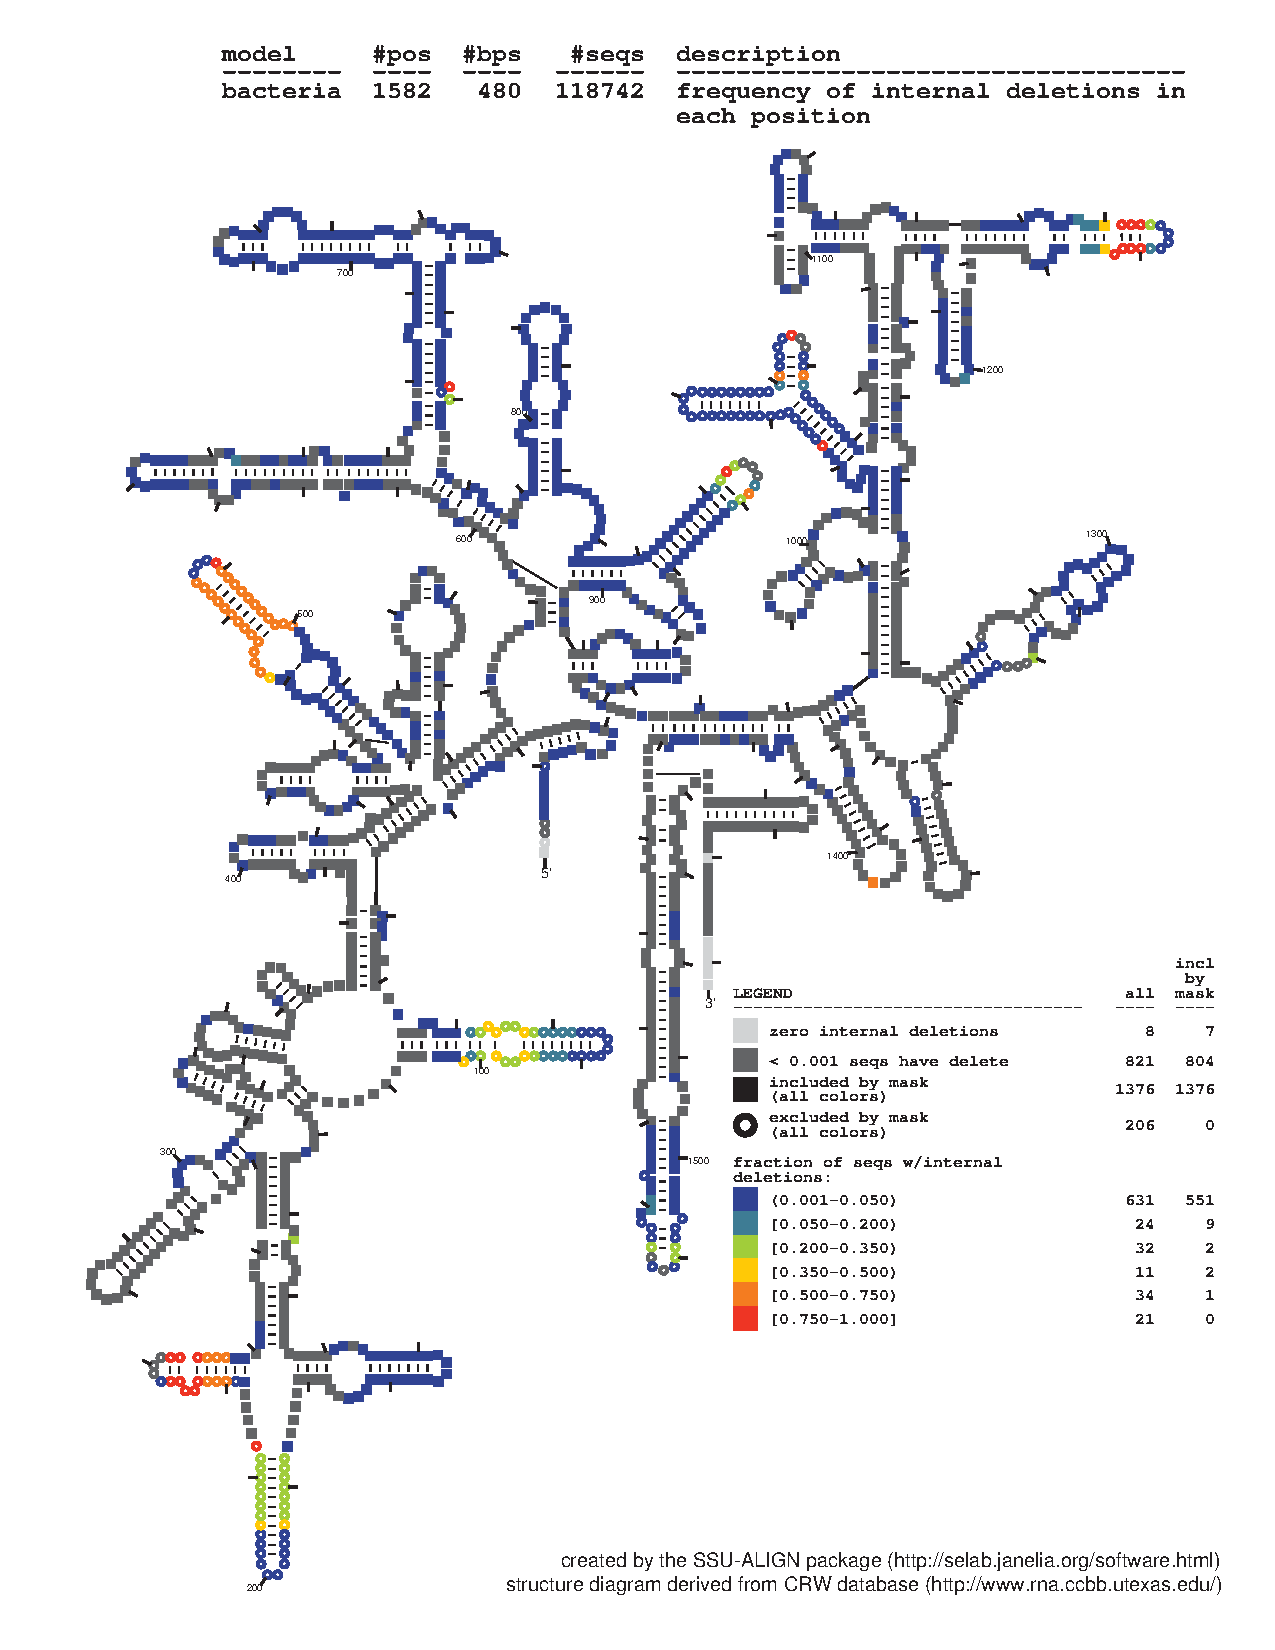
\includegraphics[width=4.2in]{Figures/bacteria-ggsilR-dint-wmask}
  \end{center}
\caption{\textbf{Two diagrams of the default bacterial mask.} Left: pink positions are excluded,
  black positions are included. Right: Open circles are excluded,
  filled squares are included. Positions are colored based on
  frequency of deletions (gaps) in the filtered alignment of bacteria
  from \textsc{greengenes} and \textsc{silva} \emph{Ref} (see text) as
  indicated in the legend.}
\label{fig:mask-bac}
\end{sidewaysfigure}

\begin{sidewaysfigure}
  \begin{center}
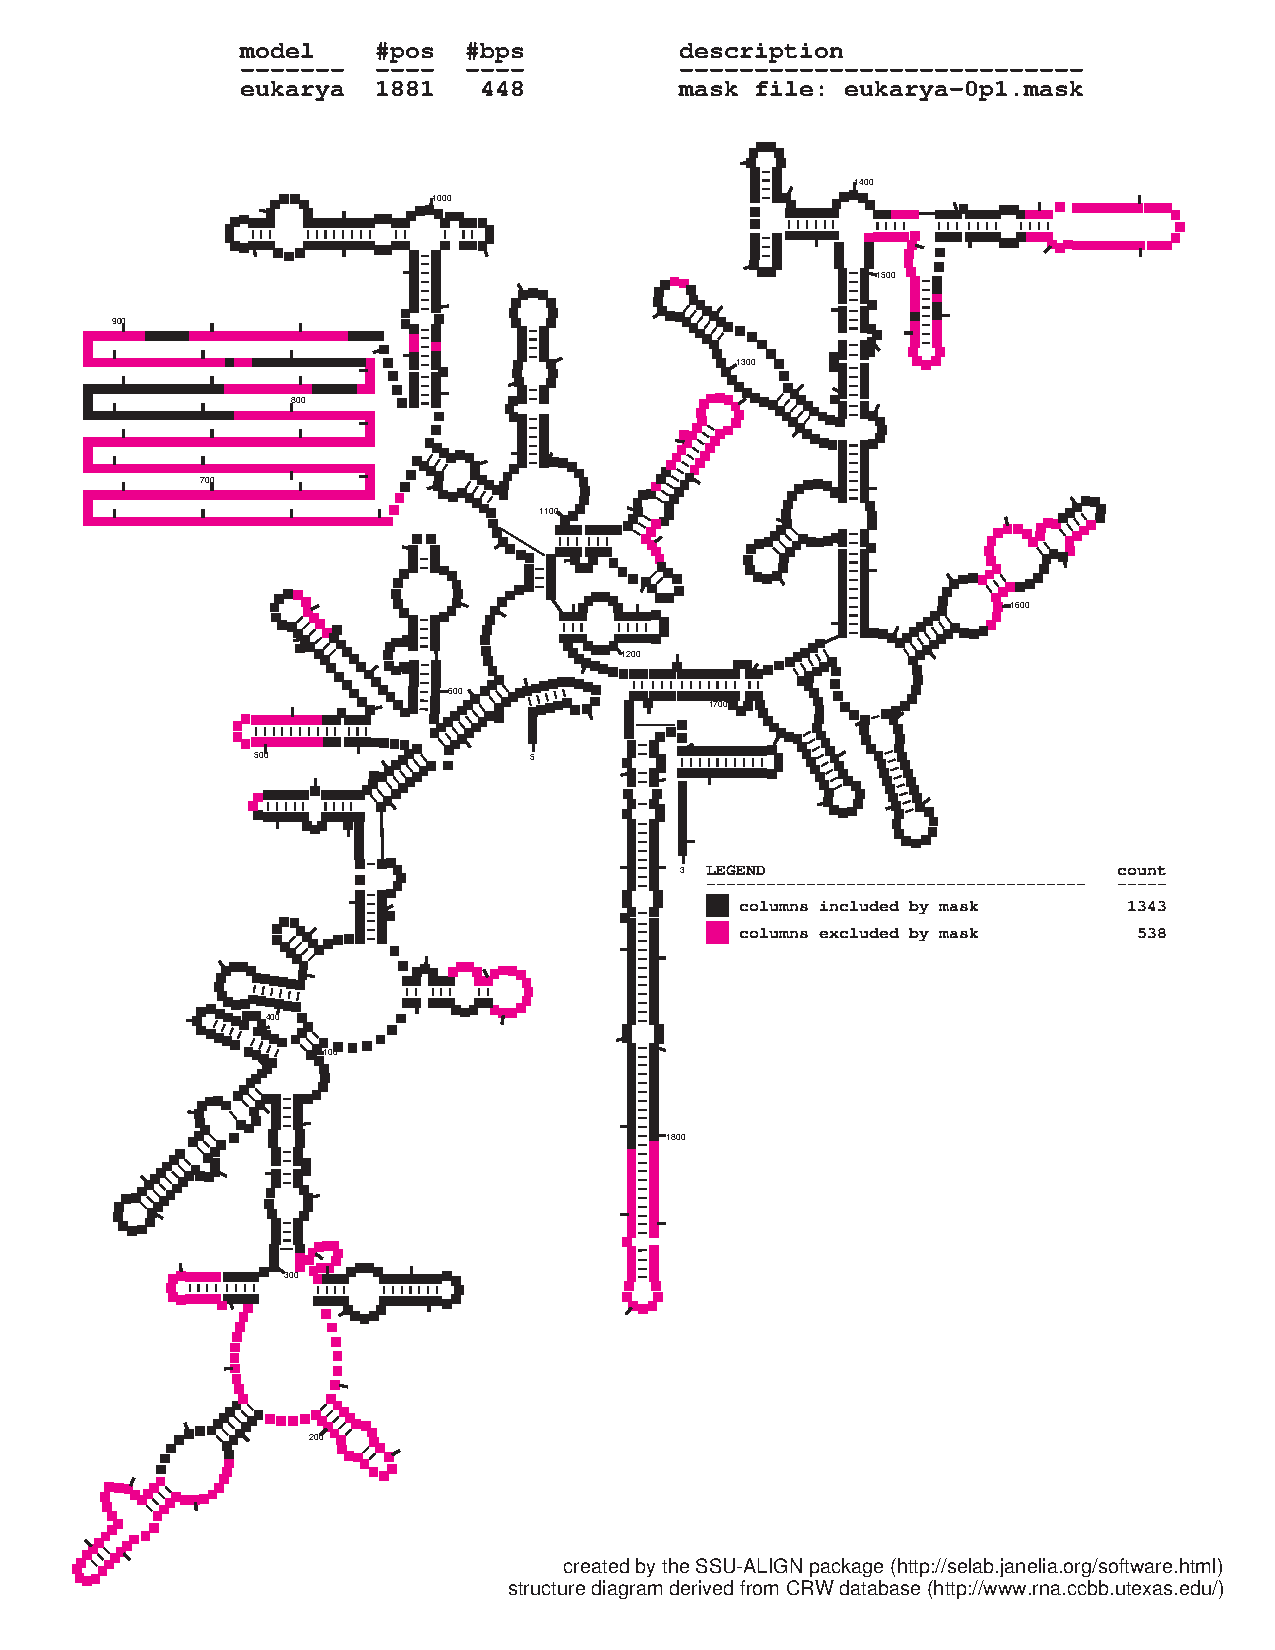
\includegraphics[width=4.2in]{Figures/eukarya-0p1-mask}
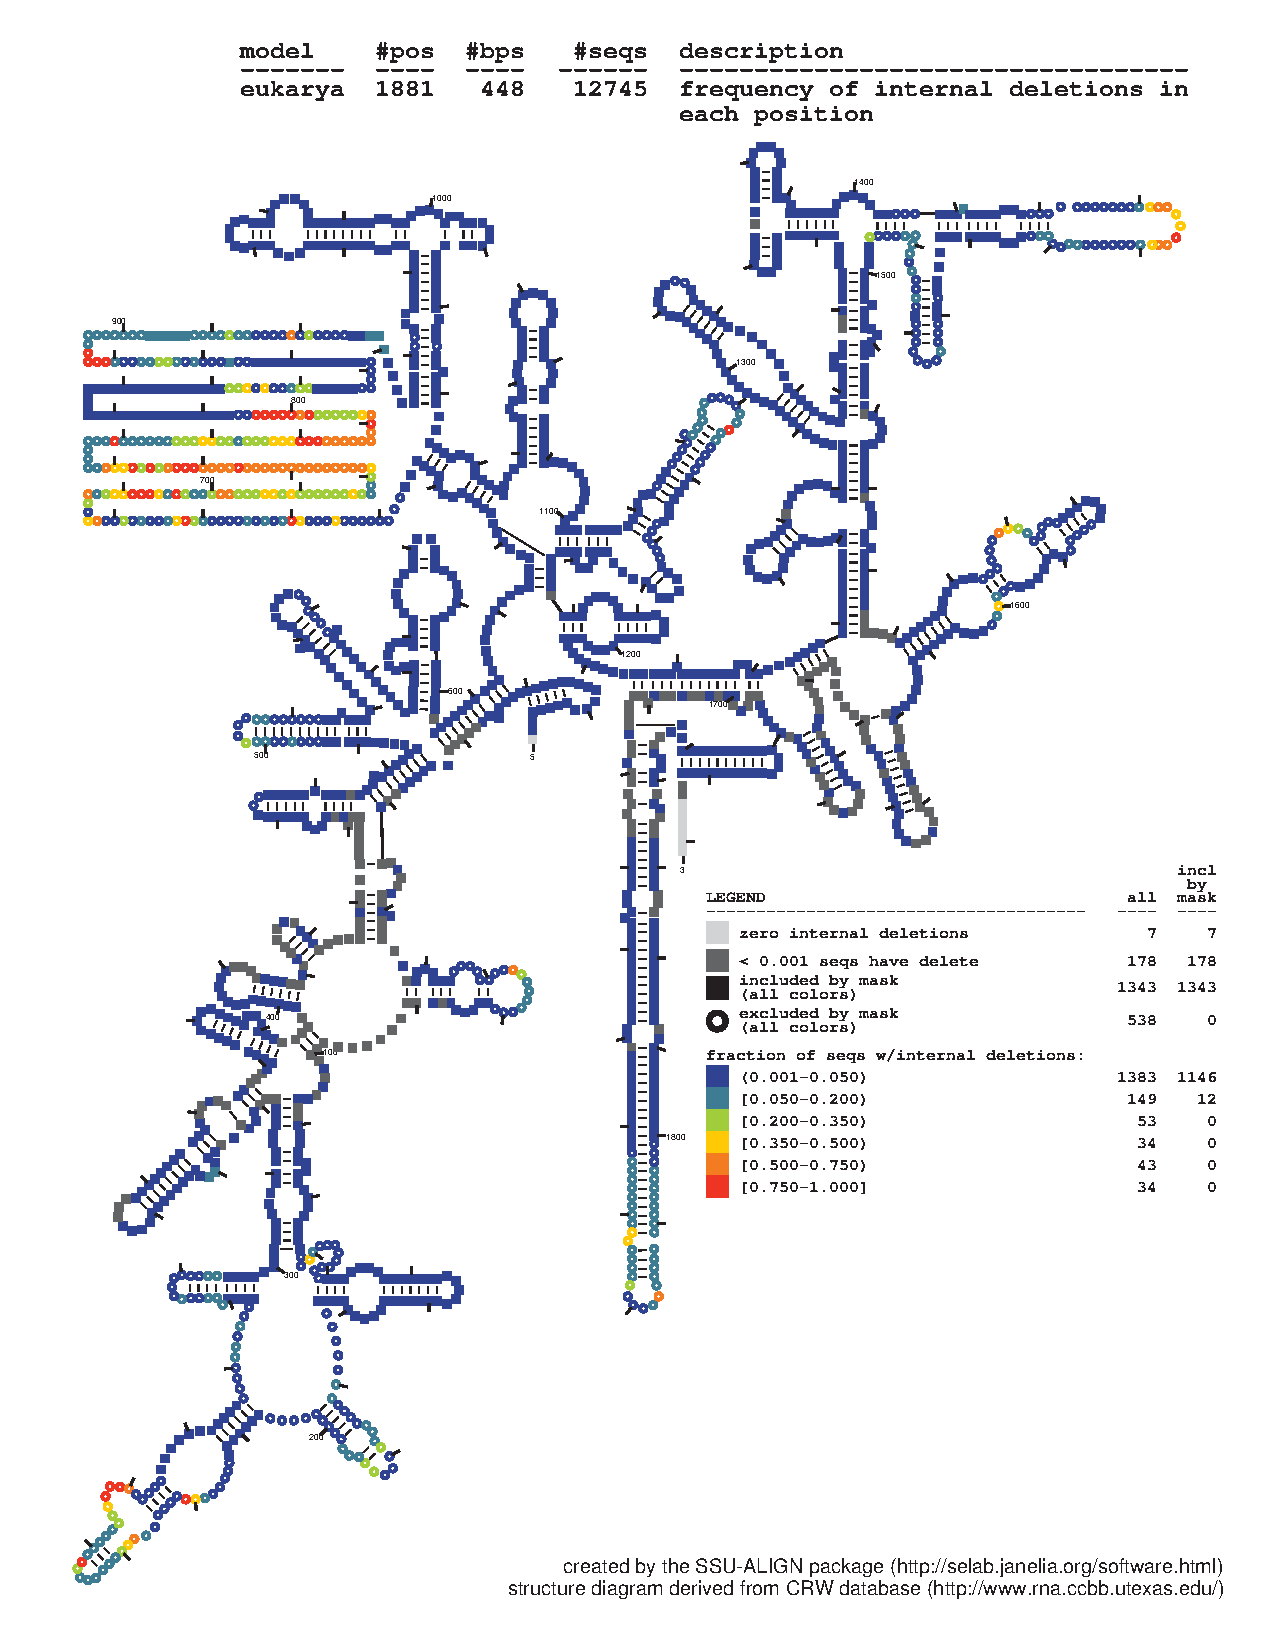
\includegraphics[width=4.2in]{Figures/eukarya-ggsilR-dint-wmask}
  \end{center}
\caption{\textbf{Two diagrams of the default eukaryotic mask.} Left: pink positions are excluded,
  black positions are included. Right: Open circles are excluded,
  filled squares are included. Positions are colored based on
  frequency of deletions (gaps) in the filtered alignment of eukarya
  from \textsc{greengenes} and \textsc{silva} \emph{Ref} (see text) as
  indicated in the legend.}
\label{fig:mask-euk}
\end{sidewaysfigure}

\newpage
\section{Description of output files}
\label{sec:output}

This section describes the content of the different output file
formats created by the various programs in the \textsc{ssu-align}
package. For demonstration, the descriptions below refer to the
specific files created during the tutorial in
section~\ref{sec:tutorial}, in the directory \prog{myseqs/}. 
Specifically, we'll go over the files created by the following four
commands from the tutorial:

\user{ssu-align seed-15.fa myseqs}

\user{ssu-mask myseqs} 

\user{ssu-draw myseqs}

\subsection{ssu-align output files}

As shown in the tutorial, when executed with the command above, \prog{ssu-align} 
prints information about the output files it creates to the screen:

\begin{sreoutput}
# Stage 1: Determining SSU start/end positions and best-matching models...
#
# output file name         description                                
# -----------------------  -------------------------------------------
  myseqs.tab               locations/scores of hits defined by HMM(s)
  myseqs.archaea.hitlist   list of sequences to align with archaea CM
  myseqs.archaea.fa              5 sequences to align with archaea CM
  myseqs.bacteria.hitlist  list of sequences to align with bacteria CM
  myseqs.bacteria.fa             5 sequences to align with bacteria CM
  myseqs.eukarya.hitlist   list of sequences to align with eukarya CM
  myseqs.eukarya.fa              5 sequences to align with eukarya CM
#
# Stage 2: Aligning each sequence to its best-matching model...
#
# output file name         description
# -----------------------  ---------------------------------------
  myseqs.archaea.stk       archaea alignment
  myseqs.archaea.cmalign   archaea cmalign output
  myseqs.archaea.ifile     archaea insert info
  myseqs.bacteria.stk      bacteria alignment
  myseqs.bacteria.cmalign  bacteria cmalign output
  myseqs.bacteria.ifile    bacteria insert info
  myseqs.eukarya.stk       eukarya alignment
  myseqs.eukarya.cmalign   eukarya cmalign output
  myseqs.eukarya.ifile     eukarya insert info
  myseqs.scores            list of CM/HMM scores for each sequence
\end{sreoutput}

I'll walk through the format of these output files:

\subsubsection{.tab suffixed files}

The \prog{.tab} files are created by \textsc{infernal}'s
\prog{cmsearch} program which is called internally by
\prog{ssu-align}. \prog{cmsearch} builds profile HMMs for each model
in the input CM file and scans each input sequence for high scoring
alignments to the HMM\@. The \prog{.tab} file lists the locations and
scores of each of these alignments. Let's look at the header of the 
\prog{seed-15.tab} file created here:

\begin{sreoutput}
# command:    ssu-cmsearch --hmm-cW 1.5 --no-null3 --noalign -T -1 --tab myseqs/myseqs.tab --viterbi 
/usr/local/share/ssu-align-0.1/ssu-align-0p1.cm seed-15.fa
# date:       Tue May 18 05:48:34 2010
# num seqs:   15
# dbsize(Mb): 0.040518
#
# Pre-search info for CM 1: archaea
#
# rnd  mod  alg  cfg   beta  bit sc cut
# ---  ---  ---  ---  -----  ----------
#   1  hmm  vit  loc      -       -1.00
#
\end{sreoutput}

The first four lines list the \prog{cmsearch} command executed from
within \prog{ssu-align}, the date it was executed, the number of
sequences in the sequence file being searched, and the number of
millions of nucleotides (Mb) searched in that sequence file (double the
actual size of the sequences because both strands are searched).

Next, the pre-search information describing how the search will be
conducted is printed for the first model in the CM file: \prog{archaea}. 
The \prog{rnd}, \prog{mod}, \prog{alg} and \prog{cfg} columns report
that the first and only round of searching will be conducted with a
profile \prog{hmm} using the \prog{vit}erbi algorithm for scoring
\prog{loc}al alignments to the model. The \prog{beta}
column is irrelevant when searching with an HMM\@. The \prog{bit sc cut}
column shows the minimum score threshold, alignments scoring above
\prog{-1.00} bits will be reported.

After the pre-search information comes four lines of column headings
followed by data lines reporting high scoring local alignments. One
line is printed per alignment, or \emph{hit} (it is possible to see
more than one hit per sequence). Remember these are scores against the
archaea model.

\begin{sreoutputtiny}
# CM: archaea
#                                                                      target coord   query coord                         
#                                                            ----------------------  ------------                         
# model name  target name                                         start        stop  start   stop    bit sc   E-value  GC%
# ----------  ---------------------------------------------  ----------  ----------  -----  -----  --------  --------  ---
  archaea     00052::Halobacterium_sp.::AE005128                      1        1473      1   1508   2080.08         -   58
  archaea     00052::Halobacterium_sp.::AE005128                   1229        1217      1   1508      1.41         -   54
  archaea     00013::Methanobacterium_formicicum::M36508              1        1476      1   1508   2108.16         -   56
  archaea     00013::Methanobacterium_formicicum::M36508           1227         984      1   1508      1.80         -   59
  archaea     00004::Nanoarchaeum_equitans::AJ318041                  1         865      1   1508   1112.07         -   67
  archaea     00004::Nanoarchaeum_equitans::AJ318041                619         570      1   1508      1.00         -   64
  archaea     00121::Thermococcus_celer::M21529                     202        1687      1   1508   2223.71         -   66
  archaea     00121::Thermococcus_celer::M21529                    1237        1188      1   1508      1.00         -   62
  archaea     00115::Pyrococcus_furiosus::U20163|g643670            260         309      1   1508      1.00         -   62
  archaea     00115::Pyrococcus_furiosus::U20163|g643670            922           1      1   1508   1354.25         -   66
  archaea     00035::Bacteroides_fragilis::M61006|g143965            60        1533      1   1508    576.22         -   51
  archaea     01106::Bacillus_subtilis::K00637                       55        1548      1   1508    768.61         -   55
  archaea     01106::Bacillus_subtilis::K00637                      684         672      1   1508     -0.63         -   46
  archaea     00072::Chlamydia_trachomatis.::AE001345               123         853      1   1508    212.41         -   51
  archaea     01351::Mycoplasma_gallisepticum::M22441               110         120      1   1508      1.43         -   36
  archaea     01351::Mycoplasma_gallisepticum::M22441               872          69      1   1508     95.30         -   45
  archaea     00224::Rickettsia_prowazekii.::AJ235272               104        1590      1   1508    613.67         -   51
  archaea     00224::Rickettsia_prowazekii.::AJ235272               748         739      1   1508      0.79         -   40
  archaea     01223::Audouinella_hermannii.::AF026040              1079        1767      1   1508    222.16         -   54
  archaea     01223::Audouinella_hermannii.::AF026040               880         871      1   1508      0.79         -   40
  archaea     01240::Batrachospermum_gelatinosum.::AF026045        1077        1761      1   1508    219.14         -   54
  archaea     01240::Batrachospermum_gelatinosum.::AF026045         878         869      1   1508      0.79         -   40
  archaea     00220::Euplotes_aediculatus.::M14590                  710        1081      1   1508     96.64         -   48
  archaea     00220::Euplotes_aediculatus.::M14590                  508         499      1   1508      0.79         -   40
  archaea     00229::Oxytricha_granulifera.::AF164122               335         344      1   1508      0.79         -   40
  archaea     00229::Oxytricha_granulifera.::AF164122               138          31      1   1508     86.31         -   53
  archaea     01710::Oryza_sativa.::X00755                         1190        1883      1   1508    202.90         -   53
  archaea     01710::Oryza_sativa.::X00755                          989         980      1   1508      0.79         -   40
\end{sreoutputtiny}

Here's a brief description of each column:

\begin{wideitem}
\item[\emprog{model name}] the name of the model used for the search.

\item[\emprog{target name}] the name of the target sequence.

\item[\emprog{start (target coord)}] first sequence nucleotide in the alignment

\item[\emprog{end (target coord)}] final sequence nucleotide in the alignment
\end{wideitem}

Note that under \prog{target coord} some of the sequences' \prog{start} position is
greater than their \prog{stop} positions. This occurs if the program
has determined the sequence in the target sequence file is a reverse
complemented SSU sequence. 

The \prog{start} and \prog{stop} columns under \prog{query coord} are
uninformative for HMM searches like these.
(\prog{cmsearch} will print informative numbers in
these columns when the CM is used for a search.) With HMM searches the
\prog{begin} column will always be \prog{1} and the \prog{end} column
will always be the final position of the model.

\begin{wideitem}

\item[\emprog{bit sc}] the bit score of the HMM alignment of
  target sequence nucleotides \prog{begin} to \prog{end}.

\item[\emprog{E-value}] this will always read \prog{-}. It would
  include an E-value of the bit score if the model had been calibrated
  with \prog{cmcalibrate}. Currently, \prog{ssu-align} does not use
  calibrated models, mainly because they are most useful for
  identifying remotely homologous structural RNAs using models of
  much smaller RNAs, such as transfer RNA. See the \textsc{infernal} 
  user's guide \cite{Nawrocki09} for more information.

\item[\emprog{GC\%}] the percent of the nucleotides in the aligned
  sequence that are either \prog{G} or \prog{C}. This is largely
  irrelevant for SSU rRNA, but is sometimes useful when using
  \prog{cmsearch} with smaller models.
\end{wideitem}

\subsubsection{.hitlist suffixed files}

The \prog{.hitlist} files are simple files created for each model
that list the sequences that were best-matches to that model, and as a
result were aligned to that model in stage 2. If a model has zero
sequences for which it is the best-matching model, this file will not
be created for that model. The file contains no new information that is not in the
\prog{.tab} file and is only created as a convenience, because it is
cumbersome to determine which model gave the highest score to a
particular sequence in the \prog{.tab} file.  For model \emph{x}, the
\prog{hitlist} file contains four columns providing four pieces of
data for each sequence whose best-matching model was \emph{x}. For
example, take a look at the \prog{myseq.archaea.hitlist}
file:

\begin{sreoutput}
# List of 5 subsequences to align to CM: archaea
# Created by ssu-align.
#
# target name                                  start    stop     score
# ------------------------------------------  ------  ------  --------
  00052::Halobacterium_sp.::AE005128               1    1473   2080.08
  00013::Methanobacterium_formicicum::M36508       1    1476   2108.16
  00004::Nanoarchaeum_equitans::AJ318041           1     865   1112.07
  00121::Thermococcus_celer::M21529              202    1687   2223.71
  00115::Pyrococcus_furiosus::U20163|g643670     922       1   1354.25
\end{sreoutput}

The four columns correspond to those of the same name in the \prog{.tab}
suffixed files as explained above: the \prog{target name},
\prog{start} and \prog{stop} (which correspond to the target sequence
coordinates), and \prog{score}, which is the primary sequence HMM
score assigned to this subsequence by model \emph{x}: the scores of
all other hits from this and other other models are less than
this score.

\subsubsection{.fa suffixed files}
This is a FASTA-formatted sequence file containing the sequences
listed in the corresponding \prog{hitlist} file. For example, the
file \prog{myseqs/myseqs.archaea.fa} contains the five sequences
listed in \\
\prog{myseqs/myseqs.archaea.hitlist}. These sequences were
copied from the original sequence file \prog{seed-15.fa} that
was used as input to \prog{ssu-align}. Only the nucleotides from
positions \prog{start} to \prog{stop} as listed in the
\prog{hitlist} file were copied, so sometimes the sequences in the
\prog{.fa} file will be subsequences of those from the original
file.  \prog{ssu-align} uses the \prog{.fa} files it
creates as input to the \prog{cmalign} program, which it calls
internally to generate its structurally annotated alignments.

\subsubsection{.cmalign suffixed files}

The \prog{.cmalign} files are the standard output created by the
\textsc{infernal} program \prog{cmalign} which is called internally
during the alignment stage of \prog{ssu-align}. There is one such file
created for each model that was the best-matching model to at least
one sequence in \prog{ssu-align}'s search stage. Take a look at the
beginning of the file \prog{myseqs.archaea.cmalign}:

\begin{sreoutputwide}
# command: ssu-cmalign --cm-name archaea --mxsize 4096 --no-null3 --sub --ifile myseqs/myseqs.archaea.ifile 
-o myseqs/myseqs.archaea.stk /usr/local/share/ssu-align-0.1/ssu-align-0p1.cm myseqs/myseqs.archaea.fa
# date:    Tue May 18 05:48:47 2010
#
# cm name                    algorithm  config  sub  bands     tau
# -------------------------  ---------  ------  ---  -----  ------
# archaea                      opt acc  global  yes    hmm   1e-07
\end{sreoutputwide}

This section includes the command used to execute \prog{cmalign}, the
date of execution, and information on the alignment parameters used by
the program.

The \prog{cm name} column reports the name of the model used for
alignment. \prog{algorithm} gives the name of the algorithm, in this
case \prog{opt acc} stands for \emph{optimal accuracy} \cite{Holmes98}
(also known as maximum expected accuracy). This algorithm is similar
to the CYK algorithm described in \cite{Nawrocki09b}, but returns the
alignment that maximizes the sum of posterior probability labels on
aligned nucleotides instead of the maximally scoring alignment. In
practice, for SSU the CYK and optimally accurate alignment are very often
identical, and if not, they are nearly identical.  The next two
columns, \prog{config} and \prog{sub}, read \prog{global} and
\prog{yes} respectively, which tells us the program will first predict
the start and end points of the alignment to the model using an HMM
(the \prog{sub yes} part) and then align the region of the model that
spans from start to end \emph{globally} to the sequence (the
\prog{global} part). In this case, \emph{global} alignment means that
the program is forced to align the full model region from start to end
to the sequence (it is \emph{not} allowed to skip large parts of the
model without large score penalties as it would if \emph{local}
alignment was being performed). The \prog{bands} column tells us that
bands (constraints) from an HMM alignment will be used to accelerate
alignment to the CM. This is explained more in Chapter 8 of
\cite{Nawrocki09b}. The \prog{tau} column reports the probability loss
allowed when computing the HMM bands. In this case, \prog{1e-07}
probability mass is allowed outside each band.

The next section includes per-sequence information on the alignment
that was created:

\begin{sreoutputwide}
#                                                                  bit scores                            
#                                                               ------------------                       
#   seq idx  seq name                                      len     total    struct  avg prob      elapsed
# ---------  ------------------------------------------  -----  --------  --------  --------  -----------
          1  00052::Halobacterium_sp.::AE005128           1473   2335.05    290.70     1.000  00:00:01.00
          2  00013::Methanobacterium_formicicum::M36508   1476   2331.84    262.88     0.999  00:00:01.01
          3  00004::Nanoarchaeum_equitans::AJ318041        865   1294.71    170.40     0.999  00:00:00.46
          4  00121::Thermococcus_celer::M21529            1486   2430.39    249.92     0.998  00:00:01.02
          5  00115::Pyrococcus_furiosus::U20163|g643670    922   1496.81    138.96     0.997  00:00:00.51
\end{sreoutputwide}

We'll go through each of these columns:

\begin{wideitem}
\item[\emprog{seq idx}] the index of the sequence in the file.

\item[\emprog{seq name}] the name of the sequence.

\item[\emprog{len}] length of the sequence; the full sequence hit from 
  the search stage is aligned, no trimming of ends is permitted, as it was in the search
  stage with \prog{cmsearch}.

\item[\emprog{total}] the bit score of the CM alignment. For more
  information, see section 5 of the \sft{infernal} User's Guide \cite{Nawrocki09}.

\item[\emprog{struct}] the secondary structure score component of the
  \prog{total} bit score. These are the added bits that are due solely
  to the modeling of the consensus secondary structure of the
  molecule by the CM\@. 
  
\item[\emprog{avg prob}] the average posterior labeling, or confidence
  estimate, of the aligned nucleotides. The higher this value is the less
  ambiguous and more well-defined the alignment is. The highest this
  can possibly be is \prog{1.000}, which means very nearly 100\% of
  the probability mass of the alignment to the model is contained in
  the single, optimally accurate alignment that was reported by the
  program. In other words, the reported alignment receives a
  significantly higher score than any other alternative alignment. The
  program derives this value by evaluating the score of every possible
  alignment (consistent with the HMM bands) of the sequence to the
  model, and comparing the best, optimal score versus all of the
  rest. 
  %This is described in a bit more detail in section~\ref{section:chap9}.

\item[\emprog{elapsed}] the amount of actual time (wall time) it took
  the program to align this sequence. In general, less well-defined
  alignments with lower \prog{avg prob} will take longer than more
  well-defined ones. This is because the HMM bands are usually tighter
  and act as stricter constraints to the CM alignment when the
  alignment is well-defined. Tighter bands lead to quicker alignments
  because fewer possible alignments to the CM must be considered.
\end{wideitem}

\subsubsection{.stk suffixed files}
The \prog{.stk} suffixed files are Stockholm-formatted alignment
files. These are the alignments generated by \prog{cmalign}. The
statistics in the \prog{.cmalign} suffixed files correspond to these
alignments. One alignment is created for each model that was the
best-matching model to at least one sequence in \prog{ssu-align}'s
search stage. An explanation of Stockholm alignments can be found at
the beginning of the tutorial, on page~\pageref{sec:tutorial-stk}.

\subsubsection{.scores suffixed files}

The \prog{.scores} file are meant to be a useful summary file.
They contain various statistics from each of the other output files
for every sequence in the original input sequence file. 

Take a look at the file \prog{myseqs.scores}:

\begin{sreoutputtinywide}
#                                                                        best-matching model                  second-best model 
#                                                         -------------------------------------------------  -------------------
#     idx  sequence name                                  model name   beg   end    CM sc   struct   HMM sc  model name   HMM sc  HMMdiff
# -------  ---------------------------------------------  ----------  ----  ----  -------  -------  -------  ----------  -------  -------
        1  00052::Halobacterium_sp.::AE005128             archaea        1  1473  2335.05   290.70  2080.08  bacteria     471.45  1608.63
        2  00013::Methanobacterium_formicicum::M36508     archaea        1  1476  2331.84   262.88  2108.16  bacteria     693.10  1415.06
        3  00004::Nanoarchaeum_equitans::AJ318041         archaea        1   865  1294.71   170.40  1112.07  bacteria     255.78   856.29
        4  00121::Thermococcus_celer::M21529              archaea      202  1687  2430.39   249.92  2223.71  bacteria     632.38  1591.33
        5  00115::Pyrococcus_furiosus::U20163|g643670     archaea      922     1  1496.81   138.96  1354.25  bacteria     378.49   975.76
        6  00035::Bacteroides_fragilis::M61006|g143965    bacteria       5  1537  2136.76   382.95  1797.77  archaea      576.22  1221.55
        7  01106::Bacillus_subtilis::K00637               bacteria       1  1552  2465.43   289.74  2212.50  archaea      768.61  1443.89
        8  00072::Chlamydia_trachomatis.::AE001345        bacteria       1   879  1215.64   183.53  1030.27  archaea      212.41   817.86
        9  01351::Mycoplasma_gallisepticum::M22441        bacteria     881     5  1165.86   217.01   940.15  archaea       95.30   844.85
       10  00224::Rickettsia_prowazekii.::AJ235272        bacteria      93  1594  2278.46   281.43  2037.49  archaea      613.67  1423.82
       11  01223::Audouinella_hermannii.::AF026040        eukarya        1  1770  2682.07   221.33  2481.69  archaea      222.16  2259.53
       12  01240::Batrachospermum_gelatinosum.::AF026045  eukarya        1  1764  2665.16   217.20  2463.49  archaea      219.14  2244.35
       13  00220::Euplotes_aediculatus.::M14590           eukarya        1  1082  1213.07    78.14  1103.29  archaea       96.64  1006.65
       14  00229::Oxytricha_granulifera.::AF164122        eukarya      600     1   851.30    23.53   788.12  archaea       86.31   701.81
       15  01710::Oryza_sativa.::X00755                   eukarya       75  1886  2687.06   142.17  2570.56  archaea      202.90  2367.66
\end{sreoutputtinywide}

There are four rows containing column headings prefixed with
\prog{\#}. Then there are 15 data rows, one for each sequence in the
input sequence file \prog{seed-15.fa}. Data rows are
separated into 12 columns:

\begin{wideitem}
\item[\emprog{idx}] the index of the sequence in the file.

\item[\emprog{sequence name}] the name of the sequence.
\end{wideitem}

The next 6 columns all describe the \emph{best-matching} model for the
sequence. This is the model that assigned the highest primary
sequence-based local profile HMM alignment score to the sequence.  If
no model aligned the sequence with a score higher than the minimum
threshold of 50 bits then the sequence was skipped and not aligned,
and all these columns will read \prog{-}. There are no such sequences
in the \prog{seed-15.fa} file, but if there were, an additional
\prog{.nomatch} file would have been created, as described
below. (Note: the minimum bit score
threshold value can be changed to \prog{<x>} using the
\prog{ssu-align} command-line option \prog{-b <x>}, as explained in
the \prog{ssu-align} anual page at the end of this guide).

\begin{wideitem}
\item[\emprog{model name}] name of best-matching model.

\item[\emprog{beg}] first nucleotide in the maximal
  scoring local HMM alignment to the best-matching model.

\item[\emprog{end}] final nucleotide in the maximal
  scoring local HMM alignment to the best-matching model.

\item[\emprog{CM sc}] the CM bit score for the best-matching model
  assigned to the sequence from positions \prog{beg} to \prog{end}.

\item[\emprog{struct}] the number of extra bits included in the
  CM bit score that are dervied from the secondary structure component
  of the model.

\item[\emprog{HMM sc}] the HMM bit score for the local alignment of
  the best-matching model to the sequence from positions \prog{beg} to
  \prog{end}.
\end{wideitem}

For more information on bit scores, see section 5 of the \sft{infernal}
User's Guide \cite{Nawrocki09}. 

The next 2 columns describe the \prog{second-best model}. This is the
model that assigned the second-highest primary sequence-based local 
profile HMM alignment score to the sequence. If only one models score
exceeded the minimum of 50 bits then these columns will each read
``\prog{-}''.

\begin{wideitem}
\item[\emprog{model name}] name of second-best-matching model.

\item[\emprog{HMM sc}] the HMM bit score for the local alignment of
  the second-best-matching model to the sequence. This alignment was
  not necessarily from \prog{beg} to \prog{end} (those were the
  coordinates of the alignment to the best-matching model). The
  sequence coordinates of the second-best model's alignment can be
  found in the file \prog{myseqs.tab}.
\end{wideitem}

The final column, \prog{HMMdiff}, reports the score difference between
the best-matching model HMM alignment and the second-best matching
model HMM alignment. This is included because it is an indication of
how clearly ``homologous'' the sequence is to the best-matching model
rather than to the second-best-matching model. The higher this score
difference is the more obvious it is that the sequence falls within
the sequence diversity represented by the best-matching model.
Sequences that are phylogenetically novel and do not obviously match
any single model much better than any other one should have relatively
small score differences in this column.

\subsubsection{.nomatch suffixed files}

A \prog{.nomatch} file simply lists the sequences in the input
sequence file that do not match to any model, one sequence name per
line. For a sequence to match to a model it must score above the
minimum profile HMM bit score threshold to at least one model. By
default, this threshold is 50 bits, but it can be changed to
\prog{<x>} bits with the \prog{-b <x>} option to \prog{ssu-align}. All
15 sequences in the tutorial file \prog{seed-15.fa} score above this
threshold to at least one model, so no \prog{.nomatch} file is
created. 

\subsection{.sum suffixed files}

The \prog{.sum} files include the text reported to the screen
(standard output) by \prog{ssu-align}. These files serve as a
reference to remind the user how \prog{ssu-align} was run
(parameters, input file names, etc.). All six programs in the
\textsc{ssu-align} package generate specifically named \prog{.sum}
suffixed files. For example, \prog{ssu-mask} generates a file ending
with the suffix \prog{.ssu-mask.sum}.

As a special case, when \prog{ssu-prep} is used to create parallel
jobs of \prog{ssu-align}, a \prog{ssu-prep.sum} file is created. Then,
when the \prog{ssu-prep}-generated shell script that executes the
parallel alignment jobs is run, a \prog{ssu-align.sum} file will be created.
This \prog{ssu-align.sum} file will contain the 
\prog{ssu-align.sum} files from all parallel alignment jobs
concatenated together, followed by a section describing the merge
performed automatically by the final job and alignment
statistics summarizing all parallel jobs.

\prog{ssu-align.sum} files include more information than the other
program's \prog{.sum} files. Specifically, they include two sections
labelled \prog{Summary statistics} and \prog{Speed statistics} which
summarizes the number of sequences in the input target sequence file
that match each model, and how fast the program completed the search
and alignment stages, respectively. Below is a short description of
each of the fields in the \prog{Summary statistics} section of the
\prog{myseqs.ssu-align.sum} file we just created:

\begin{sreoutput}
# Summary statistics:
#
# model or       number  fraction        average   average               
# category      of seqs  of total         length  coverage    nucleotides
# ------------  -------  --------  -------------  --------  -------------
  *input*            15    1.0000        1350.60    1.0000          20259
#
  archaea             5    0.3333        1244.40    0.9546           6222
  bacteria            5    0.3333        1268.60    0.9793           6343
  eukarya             5    0.3333        1405.60    0.9675           7028
#
  *all-models*       15    1.0000        1306.20    0.9671          19593
  *no-models*         0    0.0000              -         -              0
\end{sreoutput}

\begin{wideitem}
\item[\emprog{model or category}] the name of the model or category
  the row pertains to. Categories include \prog{*input*}, the set of 
  all full length target sequence file used as input; \prog{*all-models*},
  the set of sequences that match any model; and \prog{*no-models*}, the set of
  sequences that do not match any model above threshold. 

\item[\emprog{number of seqs}] number of seqs that belong in a
  category, or were best-matches to a model.

\item[\emprog{fraction of total}] the number of sequences in this
  model/category divided by the total number of sequences listed in the
  \prog{*input*} category.

\item[\emprog{average length}] the average sequence length of the
  model/category. For models, this is the average length of the
  subsequences that survive the search stage, which are not
  necessarily the full length sequences in the input sequence file.

\item[\emprog{average coverage}] length of suriviving sequences
  divided by the full length of those sequences in the input sequence
  file. 

\item[\emprog{nucleotides}] summed length of suriviving sequences in
  model/category. This is equal to the product of the values in
  \prog{number of seqs} and \prog{average length} columns.
\end{wideitem}

Now, take a look at the \prog{Speed statistics} section. Each field in
this table is described below:

\begin{sreoutput}
# Speed statistics:
#
# stage      num seqs  seq/sec  seq/sec/model    nucleotides    nt/sec
# ---------  --------  -------  -------------  -------------  --------
  search           15    1.159          0.386          20259    1565.5
  alignment        15    0.972          0.972          19593    1270.0
\end{sreoutput}

\begin{wideitem}
\item[\emprog{stage}] the stage of the program this row pertains to,
  either \prog{search} or \prog{alignment}.

\item[\emprog{num seqs}] the number of sequences processed by this stage.

\item[\emprog{seq/sec}] the number of sequences processed by this
  stage per second.

\item[\emprog{seq/sec/model}] the number of sequences processed by this
  stage per second per model. This is the value in the \prog{seq/sec}
  column divided by the number of models used to search for or align
  the sequences. Remember that in the \prog{search} stage, all 3
  models are used by default, whereas only 1 model is used in the
  \prog{alignment} stage (figure~\ref{fig:strategy}).

\item[\emprog{nucleotides}] summed length of all sequences processed
  by this stage.

\item[\emprog{nt/sec}] number of nucleotides processed by this stage
  per second.
\end{wideitem}

\subsection{.log suffixed files}

The \prog{.log} files include information on all of the system
commands run by \prog{ssu-align}. As with \prog{.sum} suffixed files,
program specific \prog{.log} suffixed files are created by each of the
six \textsc{ssu-align} programs. For example, \prog{ssu-mask}
generates a log file ending with the suffix \prog{.ssu-mask.log}.


As a special case, when \prog{ssu-prep} is used to create parallel
jobs of \prog{ssu-align}, a \prog{ssu-prep.log} file is created. Then,
when the \prog{ssu-prep}-generated shell script that executes the
parallel alignment jobs is run, a \prog{ssu-align.log} file will be created.
This \prog{ssu-align.log} file will contain the 
\prog{ssu-align.log} files from all parallel alignment jobs
concatenated together.

The \prog{.log} files list all of the commands that were executed by
the program along with their STDERR and sometimes their STDOUT output
(for example, the \prog{cmsearch} and \prog{cmalign} commands), as
well as the ``globals hash'', a set of variables defined in the
\textsc{ssu-align} PERL module \prog{ssu.pm} which is installed in the
\$SSUALIGNDIR. The \prog{.log} files should mainly be useful to expert 
users or developers who are trying to figure out why a specific run of a
program failed, or how to reproduce a specific step executed by the
program (e.g. the \prog{cmsearch} step of \prog{ssu-align}).

\subsection{ssu-mask output files}

The \prog{ssu-mask} example from the tutorial is executed with:

\user{ssu-mask myseqs} 

This command generates three output files per-domain, each of which is
briefly explained below. These files are also discussed in the
Tutorial section. 

\subsubsection{.mask suffixed files}
Mask files are simple one-line text files that correspond to a
specific domain model/alignment file and include only \prog{0} and
\prog{1} characters. Each character corresponds to a consensus column
of the model/alignment. For example, the
\prog{myseqs.archaea.mask} file contains 1508 characters, one per
consensus column of the default \textsc{ssu-align} archaeal model
described in section~\ref{sec:models}. A \prog{0} at position \emph{x}
indicates that consensus position \emph{x} is excluded from the mask
and will be removed from the alignment when the mask is applied. A
\prog{1} at position \emph{x} indicates that it is included by the
mask and will be kept when the mask is applied. A consensus position
of an alignment is one where the \prog{\#=GC RF} annotation is a
nongap (see section~\ref{sec:background} for more detail).

\subsubsection{.mask.pdf and .mask.ps suffixed files}
These are structure diagram files that display a mask on the consensus
secondary structure of a domain. Pink positions are excluded by the
mask. Black positions are included by the mask. Either \prog{.pdf} or
postscript \prog{.ps} files will be created, but not both. If you have
the program \prog{ps2pdf} in your path, \prog{.pdf} files will be
created, otherwise postscript will be. One difference between
these filetypes is their sizes, the PDF files created by
\prog{ssu-mask} are only about 10\% the size of the postscript files.

\subsubsection{.mask.stk suffixed files}
The \prog{.mask.stk} files are Stockholm-formatted alignment files
that include a subset of the columns of the alignments created by
\prog{ssu-align}. The consensus columns excluded by the mask have been
removed. Additionally, all insert columns have been removed. An insert
column is one which is a gap in the reference (\prog{\#=GC RF})
annotation of the alignment. For more information on inserts, see
section~\ref{sec:background}.

\subsubsection{.list suffixed files}
\prog{.list} suffixed files are only generated if \prog{ssu-mask} is
executed using the \prog{--list} option. A list file is generated for
a specific alignment file, and it simply lists the name of each
sequence in the alignment, one per line.

\subsubsection{.afa suffixed files}
\prog{.afa} suffixed files are FASTA-formatted alignment files that
are created by \prog{ssu-mask} only if the \prog{--stk2afa} option is
used. These files differ from unaligned FASTA files in that each
sequence may contain gaps, and all sequences are guaranteed to be
the same length. \prog{.afa} files created by \prog{ssu-mask}
contain two types of gap characters. A \prog{-} character
is a gap in a consensus column of an alignment. A \prog{.} character
is a gap in an insert column of an alignment. See
section~\ref{sec:background} for more information on the distinction
between consensus and insert columns. Note that \prog{.afa} alignment
files do not include structure information that is included in
Stockholm alignment files.

\subsection{ssu-draw output files}

The \prog{ssu-draw} example from the tutorial is executed with:

\user{ssu-draw myseqs} 

This command generates two output files per-domain, each of which is 
briefly explained below. 

\subsubsection{.pdf or .ps suffixed files}
These are structure diagram files that display either alignment
summary statistics (such as information content or frequency of gaps)
or individual aligned sequences on the consensus secondary structure
for a domain. They may be multiple pages. A brief description is
included at the top of each page. Along with each of these files, a
corresponding \prog{.drawtab} file is generated, as described below.
Either \prog{.pdf} or postscript \prog{.ps} files will
be created, but not both. If you have the program \prog{ps2pdf} in
your path, \prog{.pdf} files will be created, otherwise postscript
will be. One difference between
these filetypes is their sizes, the PDF files created by
\prog{ssu-draw} are only about 10\% the size of the postscript files.

\subsubsection{.drawtab suffixed files}
\prog{.drawtab} suffixed files are tab-delimited text files meant to
be easily parseable that contain the information displayed in a
corresponding \prog{.pdf} or \prog{.ps} structure diagram file. 
In these files, lines beginning with \prog{\#} are comment
lines. Comments at the beginning of \prog{.drawtab} files explain the
meaning of each of the tab-delimited fields in the non-comment lines. 


\newpage
\include{manpages}

\newpage
\section*{Index of frequently asked questions}
\listoffaqs

\newpage
\bibliography{master,lab,epn_thesis}
\end{document}
